\documentclass[11pt,a4paper]{article}
\usepackage[margin=2.25cm]{geometry}
\usepackage[T1]{fontenc}
\usepackage[utf8]{inputenc}
\usepackage[french]{babel}
\usepackage{booktabs}
\usepackage{graphicx}
\usepackage{hyperref}
\usepackage{amsmath}
\usepackage{float}
\usepackage{longtable}
\usepackage{placeins}
\usepackage{tabularx}
\usepackage{pdflscape}

\title{Etude de sensibilite du modele sans banque\\Rapport final provisoire et autonome}
\author{modele-27-04-WIP / studies/sensitivity}
\date{Mai 2026 -- version integrant les campagnes adaptatives (1\,479 runs)}

\begin{document}
\maketitle

\begin{abstract}
Ce rapport documente l'etude de sensibilite numerique du modele
\texttt{modele-27-04-WIP}. Le cadre principal est volontairement homogene :
\(\alpha_{\min}=\alpha_{\max}=1\). La volatilite brownienne
\(\sigma_\alpha=\texttt{alpha\_sigma\_brownien}\) varie en revanche comme un
parametre dynamique. Le taux d'amortissement est exclu. Les resultats montrent
que l'apparition d'un regime borne est principalement un phenomene de seuil :
\(k=\texttt{n\_candidats\_pool}\), \(\sigma_\alpha\), \(\theta\), \(\mu\),
les depreciations, la dotation initiale et \(\lambda=\texttt{lambda\_creation}\)
peuvent faire basculer le systeme entre croissance peu financee, regime dense,
et fragmentation numerique en micro-credits. L'objectif predictif est
partiellement atteint : sur les 193 observations disponibles, un modele simple
predit l'indicateur \texttt{bounded\_tail} avec une balanced accuracy de
0.84, et explique environ 0.58 de la variance de la densite financiere et
0.60 de la variance de \(\log(n_{\mathrm{alive}})\). Ces chiffres ne sont pas
un resultat final de machine learning ; ils quantifient surtout que les
parametres contiennent deja une information predictive forte.
\end{abstract}

\section{Perimetre et conventions}

Le modele simule des entites productives qui investissent, pretent, empruntent
et peuvent faire faillite par insolvabilite. Les grandeurs principales suivies
sont :
\begin{itemize}
  \item \(n_{\mathrm{alive}}\), nombre d'entites vivantes ;
  \item \(A\), actif total du systeme ;
  \item \(L\), nombre de prets actifs ;
  \item \(V\), volume financier des prets ;
  \item \(d_f = V/A\), densite financiere en volume (\texttt{densite\_fin\_mean}) ;
  \item \(\ell = L/n_{\mathrm{alive}}\), densite en nombre de contrats par entite ;
  \item \(r_f = \bar{f}/\lambda\), ratio faillites/creation (\texttt{failure\_lambda\_ratio}) ;
  \item \(G\), coefficient de Gini de l'actif entre entites ;
  \item le critere operationnel \(\mathcal{B}\) (\texttt{bounded\_tail}) : voir section~\ref{sec:protocole}.
\end{itemize}

\paragraph{Notation canonique.}
Le tableau suivant fixe la correspondance entre les symboles du rapport et
les noms de code.

\begin{center}
\small
\begin{tabular}{lll}
\toprule
Symbole & Code \texttt{snake\_case} & Signification \\
\midrule
\(k\) & \texttt{n\_candidats\_pool} & candidats evalues par emprunteur par pas \\
\(\lambda\) & \texttt{lambda\_creation} & taux de creation d'entites (reel) \\
\(\mu\) & \texttt{mu} & prime minimale de rendement a l'emprunt \\
\(\theta\) & \texttt{theta} & part du gain extraite a chaque pas \\
\(\delta\) & \texttt{taux\_depreciation\_endo} & taux de depreciation endogene \\
\(\sigma_\alpha\) & \texttt{alpha\_sigma\_brownien} & volatilite brownienne du rendement \\
\(f\) & \texttt{fraction\_taux\_emprunteur} & fraction du taux a charge de l'emprunteur \\
\(\phi\) & \texttt{fraction\_auto\_investissement} & part du gain reinvesti \\
\(\epsilon\) & \texttt{epsilon} & seuil de convergence numerique \\
\(d_f\) & \texttt{densite\_fin\_mean} & densite financiere en volume \(V/A\) \\
\(\ell\) & \texttt{loan\_density\_mean} & prets par entite vivante \(L/n_{\mathrm{alive}}\) \\
\(r_f\) & \texttt{failure\_lambda\_ratio} & ratio faillites/creation \(\bar{f}/\lambda\) \\
\(\mathcal{B}\) & \texttt{bounded\_tail} & critere de queue bornee (voir section~\ref{sec:protocole}) \\
\bottomrule
\end{tabular}
\end{center}

Le parametre \(\lambda=\texttt{lambda\_creation}\) est le taux du processus de
creation d'entites. Il est reel : il n'a pas a etre entier. Les premieres
grilles ont surtout utilise \(\lambda\in\{1,2,4\}\), mais les prochaines grilles
fines devront utiliser des valeurs intermediaires.

\section{Regime permanent : critere retenu}
\label{sec:critere-regime}

Le regime permanent ne se reduit pas a une chute forte de 25\,\% du nombre
d'entites. Une simulation utile peut avoir une chute faible, une stabilisation
tardive ou meme une decorrelation entre \(n_{\mathrm{alive}}\) et l'actif.

Le critere operationnel \(\mathcal{B}\) (\texttt{bounded\_tail}), calcule sur
la fenetre de queue $[t_{\mathrm{mesure}}, T]$ ou
$t_{\mathrm{mesure}} = \max(0.6\,T,\;t_{\mathrm{chute5}} + 100)$, est satisfait
si et seulement si les quatre conditions suivantes sont reunies
(voir \texttt{run\_simulation.py:detect\_regime\_diagnostics}) :
\[
  |\text{pente relative de }n_{\mathrm{alive}}| \le 0.20
  \quad\text{ET}\quad
  |\text{pente relative de }A| \le 0.20
\]
\[
  \text{IQR relatif de }n_{\mathrm{alive}} \le 0.70
  \quad\text{ET}\quad
  \text{IQR relatif de }A \le 0.80.
\]
La pente relative est le coefficient de la regression lineaire sur la queue,
divise par la valeur moyenne sur cette queue.
L'IQR relatif est l'ecart interquartile divise par la mediane.

Le critere \(\mathcal{B}\) n'est pas une preuve mathematique de stationnarite.
C'est un critere operationnel : il signale que, sur l'horizon observe, les
stocks ne continuent pas une derive de grande amplitude.

Le critere dual de stationnarite complete ajoute l'equilibre des flux :
$\mathcal{B} \wedge |r_f - 1| < 0.15$, ou $r_f = \bar{f}/\lambda$ est le
ratio moyen faillites/creation sur la fenetre de queue.

\section{Protocole experimental}
\label{sec:protocole}

\subsection*{Parametres du modele}

\begin{table}[H]
\centering
\small
\begin{tabularx}{\linewidth}{llXrr}
\toprule
Symbole & Code & Signification & Nominal $C_3$/$C_4$ & Plage testee \\
\midrule
$k$ & \texttt{n\_candidats\_pool} & candidats evalues par emprunteur par pas & 3 / 4 & 2--8 \\
$\lambda$ & \texttt{lambda\_creation} & taux de creation d'entites (reel) & 2.0 & 0.5--6.0 \\
$\mu$ & \texttt{mu} & prime minimale de rendement a l'emprunt & 0.05 & 0--0.15 \\
$\theta$ & \texttt{theta} & part du gain extraite par pas & 0.35 & 0.15--0.55 \\
$\delta$ & \texttt{taux\_depreciation\_endo} & taux de depreciation endogene & 0.05 & 0.01--0.15 \\
$\sigma_\alpha$ & \texttt{alpha\_sigma\_brownien} & volatilite brownienne du rendement & 0.0 & 0--0.10 \\
$f$ & \texttt{fraction\_taux\_emprunteur} & fraction du taux a charge emprunteur & 0.2 & 0.0--0.5 \\
$\phi$ & \texttt{fraction\_auto\_investissement} & part du gain reinvesti & 0.5 & 0.25--0.5 \\
$\epsilon$ & \texttt{epsilon} & seuil de convergence numerique & $10^{-3}$ & $10^{-6}$--$10^{-2}$ \\
\bottomrule
\end{tabularx}
\caption{Parametres varies dans l'etude. La valeur nominale est celle des
centres OAT. \texttt{taux\_amortissement} est fixe a 0 ; les parametres de
reliquefaction (\texttt{coefficient\_reliquefaction}, \texttt{seuil\_ratio\_liquide\_passif})
ont un effet nul mesure et sont exclus. Dans les campagnes
\(\theta\times\delta\), \(\delta_{\mathrm{endo}} = \delta_{\mathrm{exo}} = \delta_{\mathrm{liquide}}\)
(depreciation unifiee).}
\end{table}

\subsection*{Centres OAT}

L'analyse OAT (\emph{One-At-a-Time}) consiste a partir d'un vecteur de
parametres de reference (le \emph{centre}) et a faire varier un seul parametre
a la fois, tous les autres restes a leur valeur nominale. L'effet mesure est
le delta de metrique par rapport au resultat du centre.

Deux centres sont utilises, partageant le meme vecteur de parametres
sauf pour $k$ :

\begin{description}
  \item[$C_3$ (\texttt{subcritical\_k3})] :
    $k=3$, $\theta=0.35$, $\mu=0.05$, $\lambda=2.0$, $f=0.2$, $\phi=0.5$,
    $\delta_{\mathrm{endo}} = \delta_{\mathrm{exo}} = 0.05$,
    actif liquide initial = 200, passif inne initial = 190
    (richesse nette = 10), $n_0=100$ entites, $\sigma_\alpha=0$,
    $\epsilon=10^{-3}$.
  \item[$C_4$ (\texttt{regime\_k4})] : identique a $C_3$, mais $k=4$.
\end{description}

\subsection*{Terminologie}

\paragraph{Sonde.}
Une \emph{sonde} est une simulation unique ou un petit ensemble de simulations
a duree allongee (3\,000 ou 10\,000 pas), destinee a verifier si un cas
ambigu a 1\,500 pas est en transitoire ou en regime permanent. Elle differe
d'une \emph{campagne} (grille systematique de parametres).

\paragraph{Seed.}
Un \emph{seed} est une valeur d'initialisation du generateur pseudo-aleatoire.
Des seeds differents produisent des realisations independantes avec les memes
parametres. La variation inter-seeds mesure la sensibilite aux fluctuations
d'initialisation, non a la stochasticite parametrique.

\paragraph{Campagne adaptative.}
Le protocole adaptatif alloue 3 seeds dans les zones stables
(\(\text{bounded\_rate} \le 0.1\) ou \(\ge 0.9\)) et jusqu'a 15 seeds
sur les frontieres detectees (\(0.1 < \text{bounded\_rate} < 0.9\)).
Les tables des campagnes adaptatives indiquent la fraction
\(\mathcal{B}\) (bounded\_tail) sous la forme \textbf{convergé/total} (ex. 7/15)
pour rendre l'echantillon visible.
Pour $n=3$, l'intervalle de Wilson a 95\,\% d'une fraction 2/3 est
$[0.19, 0.93]$ -- tres large. Pour $n=15$ avec 10/15, il est $[0.46, 0.87]$.
Les fractions a $n=3$ dans les zones stables ne doivent pas etre sur-interpretees.

\section{Lecture initiale : correlations pilotes}

La figure \ref{fig:pilot-corr} reste utile parce qu'elle montre tres tot une
propriete qui se confirme ensuite : les statistiques ne se resument pas a une
seule dimension. Le nombre d'entites, l'actif, la densite financiere, les prets
et les faillites ont des correlations conditionnelles fortes, mais ces
correlations changent avec le regime.

\begin{figure}[H]
  \centering
  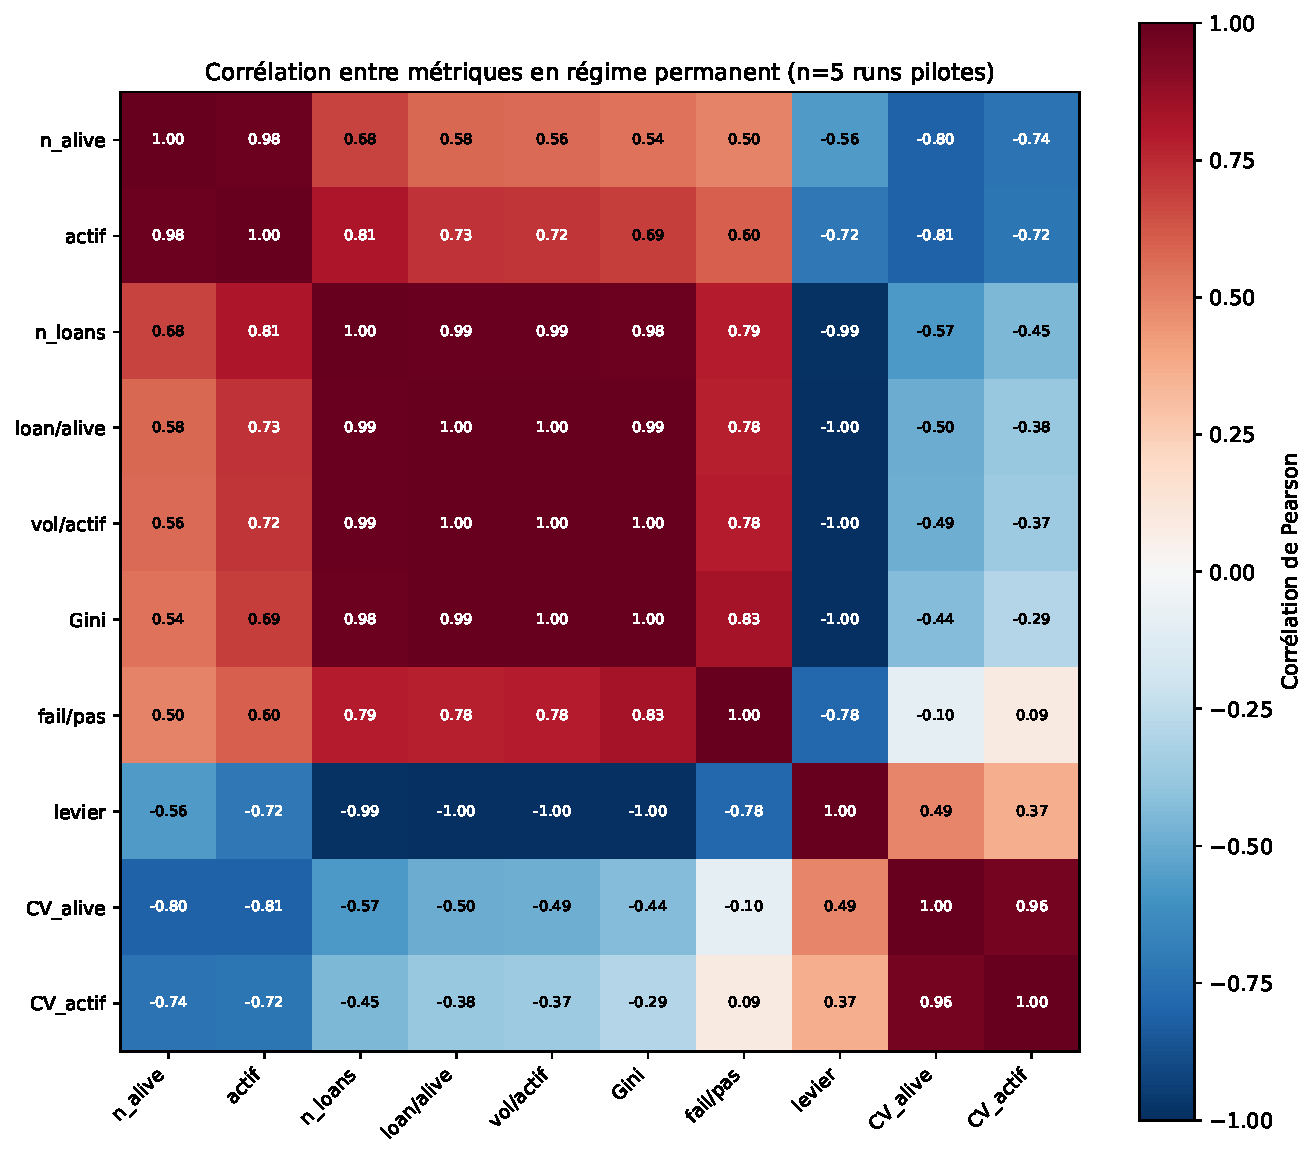
\includegraphics[width=0.92\linewidth]{figures/pilot_correlations.pdf}
  \caption{Correlations du pilote initial. Cette figure justifie de suivre
  simultanement \(n_{\mathrm{alive}}\), actif total, prets, densite financiere,
  faillites et Gini, plutot que de choisir une seule variable de taille.}
  \label{fig:pilot-corr}
\end{figure}

\section{Seuil en \(k\) et plateau}

Le parametre \(k=\texttt{n\_candidats\_pool}\) controle la rencontre sur le
marche du credit. Dans le cas homogene statique
\((\alpha_{\min}=\alpha_{\max}=1, \sigma_\alpha=0)\), \(k=3\) est
sous-critique a 1500--3000 pas : le reseau reste trop peu dense ou entre trop
tard dans une dynamique de faillites. \(k=4\) franchit un seuil et installe un
regime dense. Aux grands \(k\), la densite financiere ne croit pas
indefiniment : elle forme un plateau.

\begin{table}[H]
\centering
\begin{tabular}{rrrr}
\toprule
\(k\) & $\mathcal{B}$/3 seeds & $d_f$ moyen & \(n_{\mathrm{alive}}\) moyen \\
\midrule
2  & 0/3 & 0.015 & croissance forte \\
3  & 0/3 & 0.049 & croissance forte \\
4  & 3/3 & 0.399 & \(\approx 415\) \\
5  & 3/3 & 0.411 & \(\approx 330\) \\
20 & 3/3 & 0.380 & \(\approx 300\) \\
50 & 3/3 & 0.375 & \(\approx 325\) \\
\bottomrule
\end{tabular}
\caption{Lecture compacte du balayage \(k\), \(\epsilon=10^{-3}\), 1500 pas.}
\end{table}

\begin{figure}[H]
  \centering
  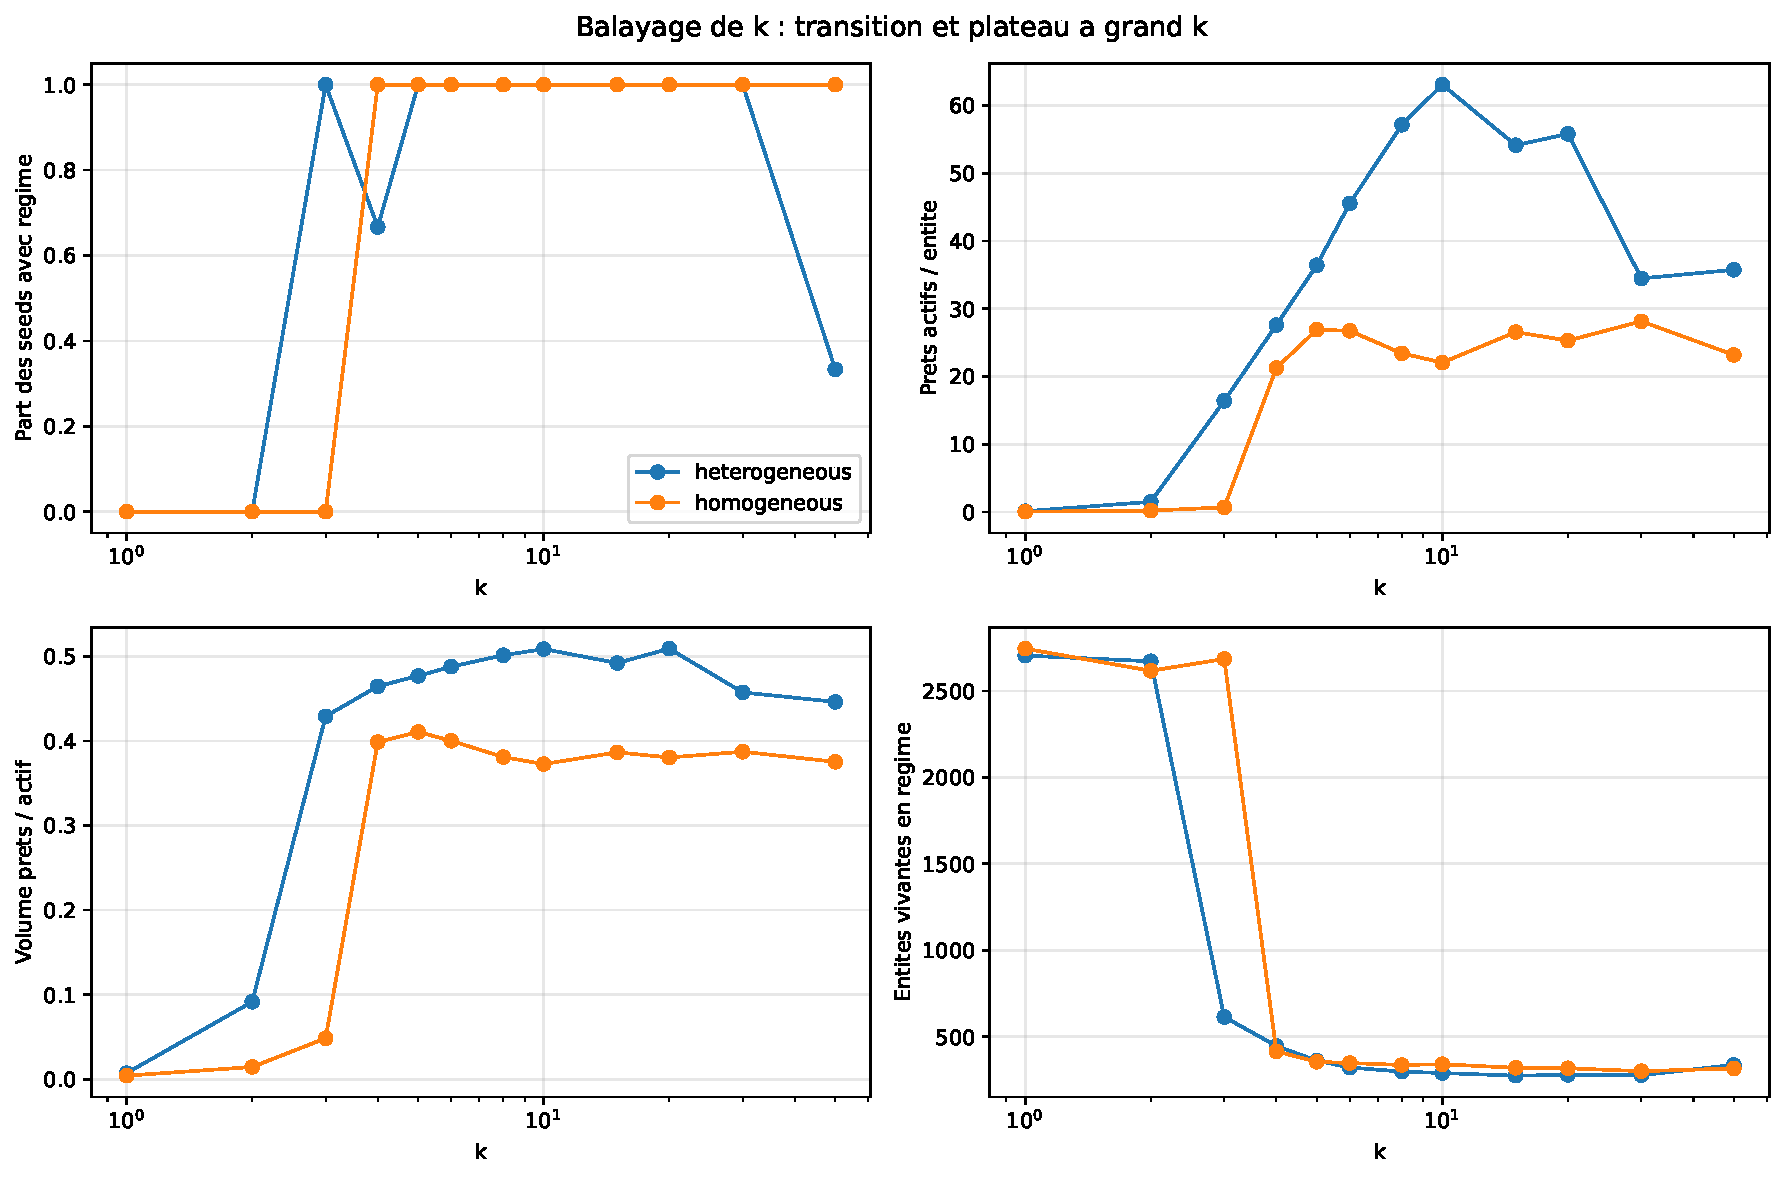
\includegraphics[width=0.95\linewidth]{figures/k_sweep_steps1500_eps0.001.pdf}
  \caption{Transition et plateau lorsque \(k\) augmente.
  Axe X : $k$ (\texttt{n\_candidats\_pool}), homogene statique
  ($\sigma_\alpha = 0$, $\epsilon = 10^{-3}$, 1\,500 pas, 3 seeds).
  Axe Y gauche : fraction de seeds a queue bornee (\(\mathcal{B}\)).
  Axe Y droit : densite financiere moyenne \(d_f = V/A\).
  La transition seuil $k=3\to4$ est nette ; la densite forme un plateau
  pour $k\ge4$.}
\end{figure}

\section{Resolution numerique \(\epsilon\)}

\(\epsilon\) est un parametre numerique, mais il agit fortement sur le nombre de
contrats. La conclusion robuste est double :
\begin{itemize}
  \item \(\epsilon=10^{-3}\) conserve les volumes financiers dans les points de
  reference tout en accelerant les campagnes ;
  \item \(\epsilon=10^{-2}\) change qualitativement le modele : le reseau dense
  disparait et la densite financiere tombe vers zero.
\end{itemize}

La densite en nombre de prets est donc une metrique mixte : elle decrit a la
fois la topologie economique et la resolution des micro-credits. Le volume
financier \(V/A\) est plus robuste.

\begin{figure}[H]
  \centering
  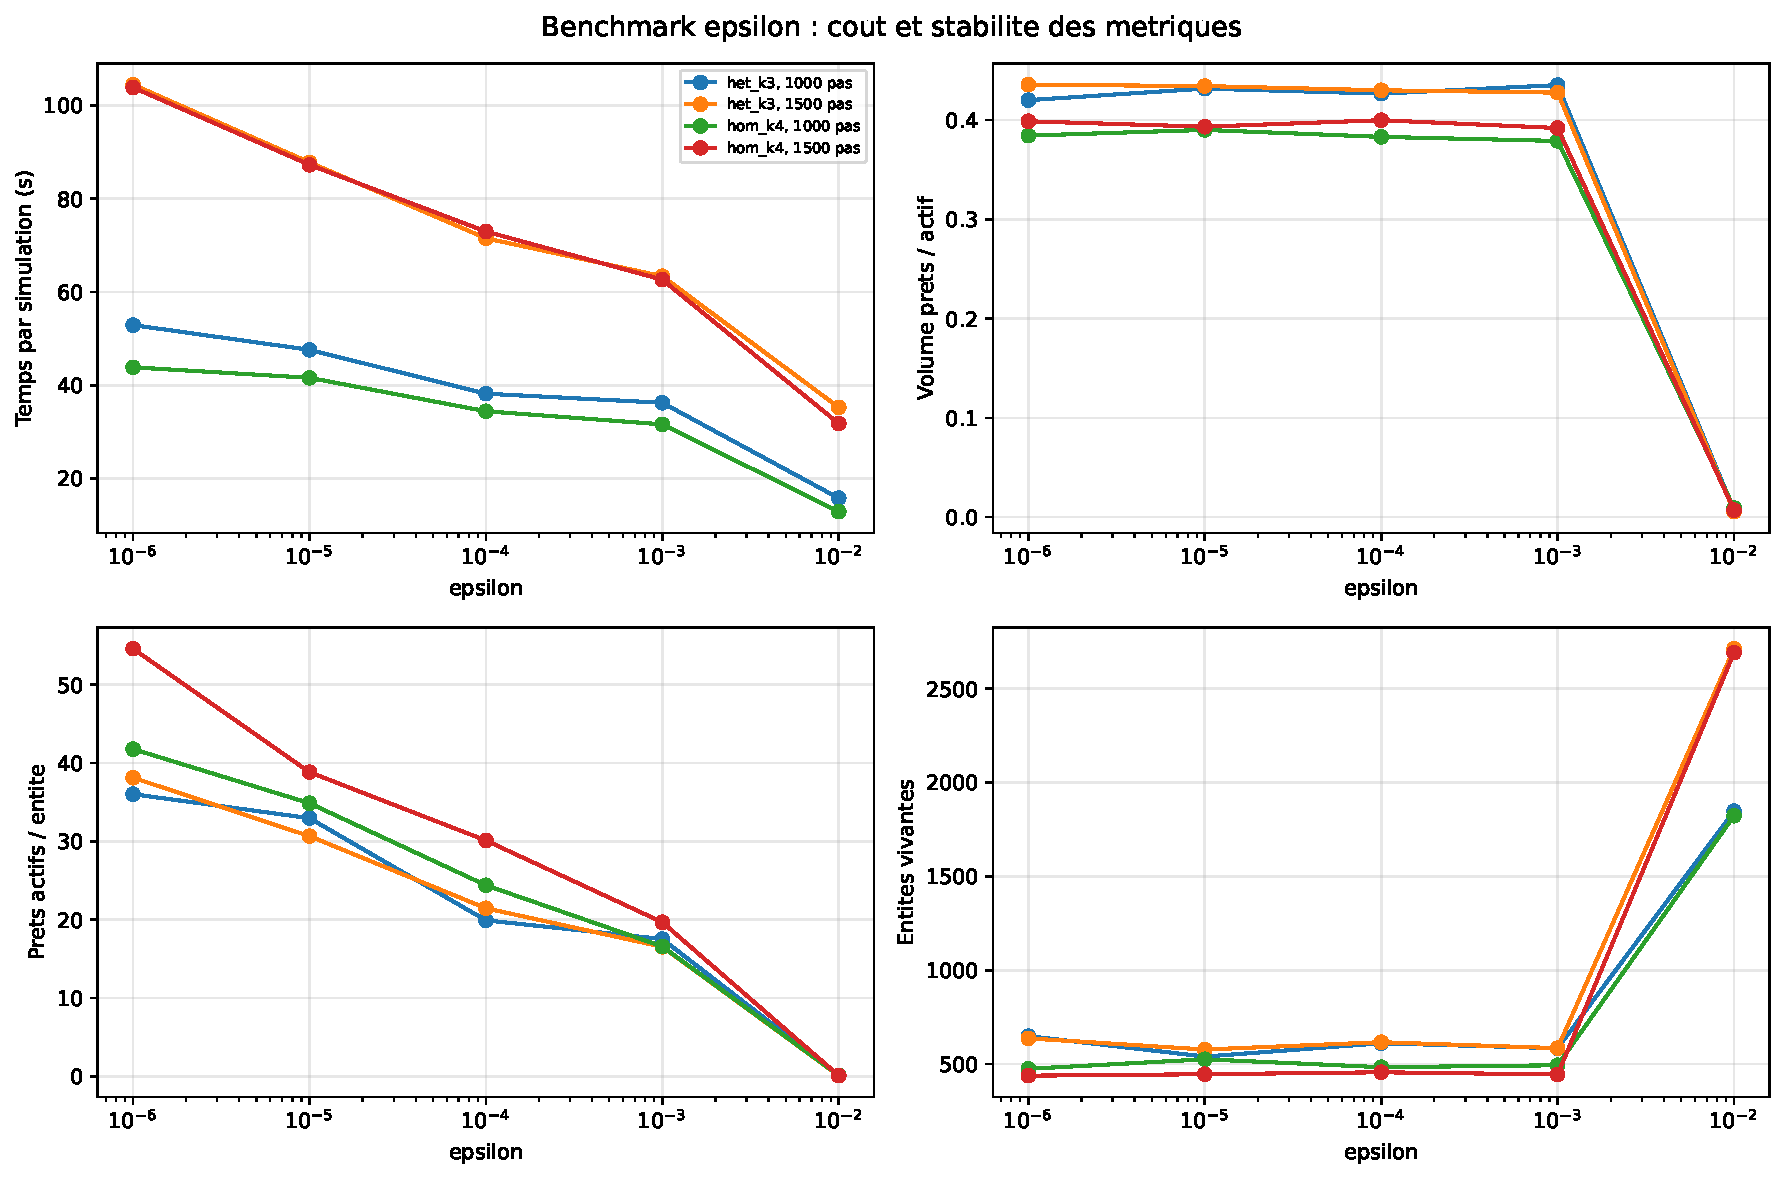
\includegraphics[width=0.95\linewidth]{figures/epsilon_runtime_probe.pdf}
  \caption{Compromis cout / stabilite des metriques lorsque \(\epsilon\) varie.}
\end{figure}

\section{Volatilite brownienne de \(\alpha\)}

Le cas principal reste homogene a la naissance :
\(\alpha_{\min}=\alpha_{\max}=1\). En revanche, \(\sigma_\alpha\) introduit une
dispersion dynamique. Elle joue un role de declencheur quand \(k=3\). Pour
\(k=3\), une fenetre active \(\sigma_\alpha\approx0.005\)--0.02 cree un reseau
dense. Une volatilite trop forte, \(\sigma_\alpha=0.05\) ou 0.1, detruit a
nouveau le volume financier. Pour \(k=4\), le regime existe deja a
\(\sigma_\alpha=0\), puis la densite augmente jusqu'a environ 0.02 avant de se
fragmenter.

\begin{figure}[H]
  \centering
  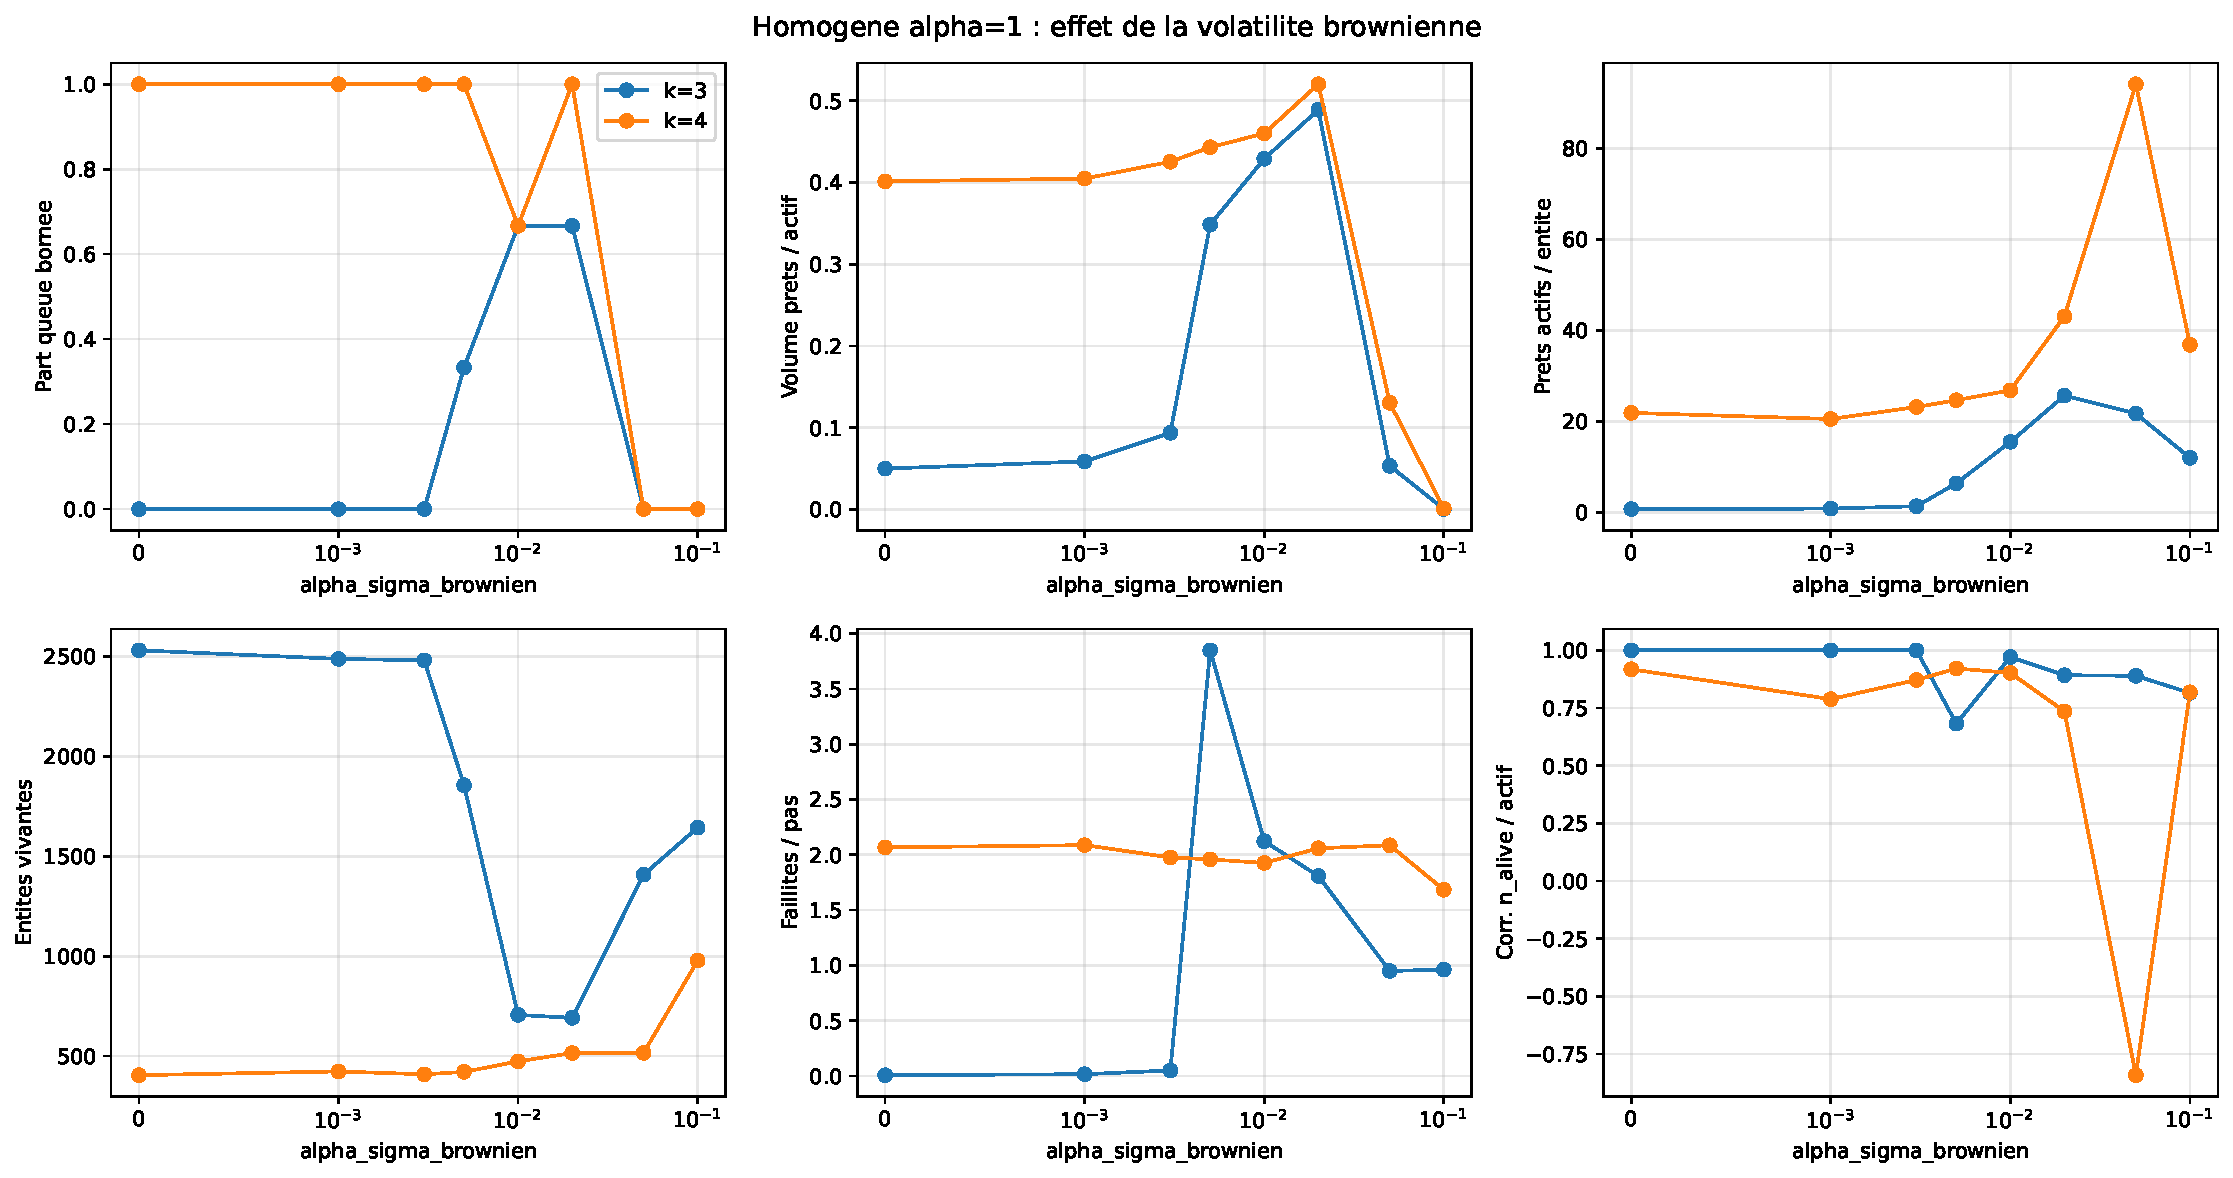
\includegraphics[width=0.95\linewidth]{figures/alpha_sigma_sweep_steps1500_eps0.001.pdf}
  \caption{Fenetre active de volatilite brownienne en alpha homogene.}
\end{figure}

\section{OAT autour de deux centres}

La campagne OAT Codex utilise deux centres :
\begin{itemize}
  \item \texttt{subcritical\_k3} : \(k=3\), \(\sigma_\alpha=0\), \(\epsilon=10^{-3}\) ;
  \item \texttt{regime\_k4} : \(k=4\), \(\sigma_\alpha=0\), \(\epsilon=10^{-3}\).
\end{itemize}

Quinze axes ont ete explores, hors amortissement. Pour
\texttt{actif\_liquide\_initial}, le passif inne initial a ete ajuste afin de
conserver une richesse nette initiale coherente de 10.

\begin{figure}[H]
  \centering
  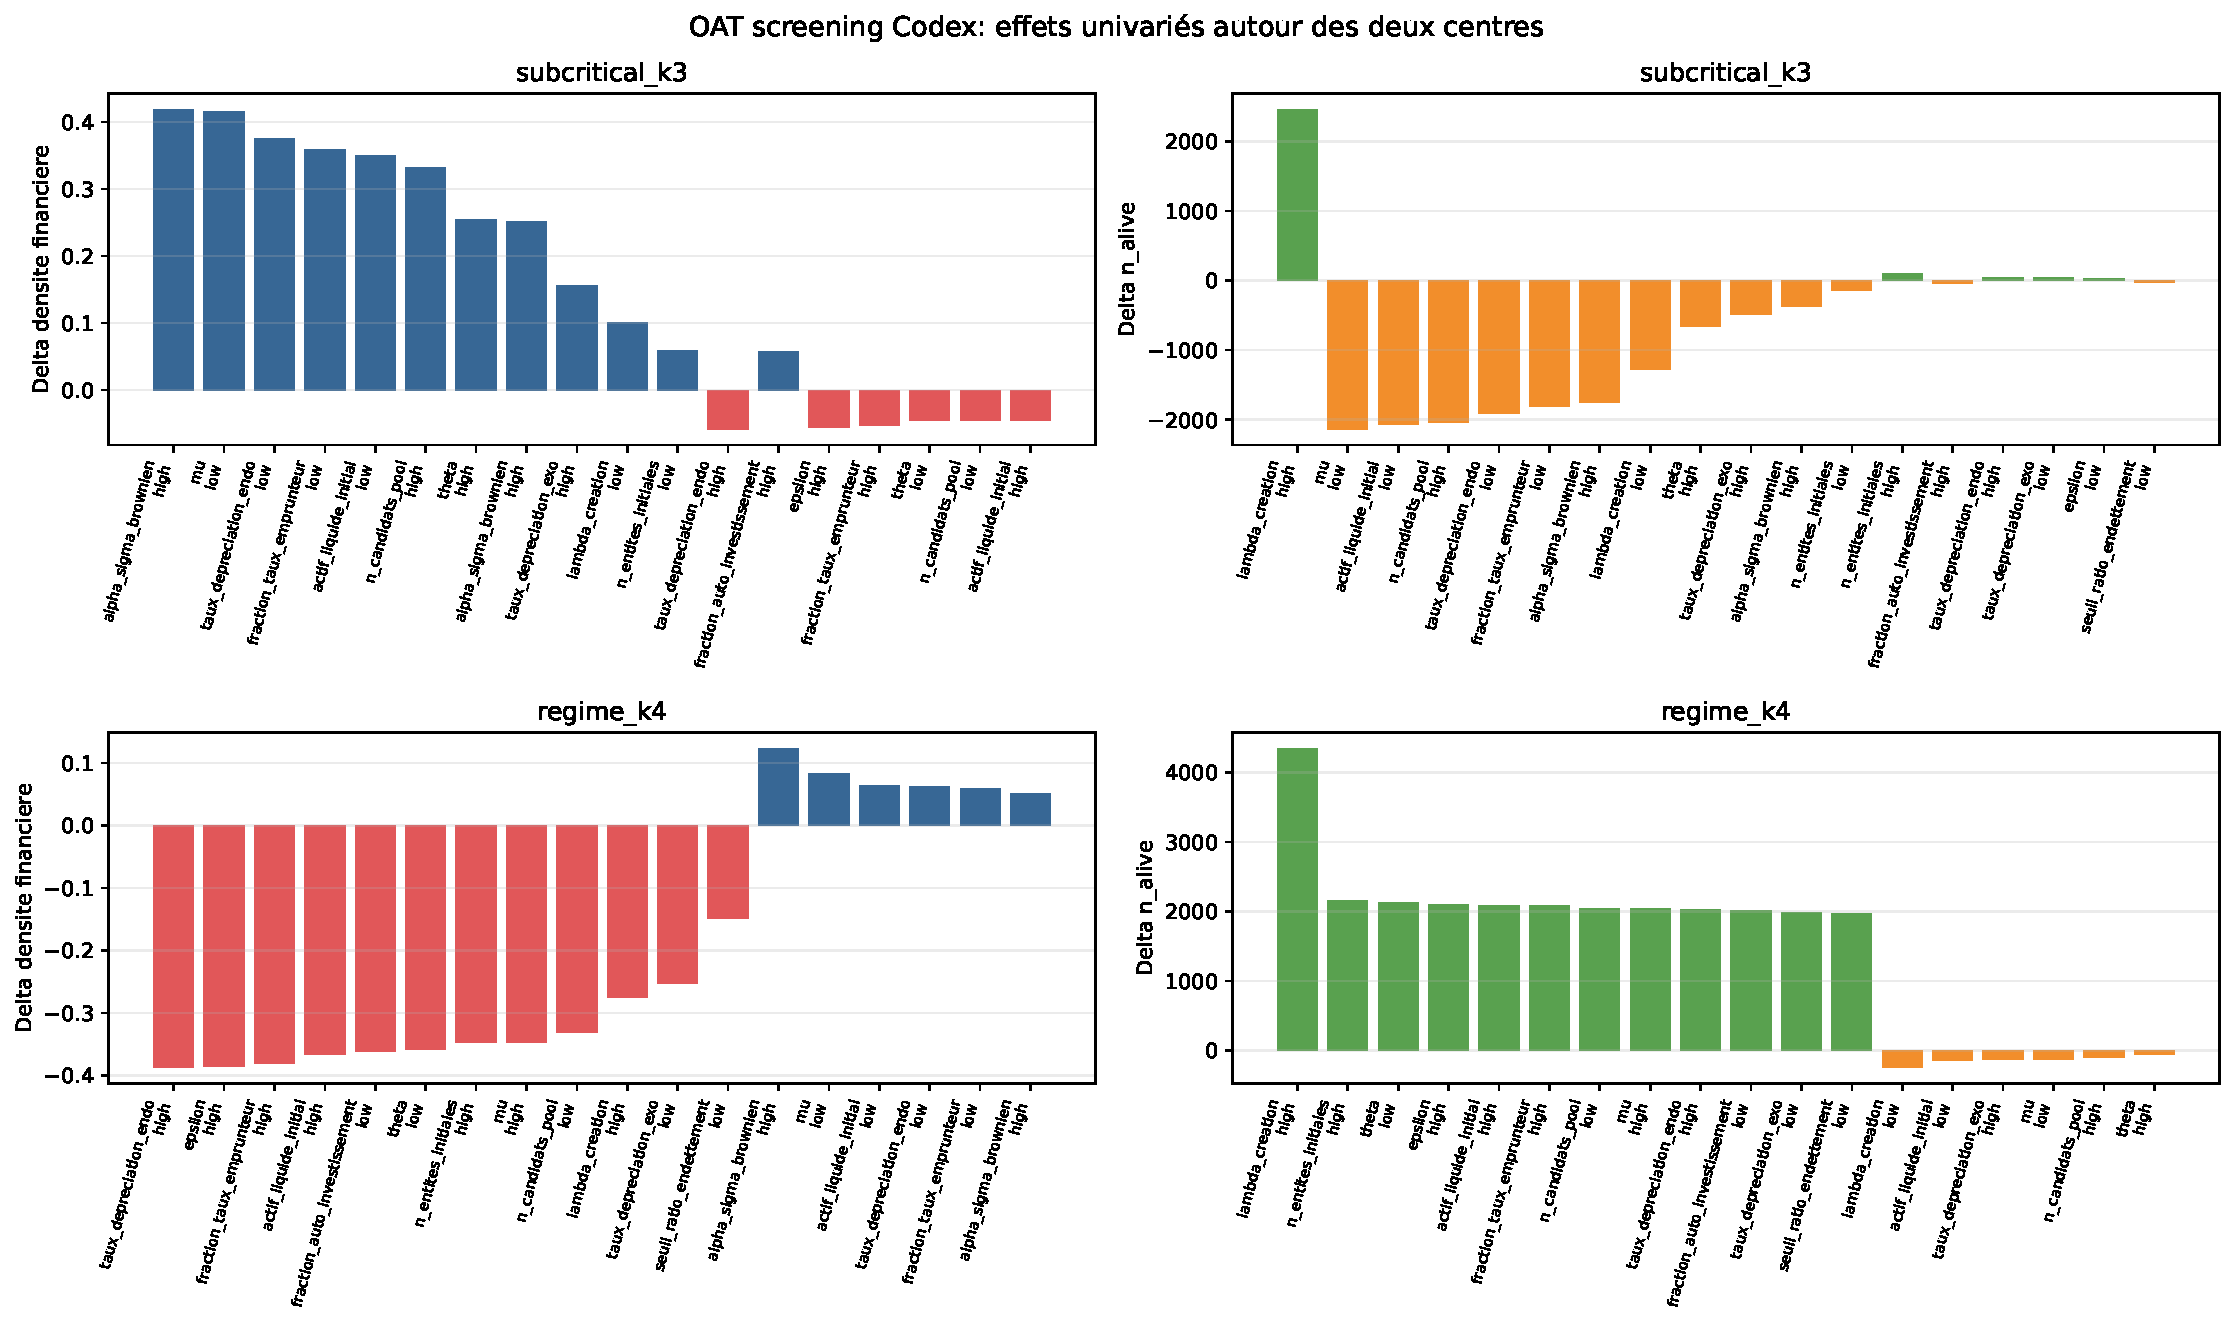
\includegraphics[width=0.98\linewidth]{figures/codex_oat_screen_steps1500_seeds42.pdf}
  \caption{Effets OAT autour des deux centres (seed 42, 1\,500 pas,
  $\epsilon=10^{-3}$). Chaque barre est un $\Delta d_f$ (delta de densite
  financiere $V/A$) par rapport au centre $C_3$ (groupe gauche) ou $C_4$
  (groupe droit). La couleur indique si la queue est bornee ($\mathcal{B}$)
  ou non.}
\end{figure}

\begin{table}[H]
\centering
\small
\begin{tabularx}{\linewidth}{lXX}
\toprule
Centre & Parametres qui densifient & Parametres qui detruisent ou retardent \\
\midrule
\(k=3\) & \(\sigma_\alpha=0.02\), \(\mu=0\), \(\delta_{\mathrm{endo}}=0.02\),
\(f=0\), actif initial 100, \(k=4\), \(\theta=0.5\)
& \(\epsilon=10^{-2}\), \(\delta_{\mathrm{endo}}=0.1\), \(\theta=0.2\),
\(\mu=0.1\) \\
\(k=4\) & \(\sigma_\alpha=0.02\), \(\mu=0\), actif initial 100,
\(f=0\), \(k=5\)
& \(\delta_{\mathrm{endo}}=0.1\), \(\epsilon=10^{-2}\), \(f=0.5\),
actif initial 400, \(\phi=0.25\), \(\theta=0.2\), \(\lambda=4\) \\
\bottomrule
\end{tabularx}
\caption{Lecture qualitative de l'OAT seed 42. \(f\) est
\texttt{fraction\_taux\_emprunteur} et \(\phi\) est
\texttt{fraction\_auto\_investissement}.}
\end{table}

\section{Sonde longue : ce qui etait trop court a 1500 pas}

Plusieurs simulations a 1500 pas etaient ambigues. La sonde longue a relance
8 cas a 3000 pas. Elle montre que certains cas entraient seulement dans une
phase dense, sans etre encore bornes.

\begin{table}[H]
\centering
\begin{tabular}{lrrrr}
\toprule
Cas & $\mathcal{B}$ & $d_f$ & \(n_{\mathrm{alive}}\) & pente rel. \(n\) \\
\midrule
\texttt{k3\_sigma0005} & non & 0.404 & 716 & +0.295 \\
\texttt{k3\_sigma002} & non & 0.494 & 722 & +0.041 \\
\texttt{k3\_theta05} & oui & 0.387 & 598 & -0.154 \\
\texttt{k3\_mu0} & oui & 0.508 & 382 & +0.139 \\
\texttt{k4\_depr\_endo002} & oui & 0.488 & 444 & +0.033 \\
\texttt{k4\_theta02} & non & 0.022 & 5010 & +0.494 \\
\texttt{k4\_actif400} & non & 0.017 & 4898 & +0.484 \\
\texttt{k4\_lambda4} & non & 0.079 & 9424 & +0.507 \\
\bottomrule
\end{tabular}
\caption{Sonde longue 3000 pas, seed 42. La ligne \(k=3,\sigma=0.005\) confirme
que l'entree visible vers 1200 pas n'etait pas encore un regime etabli.}
\end{table}

\begin{figure}[H]
  \centering
  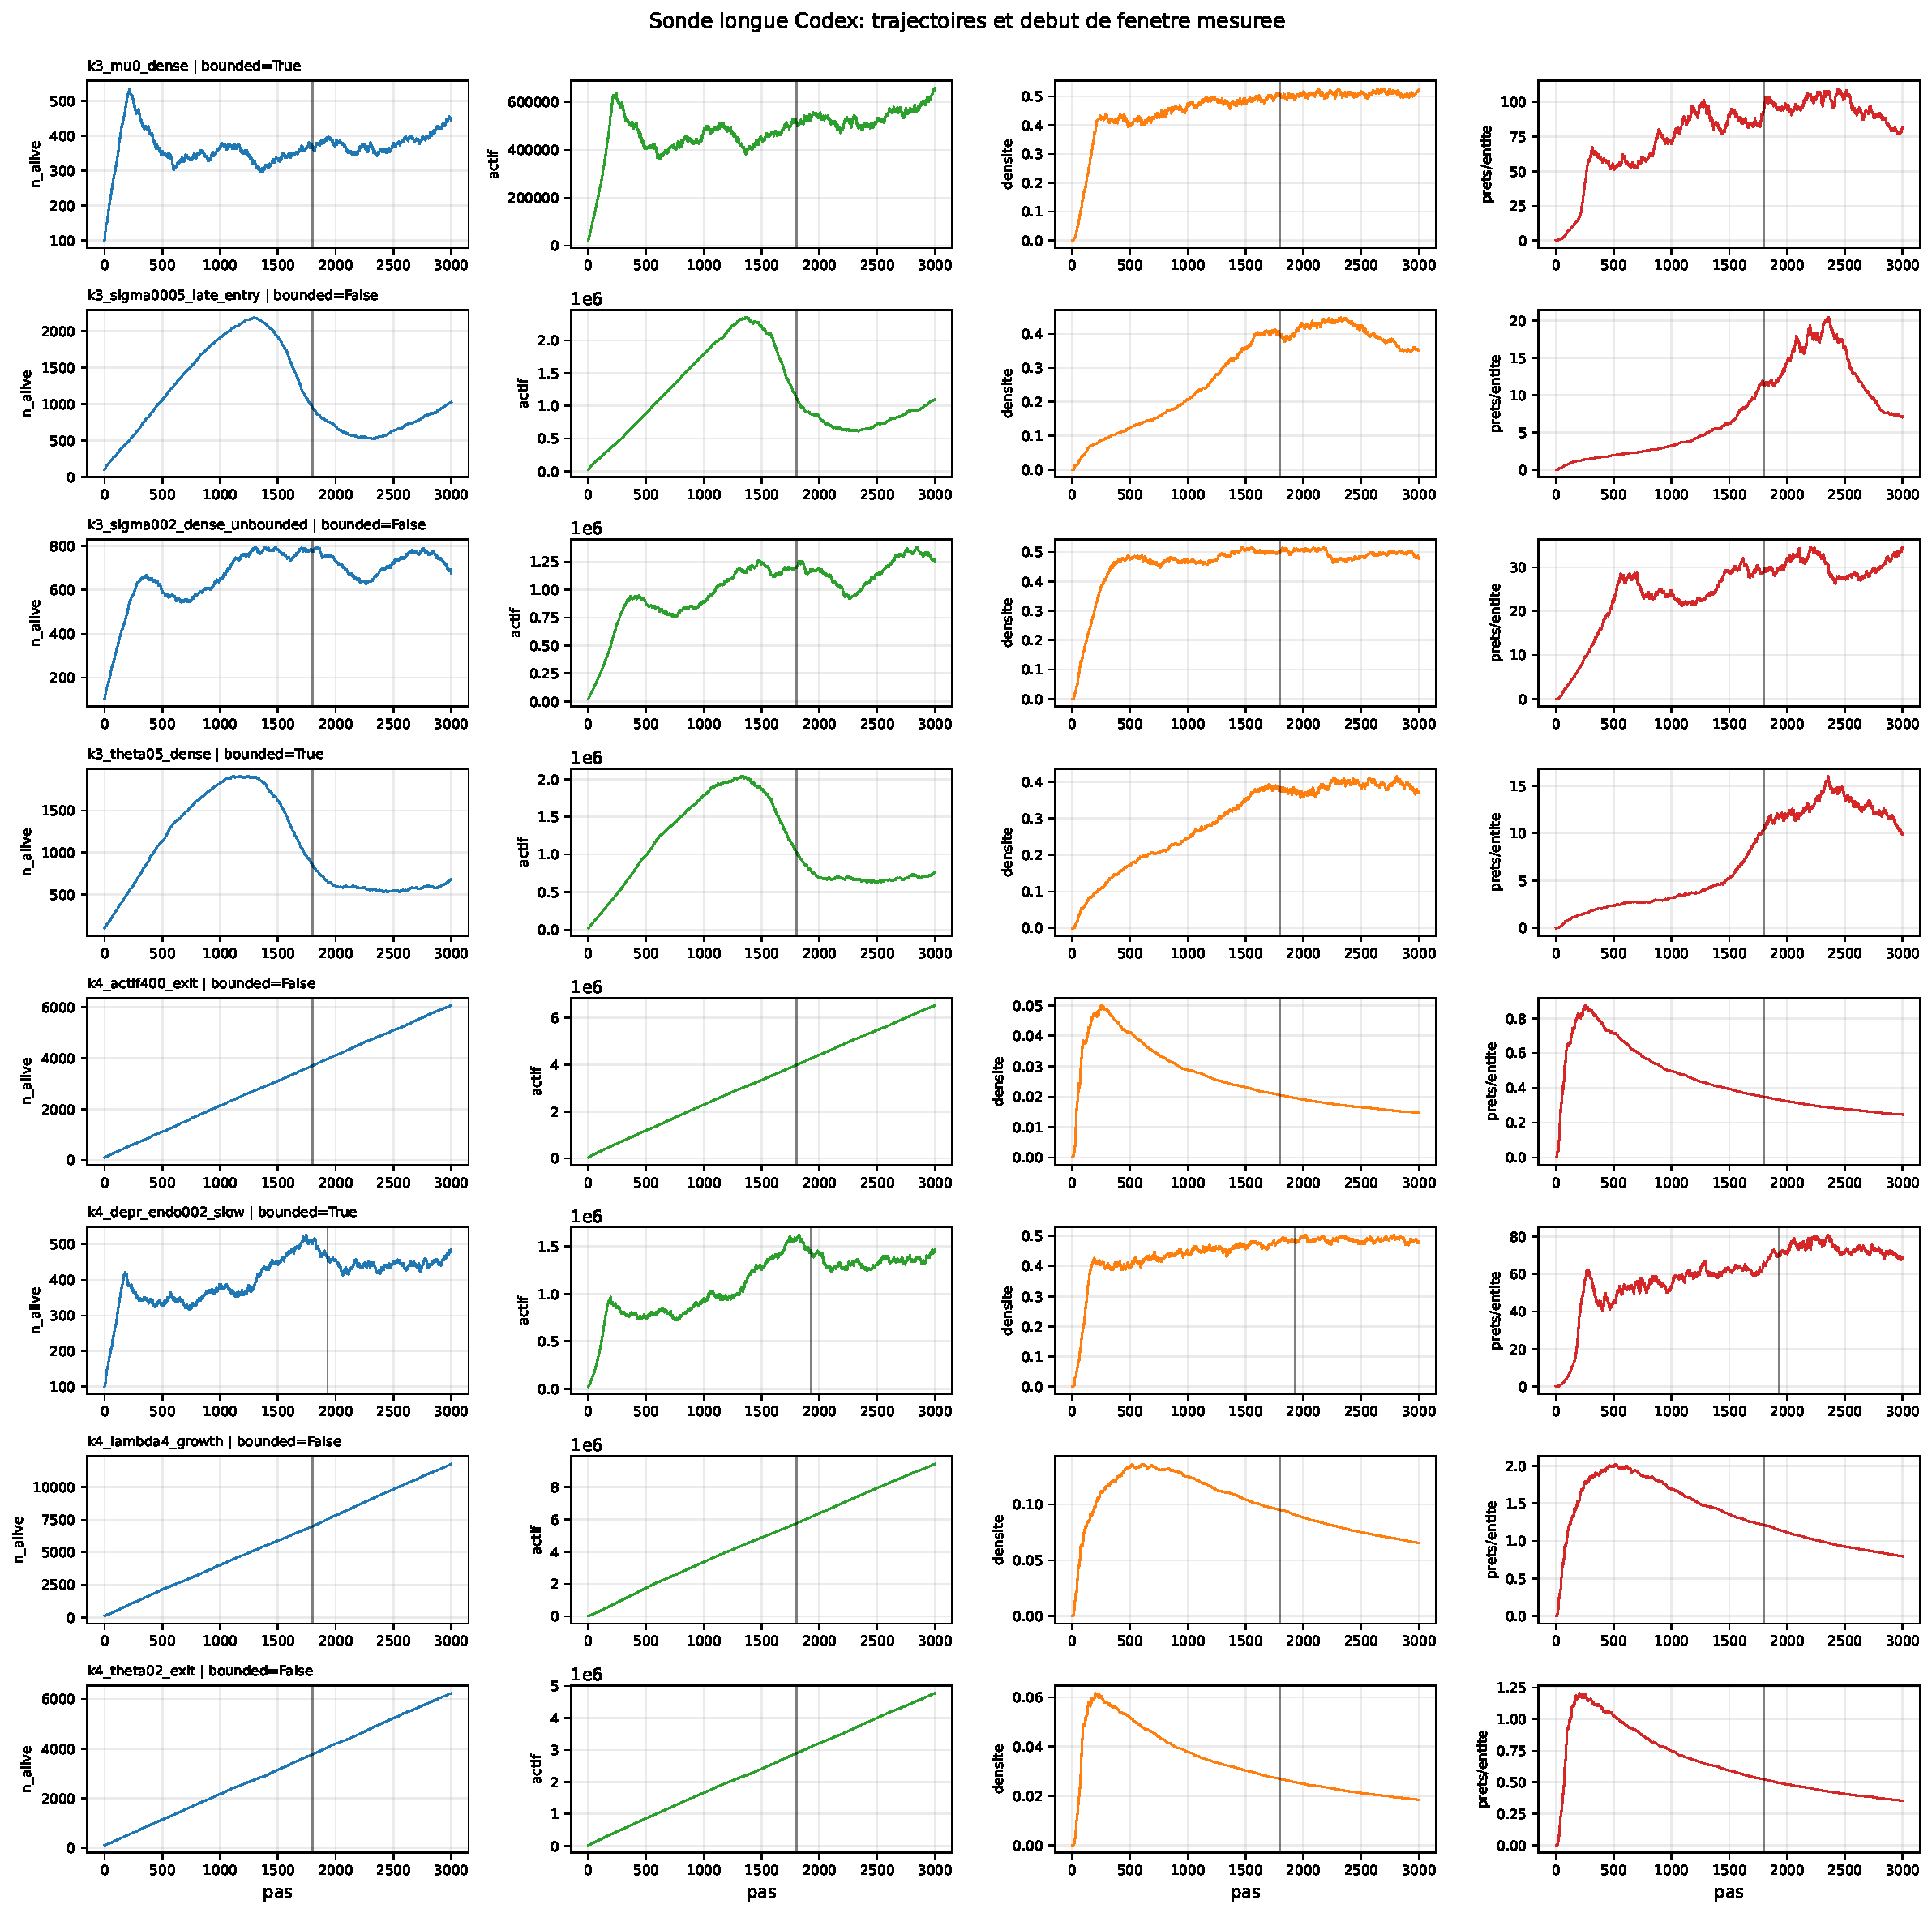
\includegraphics[width=0.98\linewidth]{figures/codex_long_probe_steps3000_seeds42.pdf}
  \caption{Sonde longue 3\,000 pas, seed 42 -- trajectoires des 8 cas ambigus.
  Quatre colonnes par cas :
  (1) bleu : $n_{\mathrm{alive}}$ ;
  (2) vert : actif total $A$ ;
  (3) orange : densite financiere en volume $d_f = V/A$
    (\texttt{densite\_fin}) ;
  (4) rouge : densite contractuelle $\ell = L/n_{\mathrm{alive}}$
    (\texttt{n\_prets/n\_alive}).
  La ligne verticale indique le debut de la fenetre de mesure
  (\(\approx 0.6 \times T\)).}
\end{figure}

\begin{figure}[H]
  \centering
  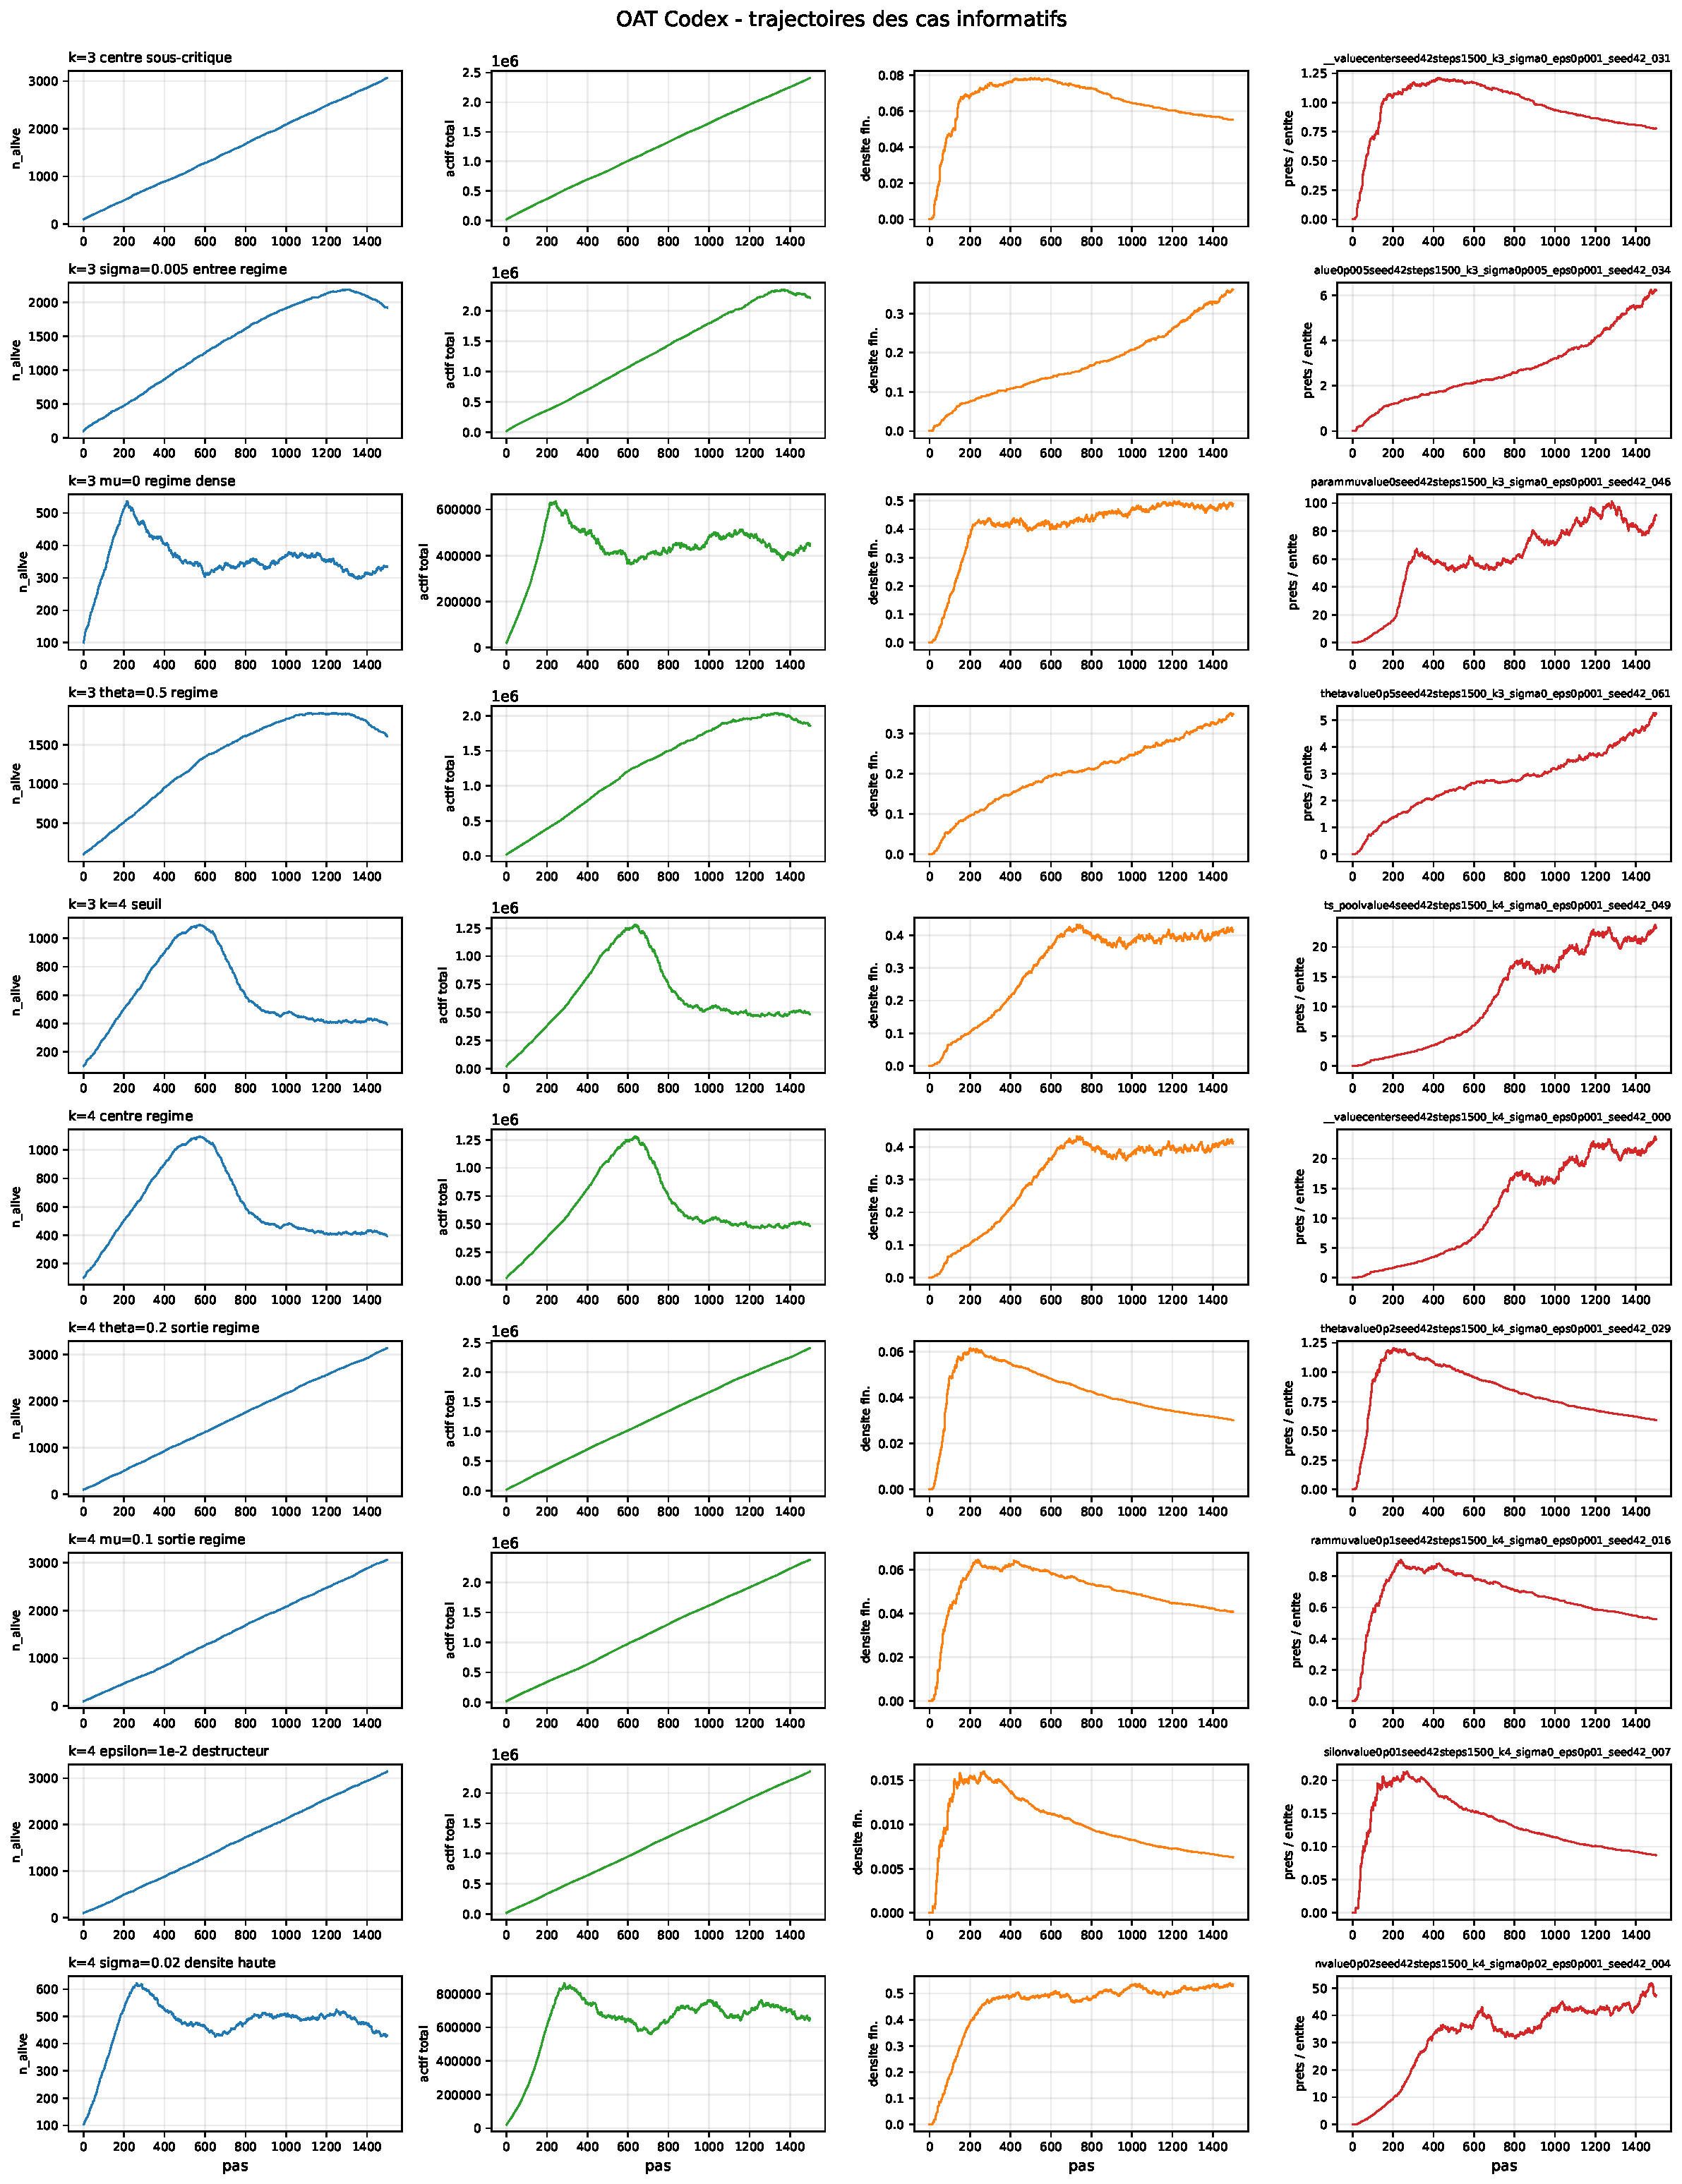
\includegraphics[width=0.98\linewidth]{figures/codex_oat_key_trajectories.pdf}
  \caption{Planches comparatives OAT visibles dans Simulation Lab.}
\end{figure}

\section{Prediction depuis les parametres}

Un test predictif simple a ete fait sur 193 observations issues des pilotes,
sweeps \(k\), sweeps \(\sigma_\alpha\), benchmark \(\epsilon\), sonde guidee et
OAT. Les variables explicatives sont les parametres de simulation, incluant
\(k\), \(\sigma_\alpha\), \(\theta\), \(\mu\), \(\lambda\), les depreciations,
la dotation initiale, \(\epsilon\) et l'ecart \(\alpha_{\max}-\alpha_{\min}\).

Les resultats en validation croisee sont :
\begin{itemize}
  \item prediction de \texttt{bounded\_tail} : accuracy 0.845, balanced accuracy
  0.840 ;
  \item prediction de la densite financiere : \(R^2=0.584\), RMSE 0.122 ;
  \item prediction de \(\log(1+n_{\mathrm{alive}})\) : \(R^2=0.605\), RMSE 0.548.
\end{itemize}

La classification du regime est donc deja assez predictable. Les regressions
restent plus difficiles car les effets sont non lineaires, avec seuils et
plateaux.

\begin{figure}[H]
  \centering
  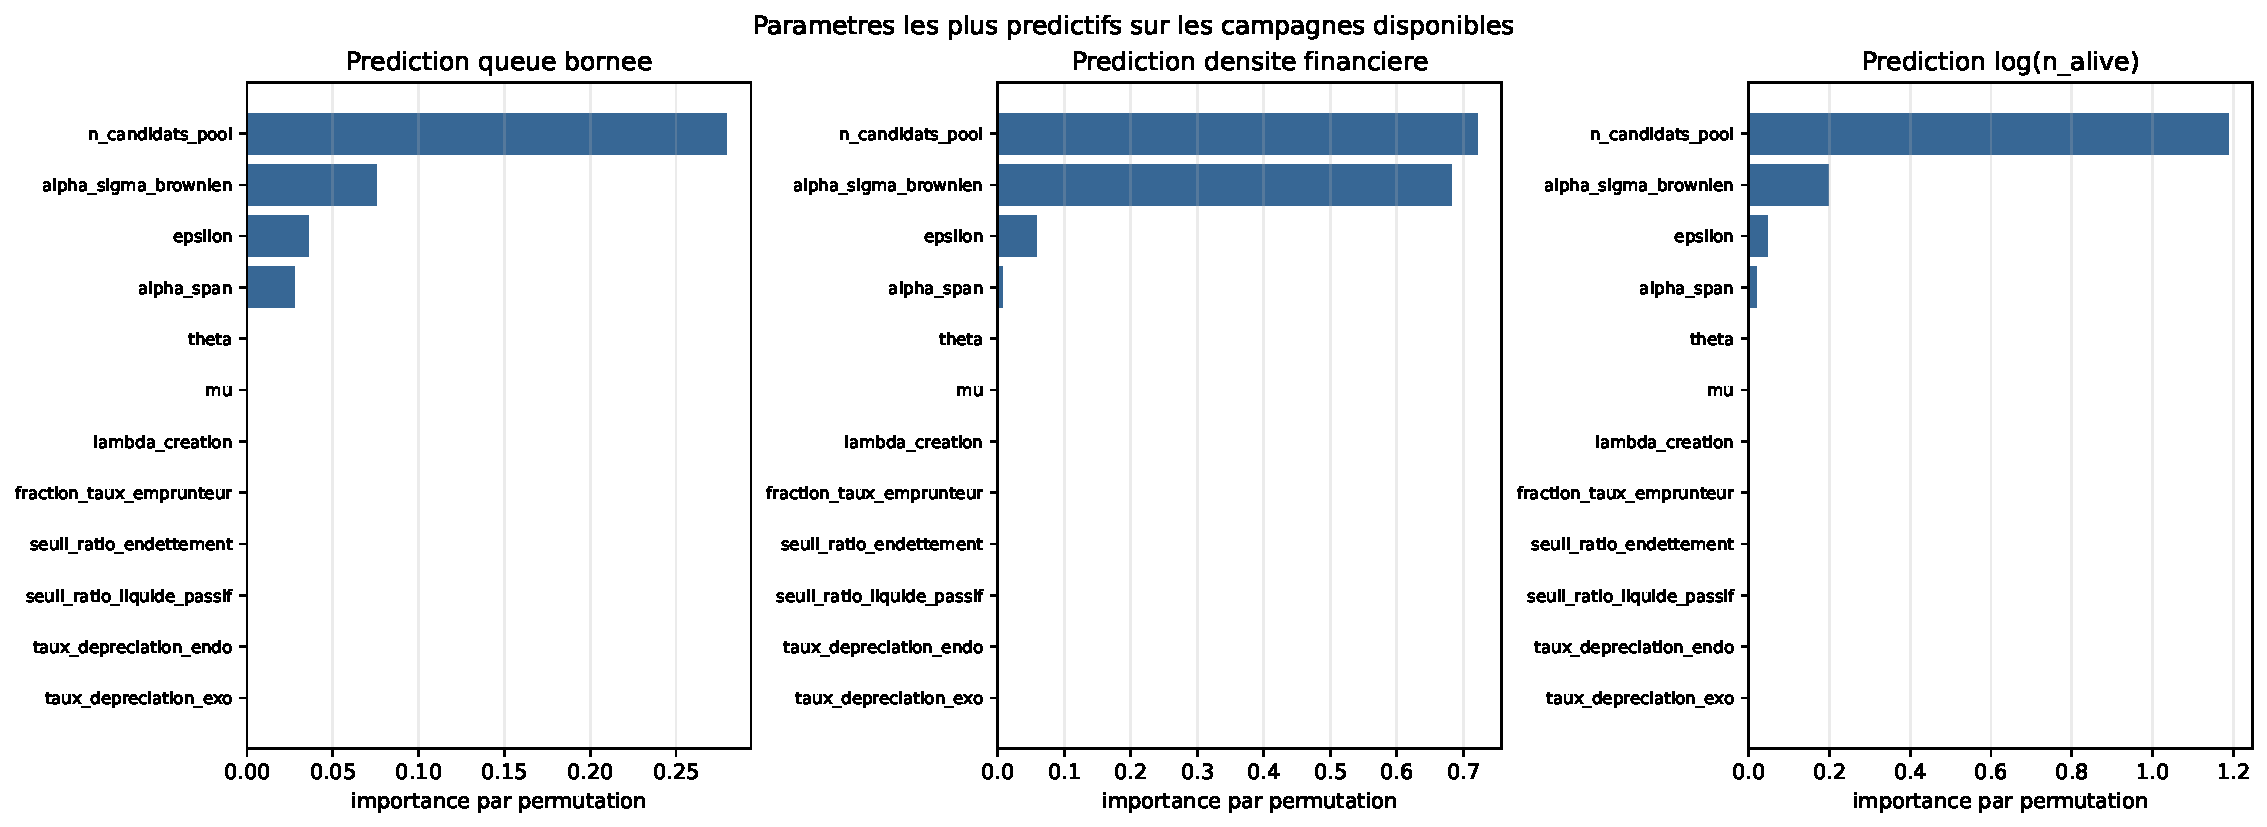
\includegraphics[width=0.98\linewidth]{figures/codex_predictive_importance.pdf}
  \caption{Importance predictive des parametres par permutation.}
\end{figure}

\begin{figure}[H]
  \centering
  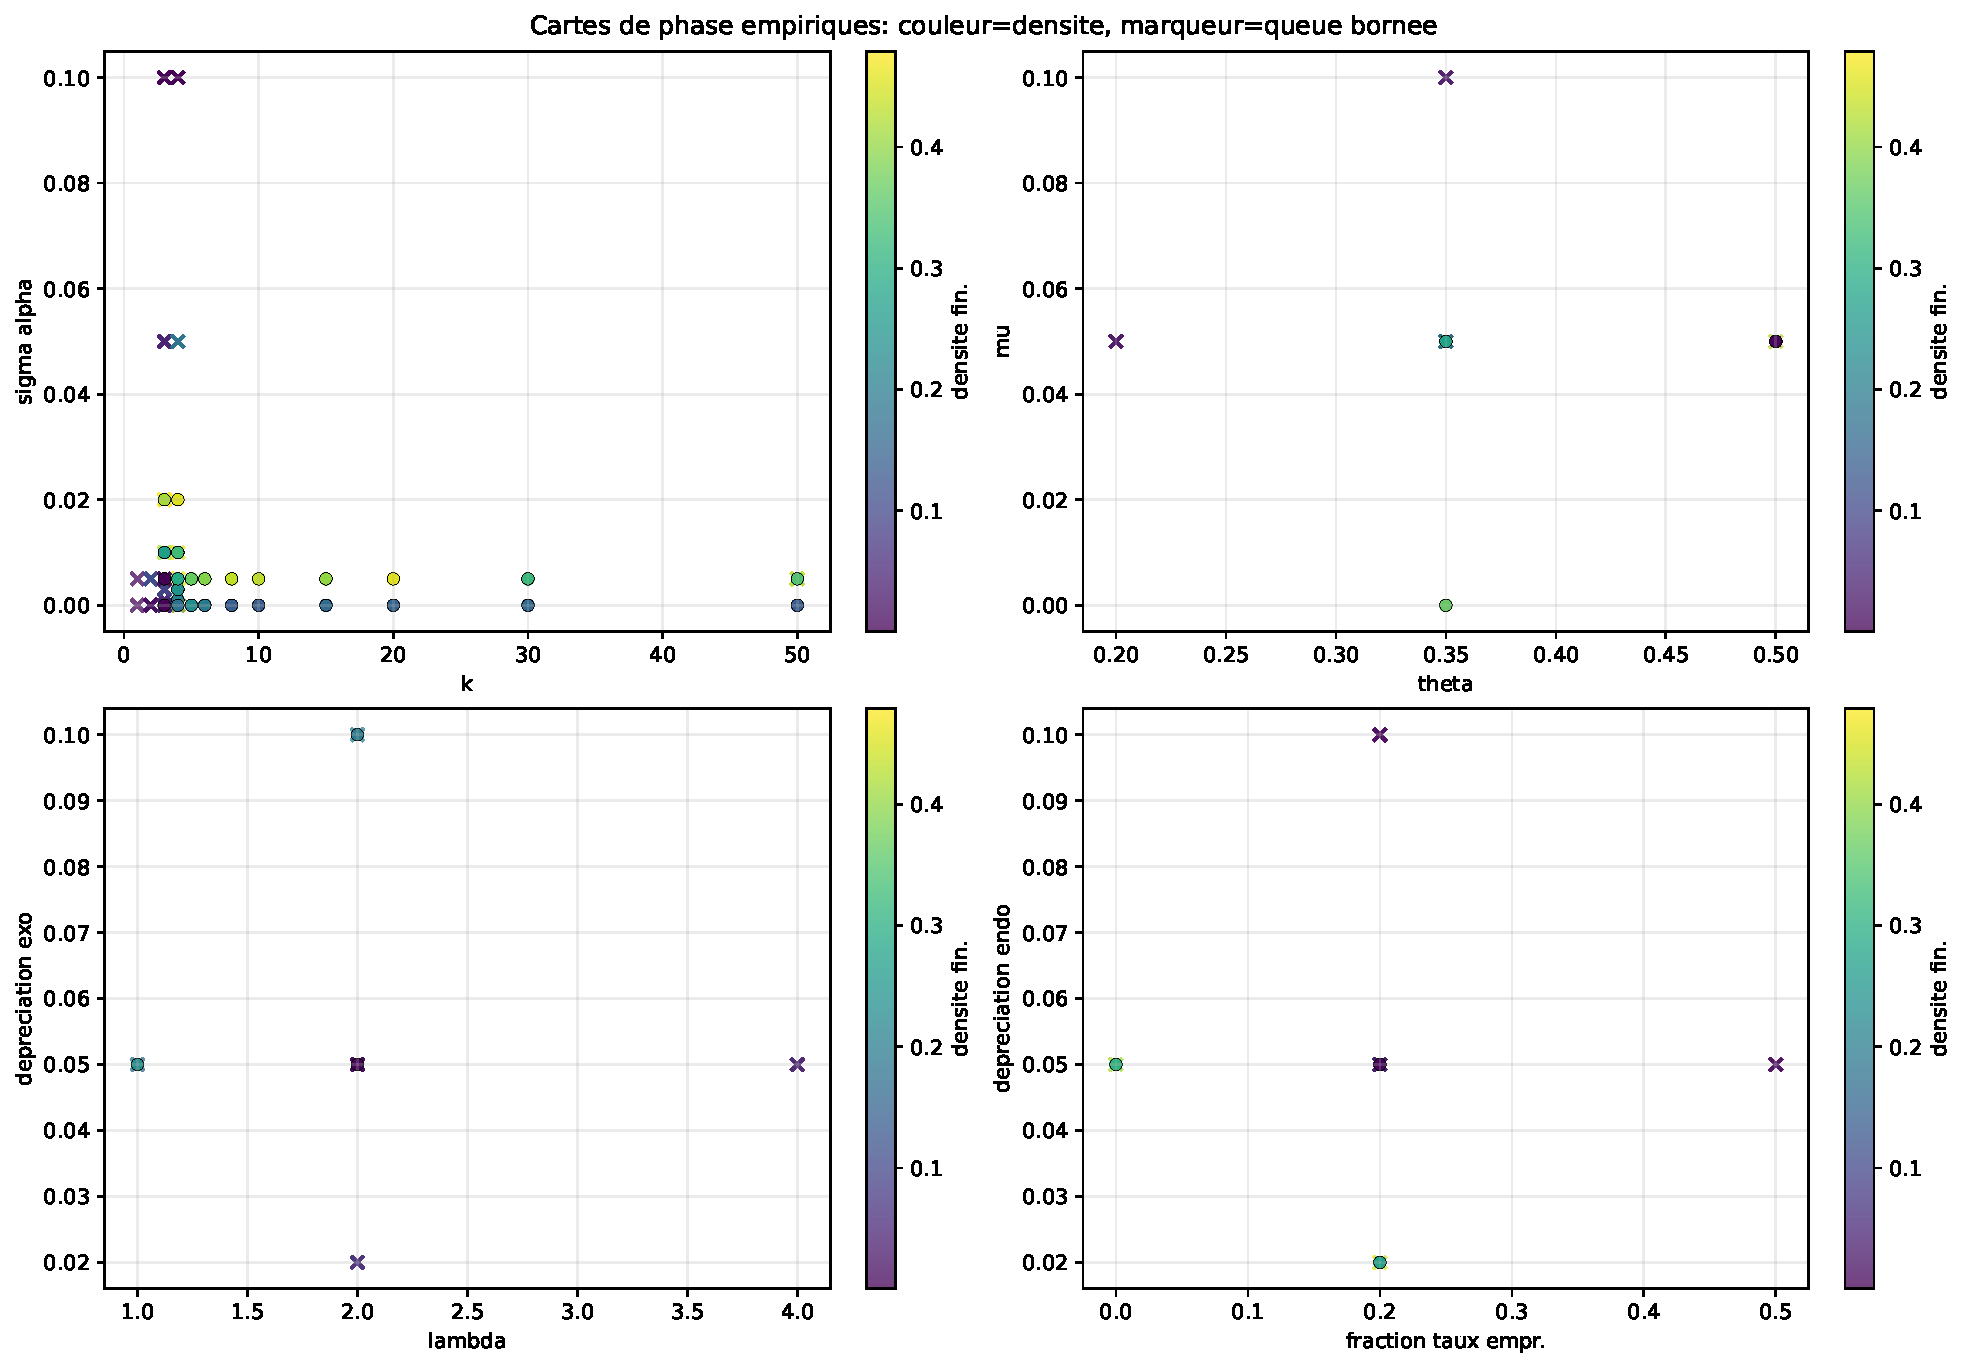
\includegraphics[width=0.98\linewidth]{figures/codex_phase_maps.pdf}
  \caption{Cartes de phase empiriques. Les marqueurs ronds sont les cas a queue
  bornee ; les croix les cas non bornes. La couleur indique la densite
  financiere.}
\end{figure}

\section{Decorrelation \(n_{\mathrm{alive}}\) / actif}

Le nombre d'entites et l'actif total ne mesurent pas la meme chose. Dans une
croissance non financee, ils montent souvent ensemble : les correlations de
queue peuvent etre proches de 1, mais ce n'est pas un signe de regime. Dans un
regime dense, les faillites peuvent stabiliser \(n_{\mathrm{alive}}\) alors que
l'actif moyen des survivants continue de se reorganiser. Le cas historique
\(k=4, \sigma_\alpha=0.05, \epsilon=10^{-3}\) illustre cette decorrelation :
\(n_{\mathrm{alive}}\) peut rester borne alors que l'actif et le volume de prets
portent encore une derive ou une fragmentation en micro-credits.

L'interpretation pratique est la suivante :
\begin{itemize}
  \item une forte correlation positive \(n/A\) en queue peut signaler une
  croissance commune non stabilisee ;
  \item une correlation faible ou negative n'est pas necessairement une
  anomalie : elle peut signaler une population stabilisee mais une composition
  du bilan encore mobile ;
  \item il faut donc predire au moins deux sorties : la taille demographique et
  la taille bilancielle.
\end{itemize}

\section{Iterations du protocole}

L'etude s'est deroulee en cinq grandes phases iteratives.

\textbf{Phase 1 -- Pilote et criteres (boucles 1--4).}
Le critere de convergence initial (chute de 25\,\% de \(n_{\mathrm{alive}}\))
a ete remplace par des diagnostics de queue combinant pentes relatives et
IQR (voir section~\ref{sec:critere-regime}). Le seuil en \(k\) (transition
3$\to$4 en regime homogene) et la resolution numerique \(\epsilon\) ont ete
identifies lors des premiers balayages 1D.

\textbf{Phase 2 -- OAT a deux centres (boucles 5--10).}
62 simulations OAT autour de $C_3$ et $C_4$, puis validation sur 3 seeds.
Les parametres les plus impactants ont ete classes en effets robustes
(meme sens sur tous les seeds) et effets fragiles (dependants du seed).

\textbf{Phase 3 -- Couplages coarse (boucles 11--14).}
Quatre cartes de phase 2D a grille grossiere (3 seeds, 1\,500 pas) :
\(\lambda\times k\), \(k\times\mu\), \(\sigma_\alpha\times k\),
\(\theta\times\delta_{\mathrm{endo}}\). Ces cartes ont identifie les
interactions dominantes et les frontieres de regime.

\textbf{Phase 4 -- Probabilites et sondes longues (boucles 15--17).}
13 seeds supplementaires sur 7 cas limites ; extension de
$k=3,\sigma_\alpha=0.005$ a 10\,000 pas (convergence tardive confirmee).
Identification de deux parametres a effet nul (reliquefaction).

\textbf{Phase 5 -- Campagnes adaptatives (boucles 18--21).}
1\,479 runs au total sur quatre campagnes avec allocation adaptative
(3 seeds en zones stables, 15 aux frontieres) :
\(\lambda\times k\) (417), \(k\times\mu\) (327),
\(\sigma_\alpha\times k\) (267), \(\theta\times\delta\) unifie (468).
La campagne \(\theta\times\delta\) unifiee a mis en evidence un artefact
d'extinction (\(\delta\ge0.12\) : queue bornee par zero, non par regime).

\section{Balayage fin de \(\lambda\) comme variable continue}
\label{sec:lambda-fin}

Le parametre \(\lambda=\texttt{lambda\_creation}\) n'avait ete teste qu'aux
valeurs discretes \(\{1, 2, 4\}\). La sonde longue montrait que \(\lambda=4\)
reste en croissance a 3000 pas, mais la frontiere n'etait pas localisee. Un
balayage fin a ete conduit avec
\(\lambda\in\{1.0, 1.2, 1.4, 1.6, 1.8, 2.0, 2.5, 3.0, 3.5, 4.0, 5.0\}\),
trois seeds (42, 7, 123), \(\epsilon=10^{-3}\), 1500 pas, pour les deux centres
\(k=3\) et \(k=4\).

\subsection*{Resultats pour \(k=4\)}

\begin{table}[H]
\centering
\small
\begin{tabular}{rrrrrr}
\toprule
\(\lambda\) & $\mathcal{B}$/3s & $d_f$ (moy.$\pm$std) & \(n_{\mathrm{alive}}\) & note \\
\midrule
1.0 & 1/3 & \(0.423\pm0.009\) & 188 & transition \\
1.2 & 2/3 & \(0.411\pm0.001\) & 249 & transition \\
1.4 & 3/3 & \(0.406\pm0.004\) & 279 & \textbf{robuste} \\
1.6 & 3/3 & \(0.402\pm0.007\) & 318 & robuste \\
1.8 & 3/3 & \(0.403\pm0.010\) & 366 & robuste \\
2.0 & 3/3 & \(0.401\pm0.006\) & 405 & robuste \\
2.5 & 1/3 & \(0.393\pm0.002\) & 605 & instable \\
3.0 & 0/3 & \(0.384\pm0.002\) & 1105 & non borne, df encore eleve \\
3.5 & 0/3 & \(0.254\pm0.091\) & 3184 & effondrement partiel \\
4.0 & 0/3 & \(0.128\pm0.047\) & 4609 & effondrement \\
5.0 & 0/3 & \(0.051\pm0.003\) & 6114 & quasi-effondrement \\
\bottomrule
\end{tabular}
\caption{Balayage fin de \(\lambda\), centre \(k=4\), 1500 pas, 3 seeds.}
\end{table}

La frontiere robuste pour \(k=4\) se situe entre \(\lambda=2.0\) (3/3 bornes)
et \(\lambda=2.5\) (1/3 borne). La densite financiere reste elevee jusqu'a
\(\lambda=3.0\) (\(D\approx0.38\)) meme si la queue n'est plus bornee, ce
qui signifie que le reseau de credit se forme encore mais que le nombre
d'entites continue de croitre sans faillites compensatrices suffisantes.
Au-dela de \(\lambda\approx3.5\), la densite s'effondre : la croissance de
population est si forte que le reseau ne se densifie plus.

Un point notable : \(\lambda=1.0\) a 1/3 seeds bornes et une densite de 0.42.
Le systeme peut donc entrer en regime a tres faible taux de creation, mais la
petite population initiale le rend plus sensible aux fluctuations de seed.

\subsection*{Resultats pour \(k=3\)}

Aucune valeur de \(\lambda\) testee (\(1.0\) a \(5.0\)) ne produit de queue
bornee en homogene \(\sigma_\alpha=0\). La densite financiere decline
monotonement avec \(\lambda\) (\(0.20\) a \(\lambda=1.0\) en moyenne, mais
tres disperse, jusqu'a \(0.015\) a \(\lambda=5.0\)). Cela confirme que pour
\(k=3\) statique, la transition vers le regime ne se fait pas en reduisant
\(\lambda\), mais en introduisant de la volatilite \(\sigma_\alpha\) ou en
augmentant \(k\). Le taux de creation ne suffit pas seul a declencher le
regime.

\begin{figure}[H]
  \centering
  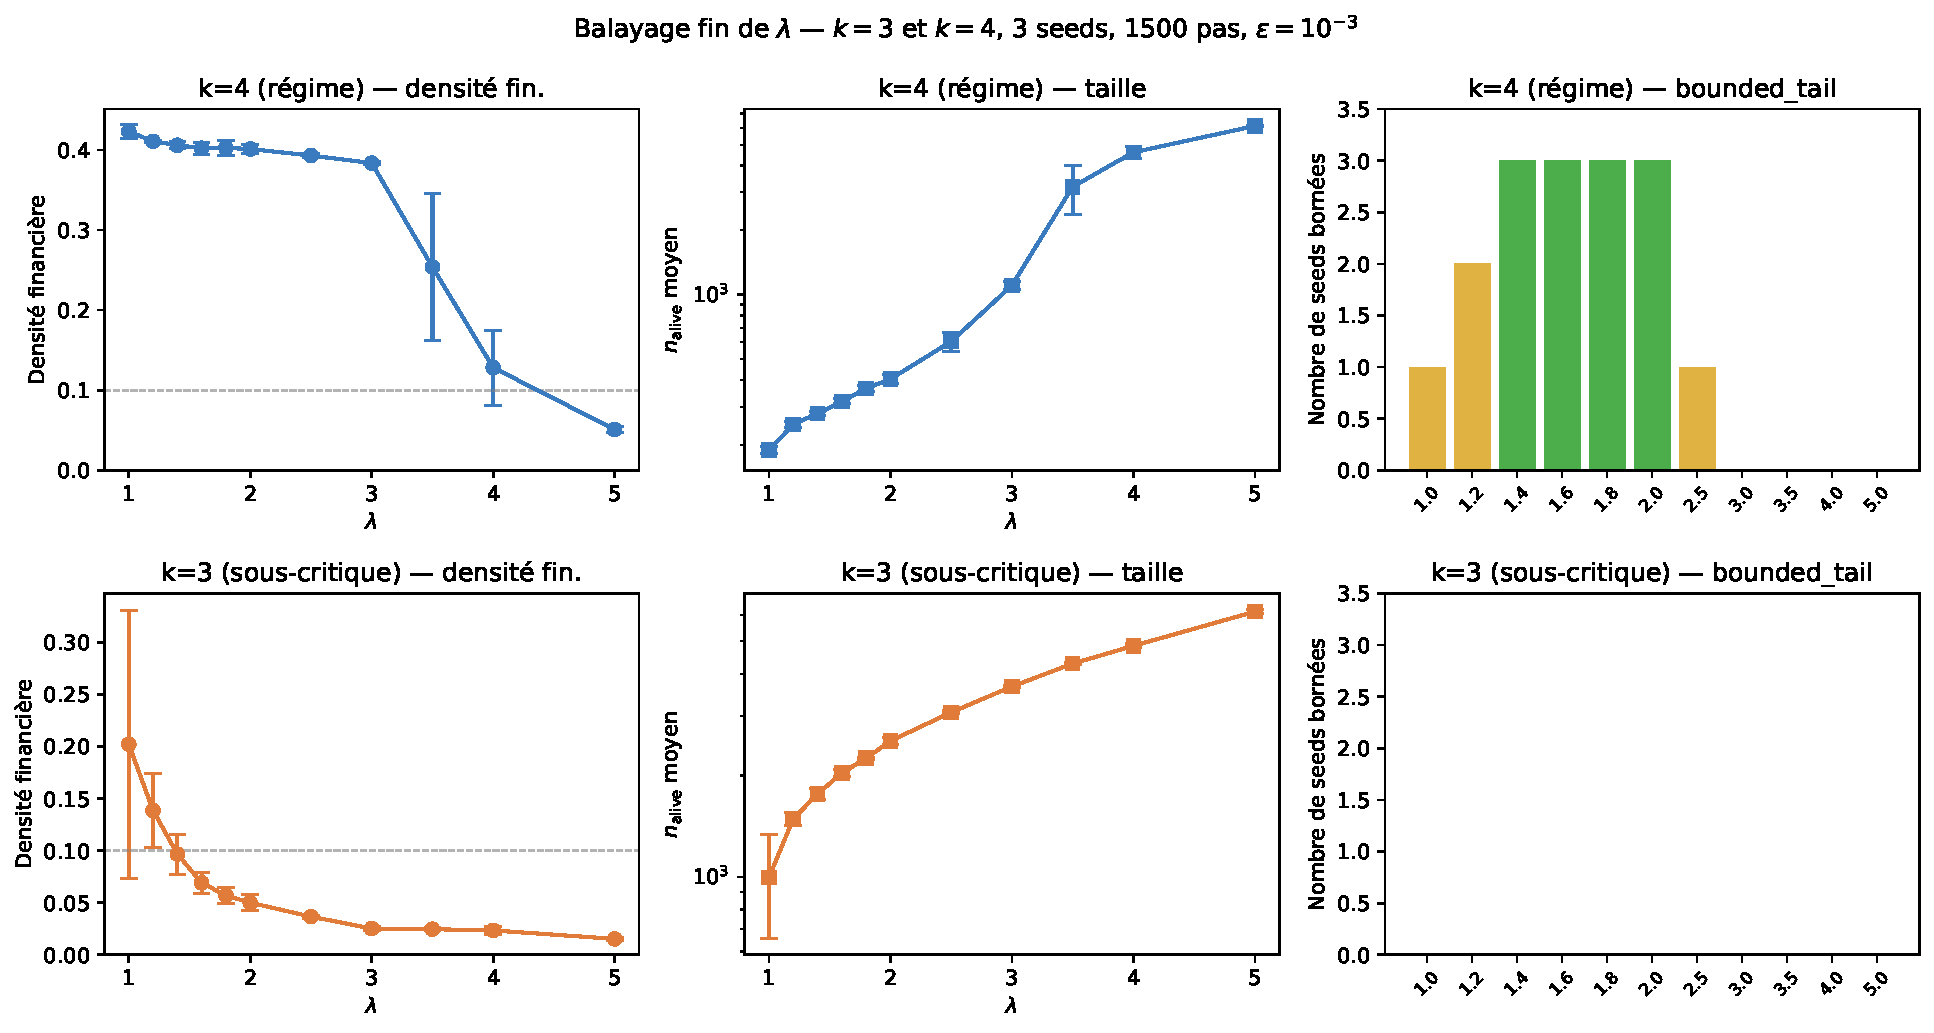
\includegraphics[width=0.98\linewidth]{figures/claude_lambda_fine_sweep.pdf}
  \caption{Balayage fin de \(\lambda\) pour \(k=4\) (bleu) et \(k=3\) (orange),
  $\epsilon=10^{-3}$, 1\,500 pas, 3 seeds (42, 7, 123).
  De gauche a droite :
  (1) densite financiere $d_f = V/A$ avec barres d'erreur inter-seeds ;
  (2) $n_{\mathrm{alive}}$ final en echelle log ;
  (3) nombre de seeds verifiant $\mathcal{B}$ (\texttt{bounded\_tail}).
  La frontiere de regime pour \(k=4\) se situe entre \(\lambda=2.0\)
  (3/3 bornes) et \(\lambda=2.5\) (1/3 bornee).}
\end{figure}

\section{Robustesse OAT : validation sur seeds 7 et 123}
\label{sec:oat-robustesse}

La campagne OAT initiale de Codex n'utilisait qu'un seul seed (42). Les 8
parametres les plus impactants ont ete revalides a seeds 7 et 123. Les ecarts-
types inter-seeds mesurent la robustesse de chaque effet.

\subsection*{Effets robustes sur le centre \(k=4\)}

\begin{table}[H]
\centering
\small
\begin{tabular}{lrrrr}
\toprule
Parametre (valeur) & $\mathcal{B}$/3s & $d_f$ (moy.$\pm$std) & note \\
\midrule
\(\alpha_\sigma=0.02\) & 3/3 & \(0.520\pm0.005\) & densification robuste \\
\(\mu=0.0\) & 3/3 & \(0.468\pm0.006\) & densification robuste \\
\(f=0.0\) (emprunteur) & 3/3 & \(0.453\pm0.001\) & densification robuste \\
actif initial 100 & 3/3 & \(0.446\pm0.007\) & densification robuste \\
\(\alpha_\sigma=0.005\) & 3/3 & \(0.443\pm0.003\) & densification robuste \\
\(\delta_{\mathrm{endo}}=0.02\) & 1/3 & \(0.457\pm0.003\) & \textbf{instable inter-seeds} \\
\(\theta=0.5\) & 1/3 & \(0.432\pm0.005\) & \textbf{instable inter-seeds} \\
\(\theta=0.2\) & 0/3 & \(0.040\pm0.004\) & destruction robuste \\
\(\mu=0.1\) & 0/3 & \(0.046\pm0.001\) & destruction robuste \\
\(\epsilon=10^{-2}\) & 0/3 & \(0.007\pm0.000\) & destruction robuste \\
\(f=0.5\) (emprunteur) & 0/3 & \(0.011\pm0.000\) & destruction robuste \\
actif initial 400 & 0/3 & \(0.031\pm0.004\) & destruction robuste \\
\(\delta_{\mathrm{endo}}=0.1\) & 0/3 & \(0.005\pm0.000\) & destruction robuste \\
\bottomrule
\end{tabular}
\caption{Robustesse OAT centre \(k=4\), 3 seeds. B.T.~3s = nombre de seeds a
queue bornee sur 3.}
\end{table}

Un resultat notable : \(\delta_{\mathrm{endo}}=0.02\) et \(\theta=0.5\)
etaient declares bornes sur seed=42 par Codex, mais ils ne passent le critere
que sur 1/3 seeds. Ces deux cas sont donc des \emph{effets vrais mais fragiles}
: la perturbation pousse le systeme vers la frontiere du regime plutot qu'au
centre. Ils ne doivent pas etre interpretes comme des effets robustes.

\subsection*{Effets robustes sur le centre \(k=3\)}

\begin{table}[H]
\centering
\small
\begin{tabular}{lrrrr}
\toprule
Parametre (valeur) & $\mathcal{B}$/3s & $d_f$ (moy.$\pm$std) & note \\
\midrule
\(\mu=0.0\) & 3/3 & \(0.479\pm0.002\) & entree robuste en regime \\
actif initial 100 & 2/3 & \(0.407\pm0.007\) & entree partielle en regime \\
\(\alpha_\sigma=0.02\) & 2/3 & \(0.489\pm0.008\) & entree partielle en regime \\
\(\delta_{\mathrm{endo}}=0.02\) & 2/3 & \(0.440\pm0.005\) & entree partielle en regime \\
\(\theta=0.5\) & 1/3 & \(0.230\pm0.074\) & tres dispersee, instable \\
\midrule
\(\theta=0.2\) & 0/3 & \(0.016\pm0.001\) & destruction robuste \\
\(\mu=0.1\) & 0/3 & \(0.021\pm0.000\) & destruction robuste \\
\(\epsilon=10^{-2}\) & 0/3 & \(0.004\pm0.000\) & destruction robuste \\
\(f=0.5\) (emprunteur) & 0/3 & \(0.007\pm0.000\) & destruction robuste \\
actif initial 400 & 0/3 & \(0.016\pm0.001\) & destruction robuste \\
\(\delta_{\mathrm{endo}}=0.1\) & 0/3 & \(0.003\pm0.000\) & destruction robuste \\
\bottomrule
\end{tabular}
\caption{Robustesse OAT centre \(k=3\), 3 seeds.}
\end{table}

\begin{figure}[H]
  \centering
  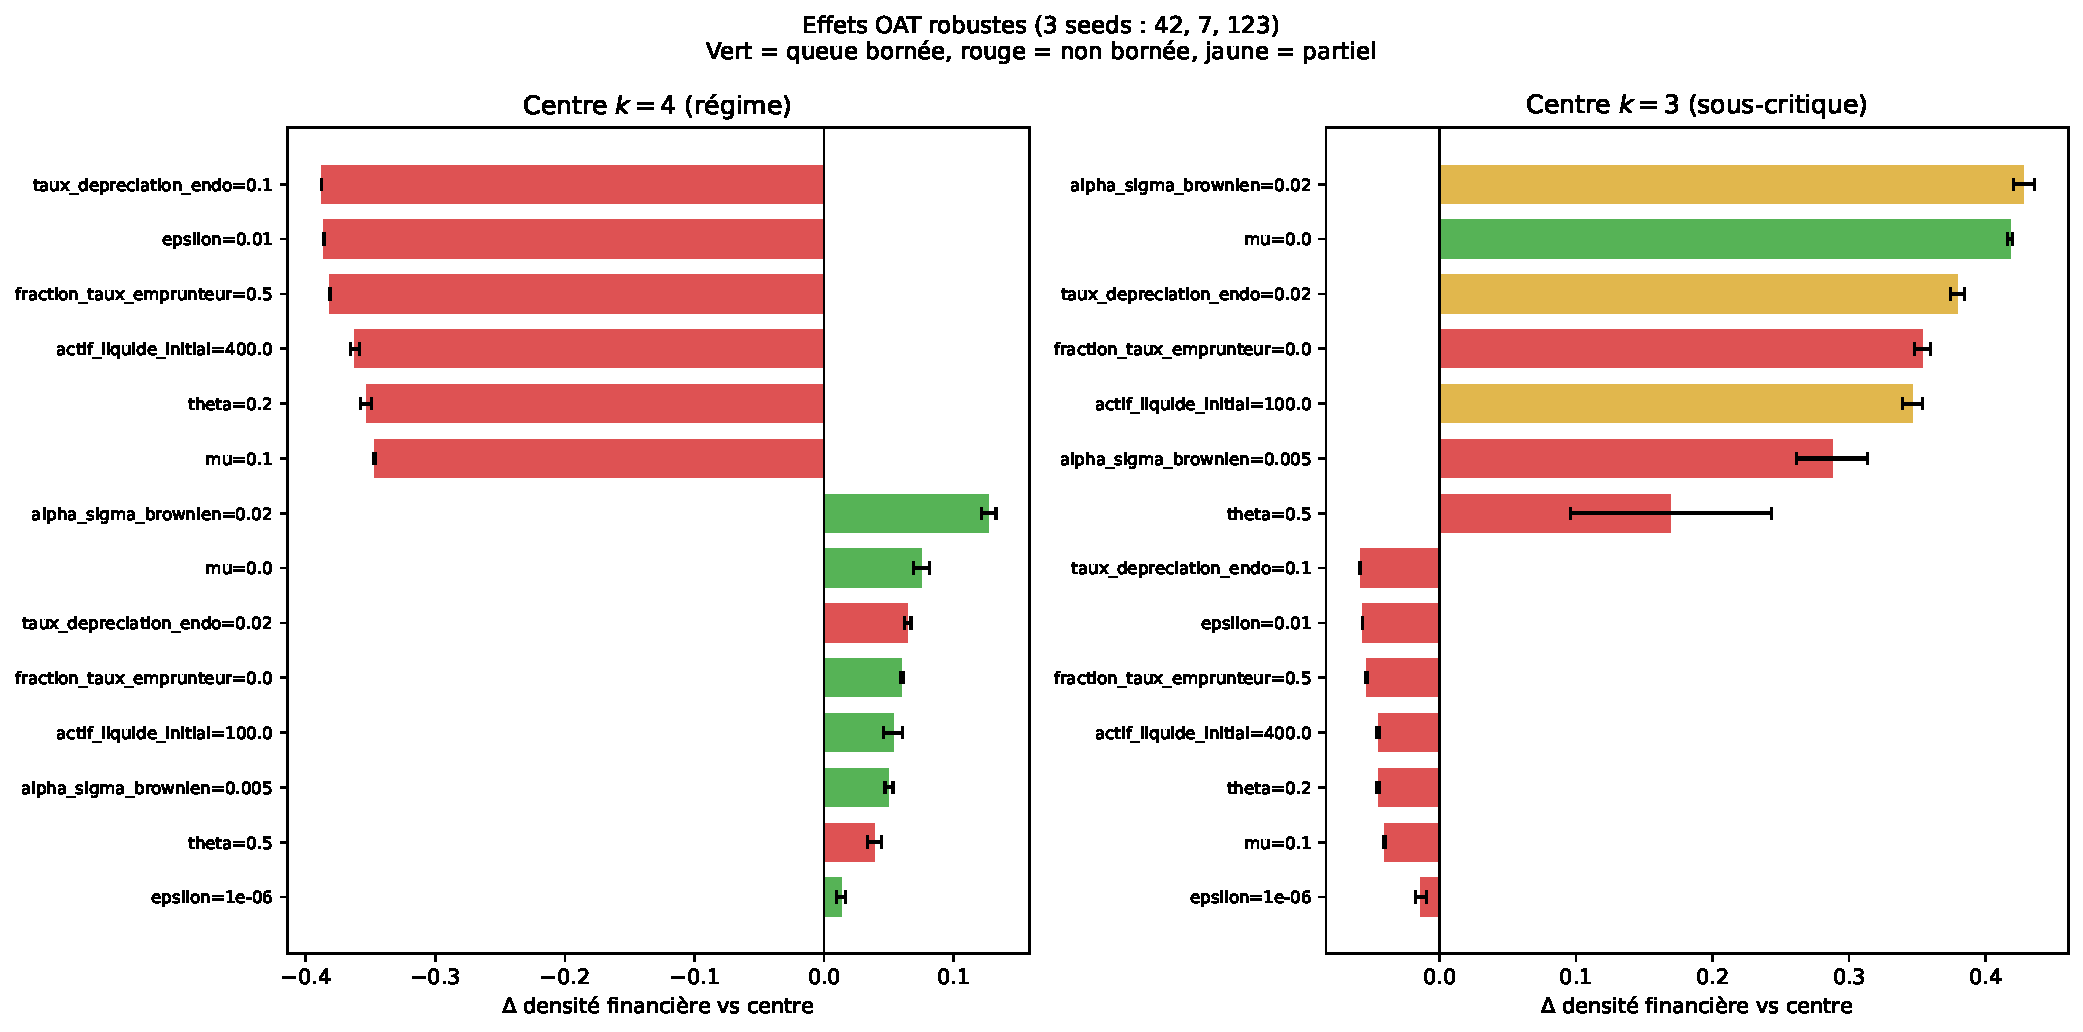
\includegraphics[width=0.98\linewidth]{figures/claude_oat_robustness.pdf}
  \caption{Effets OAT robustes (3 seeds). Les barres d'erreur representent
  l'ecart-type inter-seeds. Vert = queue bornee sur \(\ge 2/3\) seeds,
  rouge = bornee sur \(\le 1/3\), jaune = 1/3 ou 2/3.}
\end{figure}

\section{Cartes de phase : couplages systematiques}
\label{sec:couplages}

Quatre couplages a deux parametres ont ete simules (1500 pas, 3 seeds, grille
complete, \(\epsilon=10^{-3}\)), produisant chacun une carte de phase
\texttt{bounded\_share} moyennee sur les seeds.

\subsection*{Carte \(\lambda \times k\)}

\begin{table}[H]
\centering
\small
\begin{tabular}{rllllll}
\toprule
\(k\) \textbackslash{} \(\lambda\) & 1.0 & 1.5 & 2.0 & 2.5 & 3.0 & 4.0 \\
\midrule
2 & 0   & 0   & 0   & 0   & 0   & 0 \\
3 & 0   & 0   & 0   & 0   & 0   & 0 \\
4 & 0.3 & 0.3 & \textbf{1.0} & 0.3 & 0 & 0 \\
5 & 0   & 0.7 & 0.7 & \textbf{1.0} & \textbf{1.0} & \textbf{1.0} \\
6 & 0   & \textbf{1.0} & \textbf{1.0} & \textbf{1.0} & \textbf{1.0} & \textbf{1.0} \\
\bottomrule
\end{tabular}
\caption{Fraction de seeds a queue bornee, carte \(\lambda \times k\).
\(k \le 3\) ne forme jamais de regime en homogene (\(\sigma_\alpha=0\)).
La fenetre optimale de \(k=4\) est \(\lambda \approx 2.0\).}
\end{table}

\(k\) est le facteur dominant. L'augmentation de \(k\) abaisse le seuil
effectif en \(\lambda\) : a \(k=5\), le regime reste robuste jusqu'a
\(\lambda=4.0\), alors que \(k=4\) deja sorti du regime a cette valeur.

\begin{figure}[H]
  \centering
  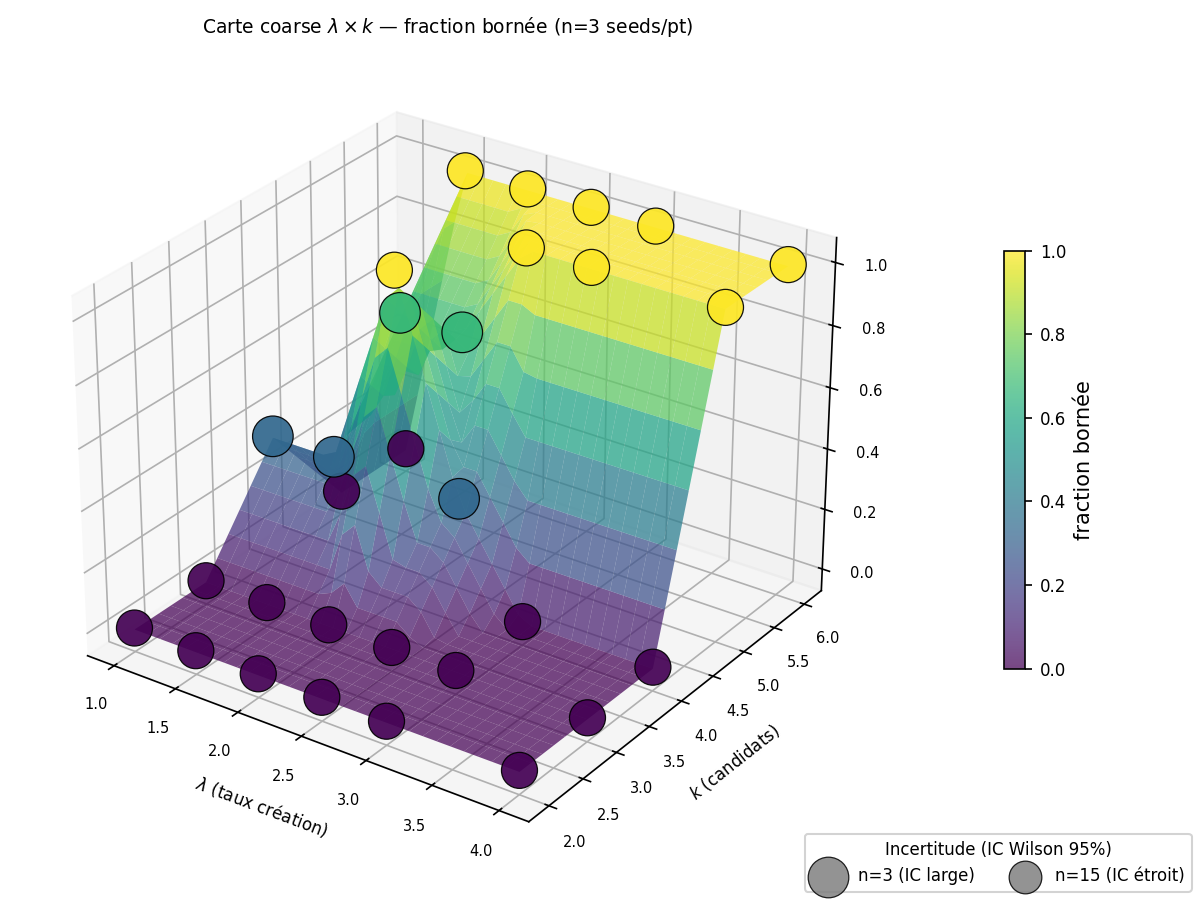
\includegraphics[width=0.80\linewidth]{figures/claude_surface_3d_lambda_k.png}
  \caption{Surface 3D de la carte coarse \(\lambda \times k\) : fraction de
  seeds a queue bornee (\(\mathcal{B}\)). Axe Z et couleur (viridis) : fraction
  $\in[0,1]$. Chaque point represente une cellule de grille (3 seeds).
  \(k \le 3\) ne forme jamais de regime en homogene (\(\sigma_\alpha=0\)).
  La fenetre optimale de \(k=4\) est \(\lambda\approx2.0\).}
\end{figure}

\subsection*{Carte \(k \times \mu\)}

\begin{table}[H]
\centering
\small
\begin{tabular}{rrrrrr}
\toprule
\(k\) \textbackslash{} \(\mu\) & 0.00 & 0.01 & 0.03 & 0.05 & 0.10 \\
\midrule
2 & \textbf{1.00} & 0    & 0    & 0    & 0 \\
3 & \textbf{1.00} & 0.67 & 0    & 0    & 0 \\
4 & \textbf{1.00} & 1.00 & 1.00 & 1.00 & 0 \\
5 & 0.67 & 1.00 & 1.00 & 0.67 & 0 \\
\bottomrule
\end{tabular}
\caption{Fraction de seeds a queue bornee, carte \(k \times \mu\).
\(\mu = \texttt{mu}\) est la prime de rendement minimal a l'emprunt.}
\end{table}

\textbf{Resultat majeur.} \(\mu=0\) debloque le regime meme pour \(k=2\)
et \(k=3\) (fraction 1.00). La valeur par defaut \(\mu=0.05\) empeche \(k \le 3\)
d'entrer en regime : c'est la prime minimale qui cree a elle seule le seuil de
phase pour les petits \(k\). Au dela de \(\mu=0.10\), aucun \(k\) ne forme de
regime borne. Ceci signifie que l'interpretation physique de \(k\) comme
\emph{seuil absolu} depend du choix de \(\mu\).

\begin{figure}[H]
  \centering
  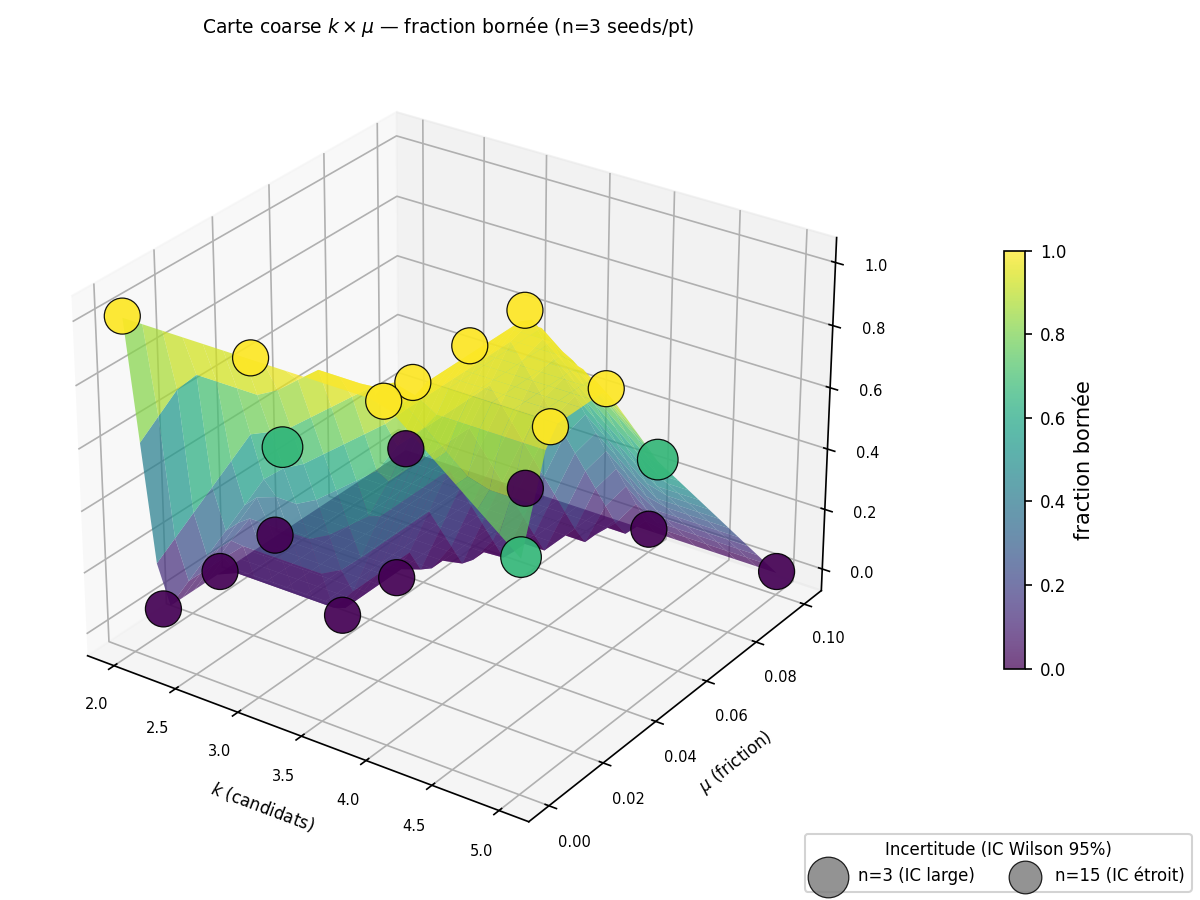
\includegraphics[width=0.80\linewidth]{figures/claude_surface_3d_k_mu.png}
  \caption{Surface 3D de la carte coarse \(k \times \mu\) : fraction de
  seeds a queue bornee (\(\mathcal{B}\)). Axe Z et couleur (viridis) : fraction
  $\in[0,1]$. Grille 4 valeurs de $k$ \(\times\) 5 valeurs de $\mu$, 3 seeds.
  Le role de porte de phase de \(\mu\) est visible :
  \(\mu > 0.10\) detruit tous les regimes.}
\end{figure}

\subsection*{Carte \(\sigma_\alpha \times k\)}

\begin{table}[H]
\centering
\small
\begin{tabular}{rrrrrr}
\toprule
\(k\) \textbackslash{} \(\sigma_\alpha\) & 0.000 & 0.003 & 0.010 & 0.020 & 0.050 \\
\midrule
2 & 0    & 0    & 0    & 0    & 0 \\
3 & 0    & 0    & 0.67 & 0.67 & 0 \\
4 & 1.00 & 1.00 & 0.67 & 1.00 & 0 \\
5 & 0.67 & 0.67 & 0.33 & 1.00 & 0 \\
\bottomrule
\end{tabular}
\caption{Fraction de seeds a queue bornee, carte \(\sigma_\alpha \times k\).}
\end{table}

La volatilite \(\sigma_\alpha\) ouvre une fenetre de regime pour \(k=3\)
autour de \([0.01, 0.02]\), confirmant le balayage precedent. A
\(\sigma_\alpha=0.05\), tous les regimes disparaissent quelle que soit \(k\) :
la volatilite excessive fragmente le reseau.

\begin{figure}[H]
  \centering
  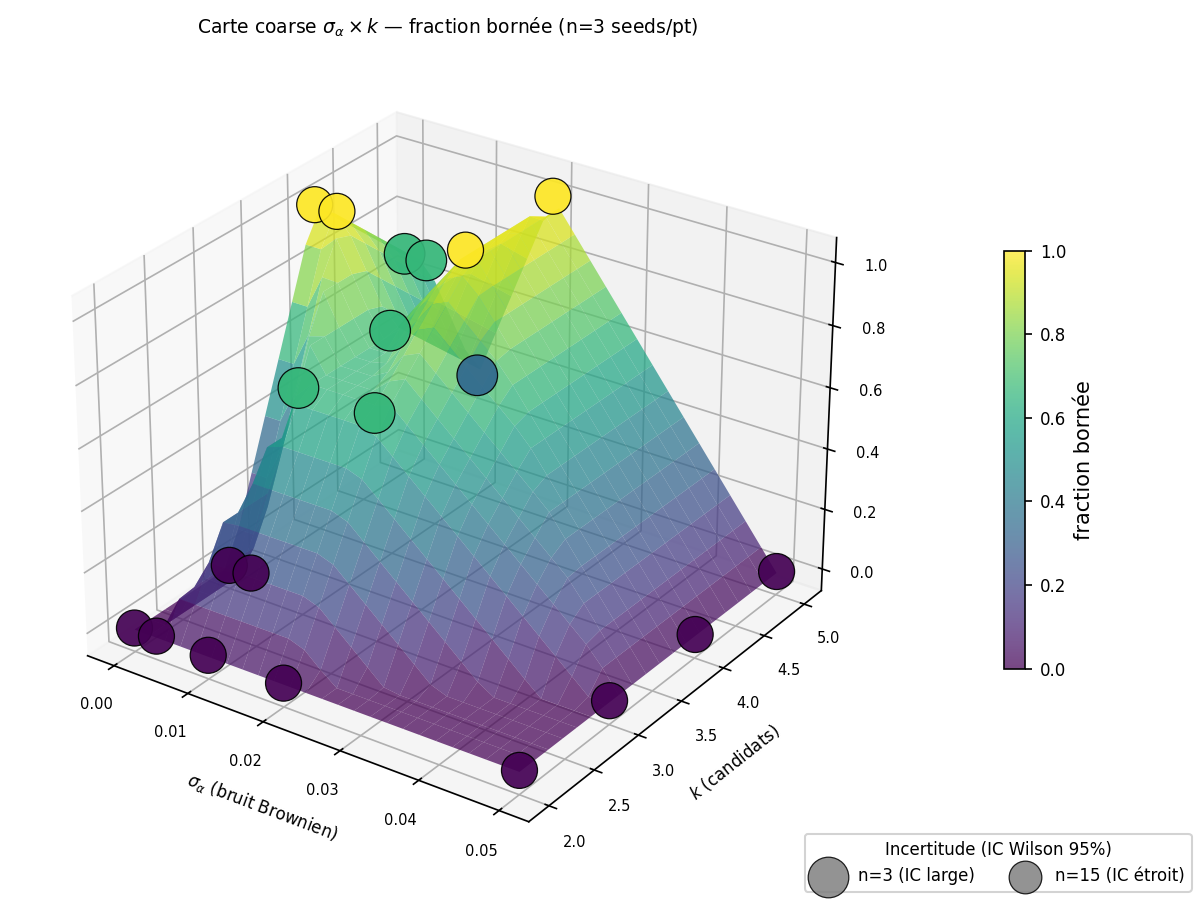
\includegraphics[width=0.80\linewidth]{figures/claude_surface_3d_sigma_k.png}
  \caption{Surface 3D de la carte coarse \(\sigma_\alpha \times k\) : fraction
  de seeds a queue bornee (\(\mathcal{B}\)). Axe Z et couleur (viridis) :
  fraction $\in[0,1]$. Grille 5 valeurs de $\sigma_\alpha$
  $\times$ 4 valeurs de $k$, 3 seeds.
  La fenetre active $\sigma_\alpha\in[0.01, 0.02]$ pour $k=3$ est etroite ;
  $\sigma_\alpha=0.05$ est destructeur universel.}
\end{figure}

\subsection*{Carte \(\theta \times \delta_{\mathrm{endo}}\)}

\begin{table}[H]
\centering
\small
\begin{tabular}{rrrr}
\toprule
\(\theta\) \textbackslash{} \(\delta_{\mathrm{endo}}\) & 0.02 & 0.05 & 0.10 \\
\midrule
\multicolumn{4}{l}{\emph{Centre \(k=3\)}} \\
0.20 & 0.7 & 0.0 & 0.0 \\
0.35 & 0.7 & 0.0 & 0.0 \\
0.50 & 0.7 & 0.3 & 0.0 \\
\midrule
\multicolumn{4}{l}{\emph{Centre \(k=4\)}} \\
0.20 & 0.7 & 0.0 & 0.0 \\
0.35 & 0.3 & 1.0 & 0.0 \\
0.50 & 0.3 & 0.3 & 0.0 \\
\bottomrule
\end{tabular}
\caption{Fraction de seeds a queue bornee, carte \(\theta \times
\delta_{\mathrm{endo}}\), lignes selectives (table abregee).
\(\theta\) est la part du gain extraite,
\(\delta_{\mathrm{endo}}\) le taux de depreciation endogene.}
\end{table}

\(\delta_{\mathrm{endo}}=0.10\) detruit systematiquement le regime pour
tout \(\theta\) et tout \(k\). A \(\delta_{\mathrm{endo}}=0.02\),
les resultats sont stochastiques : le systeme se trouve pres de la frontiere.
Pour \(k=4\), \(\delta_{\mathrm{endo}}=0.05\) avec \(\theta=0.35\) donne
paradoxalement 1.00, ce qui suggere une interaction non monotone entre
extraction et depreciation.

\begin{figure}[H]
  \centering
  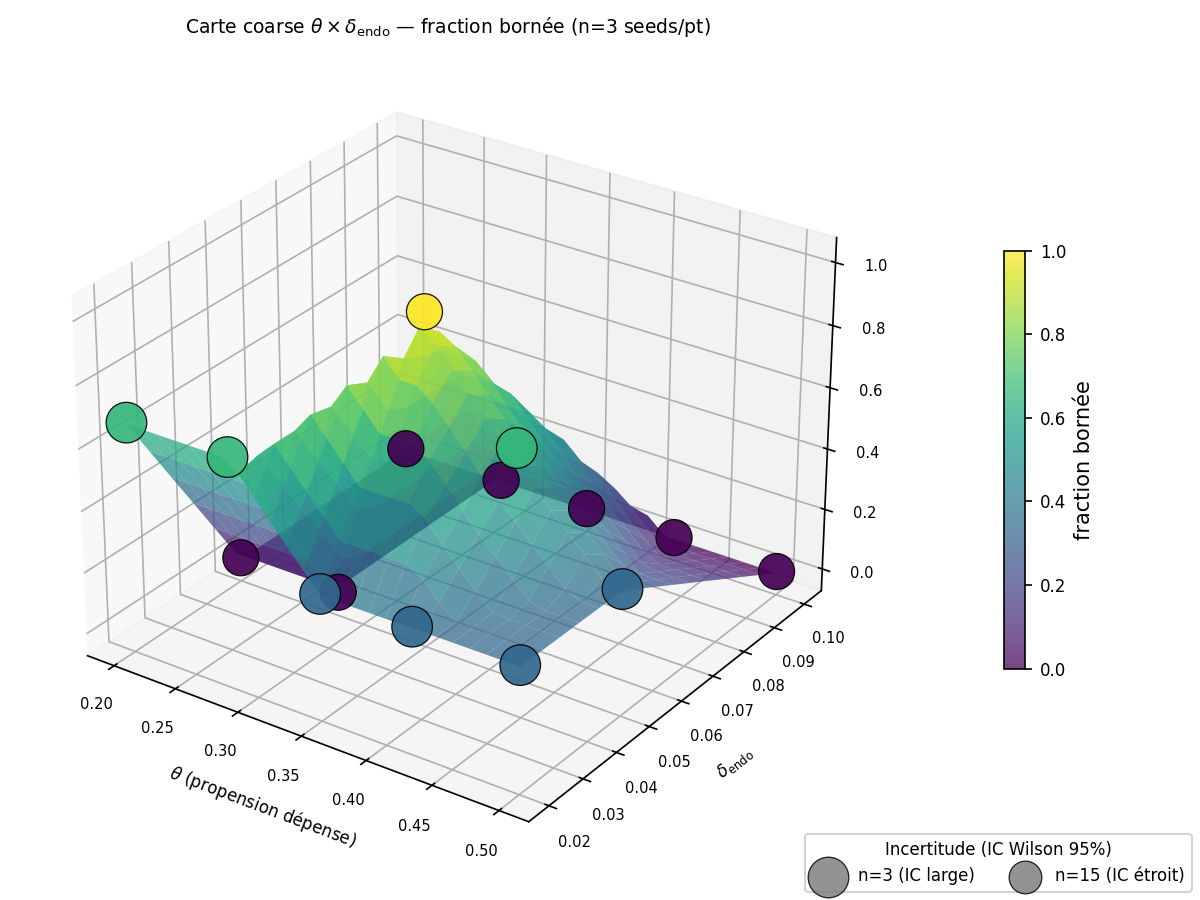
\includegraphics[width=0.80\linewidth]{figures/claude_surface_3d_theta_delta.png}
  \caption{Surface 3D de la carte coarse \(\theta \times \delta_{\mathrm{endo}}\) :
  fraction de seeds a queue bornee (\(\mathcal{B}\)). Axe Z et couleur (viridis) :
  fraction $\in[0,1]$. Grille 3 valeurs de $\theta$
  $\times$ 3 valeurs de $\delta_{\mathrm{endo}}$, 3 seeds, deux centres
  ($k=3$ et $k=4$).
  \(\delta_{\mathrm{endo}}=0.10\) detruit systematiquement le regime.}
\end{figure}

\section{Campagnes adaptatives : cartes de phase denses}
\label{sec:campagnes-adaptatives}

Les cartes de phase de la section precedente reposaient sur des grilles grossieres
(3--6 valeurs par axe, 3 seeds). Quatre campagnes a echantillonnage adaptatif
ont ete ensuite conduites pour densifier ces cartes.
Le protocole adaptatif alloue 3 seeds dans les zones stables, jusqu'a 15 seeds
sur les frontieres detectees (\(0.1 < \mathcal{B}\text{-rate} < 0.9\)).
Les fractions presentees dans les tables ci-dessous sont la fraction de seeds
verifiant \(\mathcal{B}\) (\texttt{bounded\_tail = True}), notees sous
la forme \textbf{bornes/total} (ex. : 7/15). Le critere de stationnarite
dual --- \(\mathcal{B} \wedge |r_f - 1| < 0.15\) --- est utilise pour
la classification interne des cellules mais n'est pas repris dans les tables.
Les parametres de depreciation sont \emph{unifies} (\(\delta_{\mathrm{endo}} = \delta_{\mathrm{exo}} = \delta_{\mathrm{liquide}} = \delta\))
dans la campagne \(\theta \times \delta\), supprimant un degre de liberte
parasite de la campagne coarse.
\smallskip

\noindent\textit{Note sur l'incertitude :}
$n=3$ dans les zones stables (fraction 0 ou 1 confirmee) ;
$n=15$ aux frontieres detectees ($0 < \mathcal{B}\text{-rate} < 1$).
Pour $n=3$, l'IC Wilson 95\,\% d'une fraction $2/3$ est $[0.19, 0.93]$ ;
pour $n=15$ avec $10/15$, il est $[0.46, 0.87]$. Ne pas sur-interpreter
les fractions intermediaires a $n=3$.

\paragraph{Volume total.}
1\,479 runs au total (417 + 327 + 267 + 468), executes entre avril et mai 2026.

\subsection*{Campagne \(\lambda \times k\) etendue (417 runs)}

\begin{table}[H]
\centering
\footnotesize
\begin{tabular}{r|rrrrrrr}
\toprule
\(\lambda \backslash k\) & 2 & 3 & 4 & 5 & 6 & 7 & 8 \\
\midrule
0.5 & 2/15 & 6/15 & 9/15 & 0/3 & 0/3 & 1/15 & 0/3 \\
1.0 & 0/3 & 0/3 & \textbf{3/3} & 10/15 & 0/3 & 0/3 & 6/15 \\
1.5 & 0/3 & 7/15 & 13/15 & 12/15 & 4/15 & 0/3 & 0/3 \\
2.0 & 0/3 & 0/3 & 13/15 & \textbf{3/3} & 6/15 & 4/15 & 0/3 \\
2.5 & 0/3 & 0/3 & \textbf{3/3} & \textbf{3/3} & 11/15 & 6/15 & \textbf{3/3} \\
3.0 & 0/3 & 0/3 & \textbf{3/3} & \textbf{3/3} & \textbf{3/3} & 11/15 & \textbf{3/3} \\
4.0 & 0/3 & 0/3 & 11/15 & \textbf{3/3} & \textbf{3/3} & \textbf{3/3} & 12/15 \\
5.0 & 0/3 & 0/3 & 8/15 & \textbf{3/3} & \textbf{3/3} & \textbf{3/3} & \textbf{3/3} \\
6.0 & 0/3 & 0/3 & 0/3 & \textbf{3/3} & \textbf{3/3} & \textbf{3/3} & \textbf{3/3} \\
\bottomrule
\end{tabular}
\caption{Seeds bornes / total par cellule (\(\mathcal{B}\) = \texttt{bounded\_tail}),
carte \(\lambda \times k\) adaptative (417 runs, grille fine).
\textbf{Gras} = fraction \(\ge 0.9\).
$n=3$ dans les zones stables (fraction 0 ou 1), $n=15$ aux frontieres.
\(\lambda = \texttt{lambda\_creation}\), \(k = \texttt{n\_candidats\_pool}\).}
\end{table}

\begin{figure}[H]
  \centering
  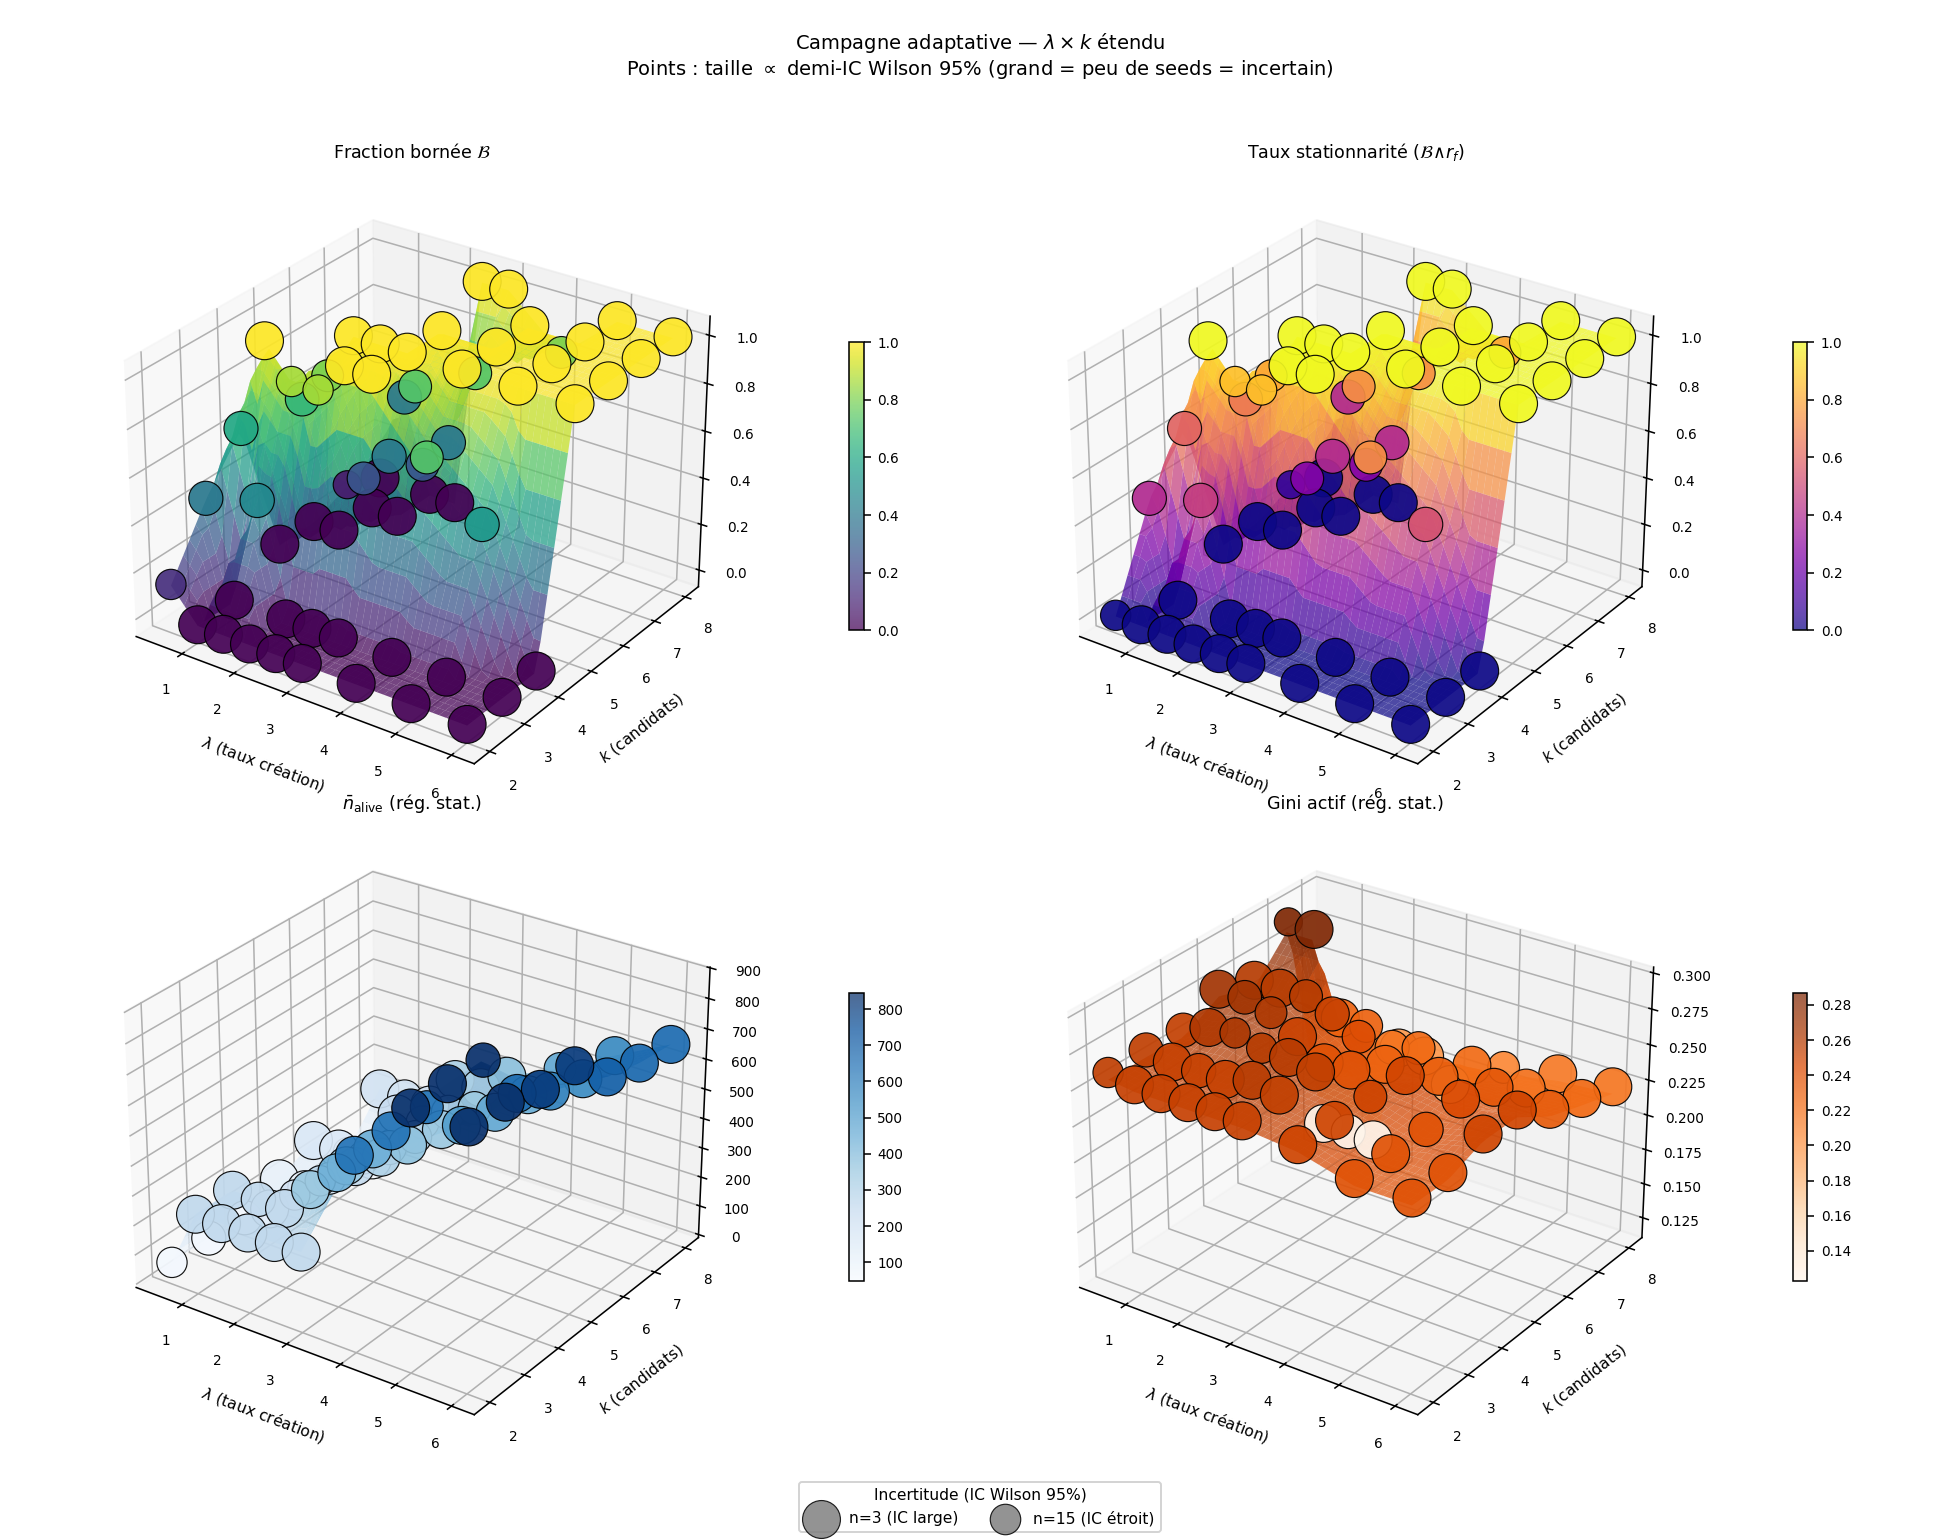
\includegraphics[width=\linewidth]{figures/map_lambda_k_3d.png}
  \caption{Cartes 3D adaptatives \(\lambda \times k\) (417 runs, 1500 pas) en
  disposition 2\(\times\)2 : fraction bornee \(\mathcal{B}\) (haut-gauche),
  taux stationnarite \(\mathcal{B}\wedge r_f\) (haut-droit),
  \(\bar{n}_{\mathrm{alive}}\) en regime (bas-gauche),
  Gini actif (bas-droit).
  Surface interpolee (scipy linaire) sur grille \(9\times 7\).
  Points superposes : couleur = valeur locale, \textbf{taille} $\propto$
  demi-IC Wilson 95\% (grand = incertain, i.e.\ $n=3$ seeds~; petit = $n=15$).
  Le seuil \(k\ge 4\) et la zone robuste \(\lambda \in [1.5, 3.0]\) sont confirmes.}
\end{figure}

\textbf{Resultats robustes.}
Le seuil \(k=4\) comme minimum de regime est confirme : \(k \le 3\) donne toujours
0 sauf \(\lambda=0.5\) ou \(k=3\) (\(0.47\)) et \(\lambda=1.5\).
Au-dela de \(k \ge 5\), le regime est robuste sur une plage etendue de \(\lambda\)
(jusqu'a \(\lambda=5.0\) a \(k=5, 6, 7, 8\)).
La densite financiere dans les runs converges est stable :
\(\bar{d}_f = 0.236 \pm 0.023\), confirmant son role de \emph{parametre de reponse}
peu sensible a \((\lambda, k)\) dans la zone de regime.
Le nombre de prets par entite est lui aussi remarquablement stable : $\approx 10.4 \pm 1.8$.
En revanche, $n_{\mathrm{alive}}$ est tres variable dans la zone convergee
(61 a 913), signalant que la taille demographique depend fortement de \(\lambda\).

\subsection*{Campagne \(k \times \mu\) etendue (327 runs)}

\begin{table}[H]
\centering
\footnotesize
\begin{tabular}{r|rrrrrrrrr}
\toprule
\(k \backslash \mu\) & 0.00 & 0.01 & 0.02 & 0.03 & 0.05 & 0.07 & 0.10 & 0.13 & 0.15 \\
\midrule
2 & 10/15 & 4/15 & 0/3 & 0/3 & 0/3 & 0/3 & 0/3 & 0/3 & 0/3 \\
3 & 8/15 & 0/3 & 7/15 & 6/15 & 0/3 & 0/3 & 0/3 & 0/3 & 0/3 \\
4 & \textbf{3/3} & \textbf{3/3} & 12/15 & \textbf{3/3} & 13/15 & 7/15 & 0/3 & 0/3 & 0/3 \\
5 & \textbf{3/3} & 8/15 & 8/15 & 12/15 & \textbf{3/3} & \textbf{3/3} & 8/15 & 0/3 & 0/3 \\
6 & 11/15 & \textbf{3/3} & 7/15 & 3/15 & 6/15 & \textbf{3/3} & \textbf{3/3} & 0/3 & 0/3 \\
\bottomrule
\end{tabular}
\caption{Seeds bornes / total par cellule (\(\mathcal{B}\)), carte
\(k \times \mu\) adaptative (327 runs).
\textbf{Gras} = fraction \(\ge 0.9\).
$n=3$ dans les zones stables, $n=15$ aux frontieres.
\(\mu = \texttt{mu}\) : prime minimale au rendement de l'emprunt.}
\end{table}

\begin{figure}[H]
  \centering
  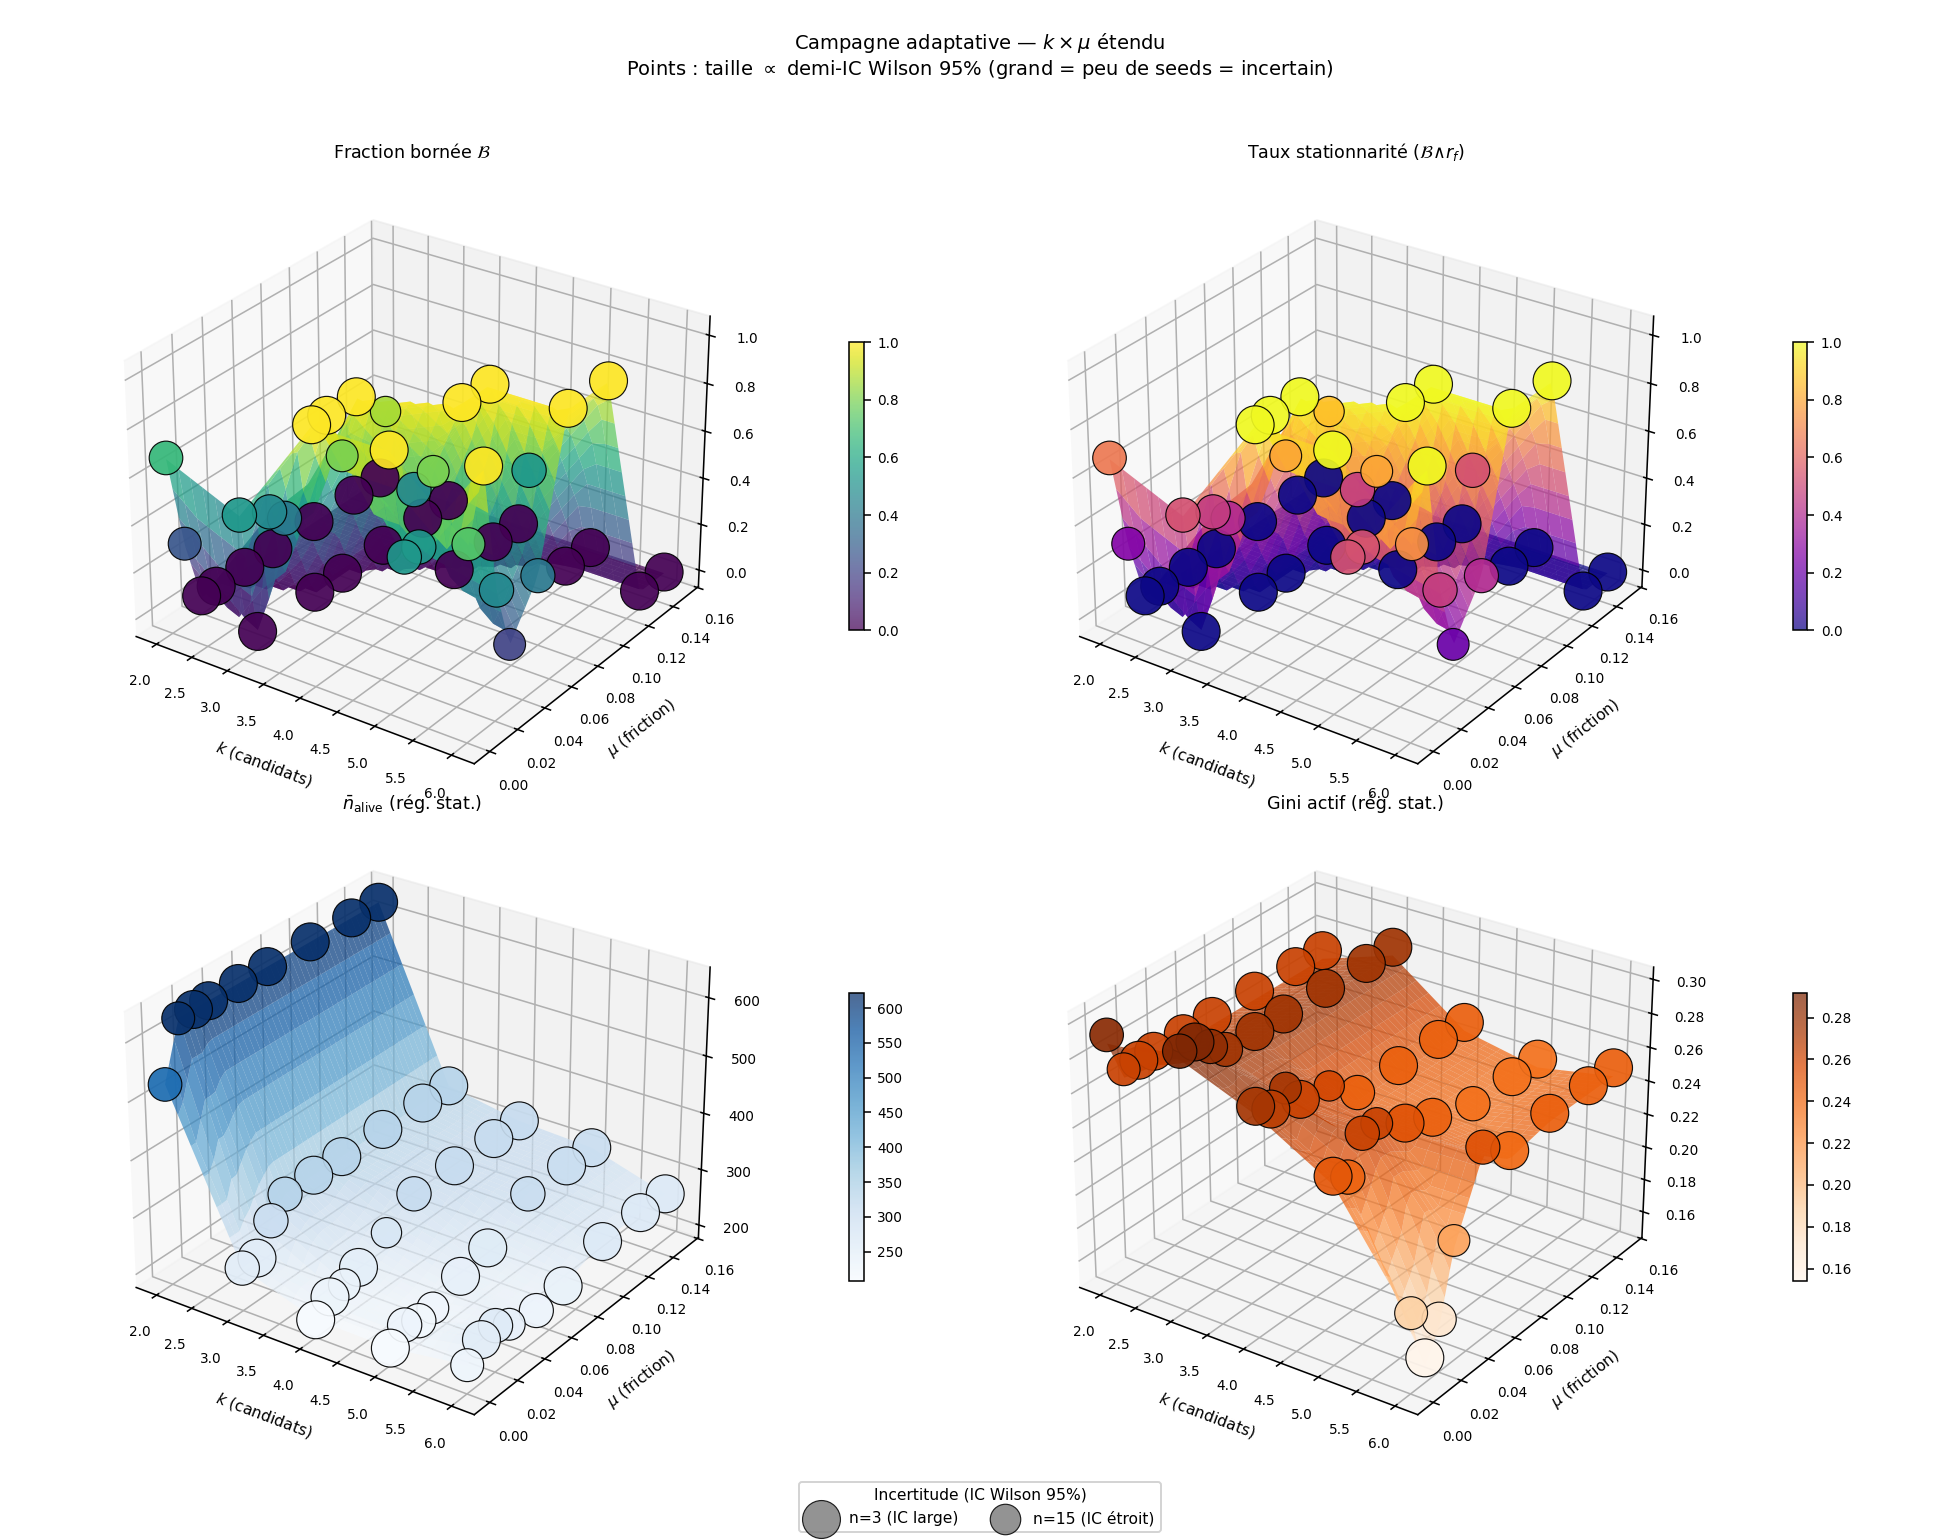
\includegraphics[width=\linewidth]{figures/map_k_mu_3d.png}
  \caption{Cartes 3D adaptatives \(k \times \mu\) (327 runs, 1500 pas) en
  disposition 2\(\times\)2.
  Axes \(k\) et \(\mu\) inverses (origine au coin arriere) pour degager la zone
  de regime actif. Points superposes : taille $\propto$ demi-IC Wilson 95\%
  (grand = $n=3$, incertain ; petit = $n=15$, robuste).
  La porte de phase \(\mu > 0.10\) est visible sur toutes les vues.}
\end{figure}

\textbf{Resultats robustes.}
\(\mu\) agit comme une \emph{porte de phase} independante : au-dela de \(\mu = 0.10\),
aucun \(k\) ne produit de regime borne.
\(\mu = 0\) debloque \(k=2\) (0.67) et \(k=3\) (0.53), montrant que le seuil
apparent \(k=4\) de la campagne coarse est artefacte par le choix \(\mu=0.05\).
La densite financiere dans les runs converges est tres stable :
\(\bar{d}_f = 0.243 \pm 0.022\), range \([0.195, 0.288]\).
Le taux de faillite est egalement tres stable : \(2.06 \pm 0.09\),
suggerant que le regime borne a une \emph{structure interne robuste}
independamment de \((k, \mu)\) dans sa zone d'existence.

\textbf{Mise en garde.} Les cartes \(k \times \mu\) montrent des zones de
non-monotonie marquee (par exemple \(k=3\) : fraction 0.53 a \(\mu=0\), 0.00
a \(\mu=0.01\), 0.47 a \(\mu=0.02\)). Ces fluctuations refleteront soit des
effets de front de phase, soit des artefacts du petit nombre de seeds aux
frontieres. Elles ne doivent pas etre interpretees comme des resonances.

\subsection*{Campagne \(\sigma_\alpha \times k\) etendue (267 runs)}

\begin{table}[H]
\centering
\footnotesize
\begin{tabular}{r|rrrrr}
\toprule
\(\sigma_\alpha \backslash k\) & 2 & 3 & 4 & 5 & 6 \\
\midrule
0.000 & 0/3 & 0/3 & 13/15 & \textbf{3/3} & 6/15 \\
0.003 & 0/3 & 0/3 & \textbf{3/3} & \textbf{3/3} & \textbf{3/3} \\
0.007 & 0/3 & 0/3 & 8/15 & 9/15 & \textbf{3/3} \\
0.010 & 0/3 & 4/15 & 5/15 & 12/15 & \textbf{3/3} \\
0.020 & 0/3 & 2/15 & 2/15 & 5/15 & 7/15 \\
0.035 & 0/3 & 0/3 & 0/3 & 0/3 & 0/3 \\
0.050 & 0/3 & 0/3 & 0/3 & 0/3 & 0/3 \\
0.075 & 0/3 & 0/3 & 0/3 & 0/3 & 0/3 \\
0.100 & 0/3 & 0/3 & 0/3 & 0/3 & 0/3 \\
\bottomrule
\end{tabular}
\caption{Seeds bornes / total par cellule (\(\mathcal{B}\)), carte
\(\sigma_\alpha \times k\) adaptative (267 runs).
\textbf{Gras} = fraction \(\ge 0.9\).
$n=3$ dans les zones stables, $n=15$ aux frontieres.
La destruction universelle a \(\sigma_\alpha \ge 0.035\) est confirmee pour
toutes les valeurs de \(k\) testees.
\(\sigma_\alpha = \texttt{alpha\_sigma\_brownien}\).}
\end{table}

\begin{figure}[H]
  \centering
  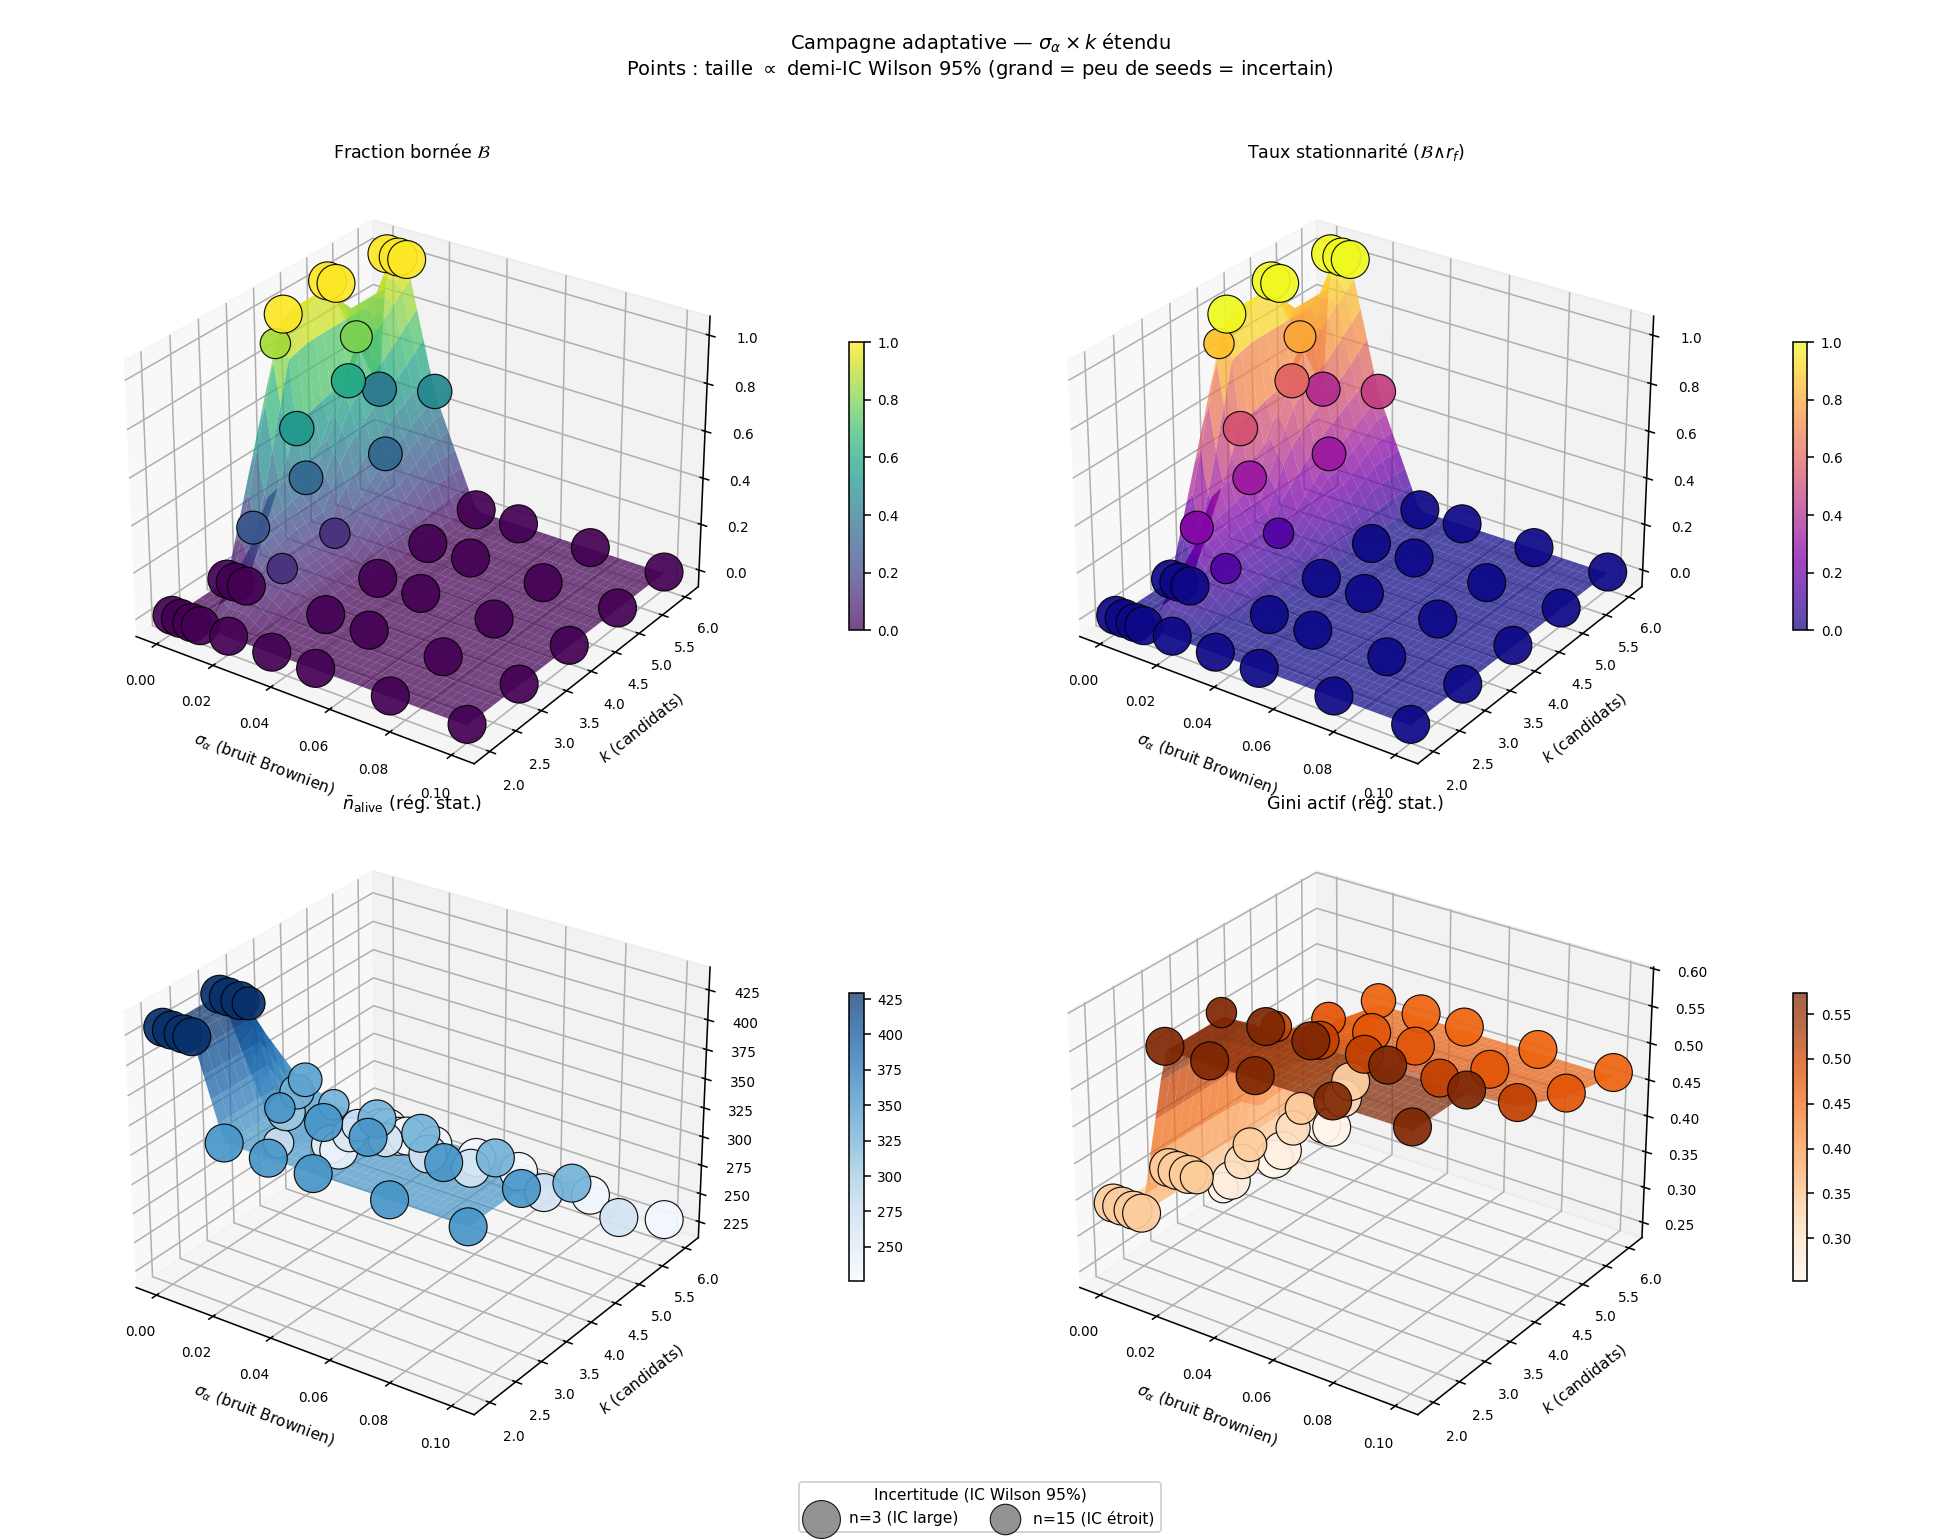
\includegraphics[width=\linewidth]{figures/map_sigma_k_3d.png}
  \caption{Cartes 3D adaptatives \(\sigma_\alpha \times k\) (267 runs, 1500 pas) en
  disposition 2\(\times\)2.
  Points superposes : taille $\propto$ demi-IC Wilson 95\%.
  La coupure nette a \(\sigma_\alpha = 0.035\) (seuil destructeur universel) est
  visible sur les quatre vues. \(k=6\) est le plus resilient au bruit Brownien.}
\end{figure}

\textbf{Resultats robustes.}
Le seuil \(\sigma_\alpha = 0.035\) est un \emph{destructeur universel} :
aucun run n'est borne au-dessus, pour tout \(k\) teste.
La fenetre de regime pour \(k=3\) est etroite et fragile : fraction 0.13--0.27
autour de \(\sigma_\alpha = 0.01\)--\(0.02\), soit tres sensible au seed.
\(k=6\) est le plus resilient : fraction 1.00 pour \(\sigma_\alpha \in [0.003, 0.010]\).
La densite financiere dans les runs converges est legere-ment plus elevee qu'en
regime statique : \(\bar{d}_f = 0.272 \pm 0.034\), et la concentration en actif
(Gini) est plus forte : \(\bar{G} = 0.31\), suggerant que la volatilite du rendement
produit une \emph{stratification} plus marquee des bilans.
Ce resultat est plausible mais fragile sur les 91 runs converges disponibles.

\subsection*{Campagne \(\theta \times \delta\) unifiee (468 runs)}

\paragraph{Contrainte de la campagne.}
Dans cette campagne, \(\delta_{\mathrm{endo}} = \delta_{\mathrm{exo}} = \delta_{\mathrm{liquide}} = \delta\)
(depreciation unifiee). Les deux degres de liberte parasites de la campagne
coarse sont supprimes.

\begin{table}[H]
\centering
\footnotesize
\begin{tabular}{r|rrrrrrrr}
\toprule
\(\theta \backslash \delta\) & 0.01 & 0.02 & 0.03 & 0.05 & 0.07 & 0.10 & 0.12$^\dagger$ & 0.15$^\dagger$ \\
\midrule
0.15 & 0/3 & 10/15 & 10/15 & 0/3 & 0/3 & 0/3 & \textbf{3/3} & \textbf{3/3} \\
0.20 & 0/3 & 0/3 & 10/15 & 0/3 & 0/3 & 0/3 & \textbf{3/3} & \textbf{3/3} \\
0.25 & 0/3 & 8/15 & 9/15 & 0/3 & 0/3 & 0/3 & \textbf{3/3} & \textbf{3/3} \\
0.28 & 0/3 & 11/15 & 6/15 & 0/3 & 0/3 & 0/3 & \textbf{3/3} & \textbf{3/3} \\
0.32 & 0/3 & 10/15 & 7/15 & 0/3 & 0/3 & 0/3 & \textbf{3/3} & \textbf{3/3} \\
0.35 & 0/3 & \textbf{3/3} & 4/15 & 0/3 & 0/3 & 0/3 & \textbf{3/3} & \textbf{3/3} \\
0.40 & 0/3 & \textbf{3/3} & 6/15 & 10/15 & 0/3 & 0/3 & \textbf{3/3} & \textbf{3/3} \\
0.45 & 0/3 & 10/15 & 4/15 & 6/15 & 0/3 & 0/3 & \textbf{3/3} & \textbf{3/3} \\
0.50 & 0/3 & 13/15 & 4/15 & 0/3 & 0/3 & 0/3 & \textbf{3/3} & \textbf{3/3} \\
0.55 & 0/3 & \textbf{3/3} & 5/15 & 1/15 & 0/3 & 0/3 & \textbf{3/3} & \textbf{3/3} \\
\bottomrule
\end{tabular}
\caption{Seeds bornes / total par cellule (\(\mathcal{B}\)), carte
\(\theta \times \delta\) unifiee (468 runs).
\textbf{Gras} = fraction \(\ge 0.9\).
$n=3$ dans les zones stables, $n=15$ aux frontieres.
$\dagger$ = colonnes d'extinction (\(n_{\mathrm{alive}} \approx 0\), artefact --
ne pas interpreter comme regime actif ; voir texte).
\(\theta = \texttt{theta}\) : part du gain extraite ;
\(\delta = \texttt{taux\_depreciation\_endo} = \texttt{taux\_depreciation\_exo}\)
(unifie dans cette campagne).}
\end{table}

\begin{figure}[H]
  \centering
  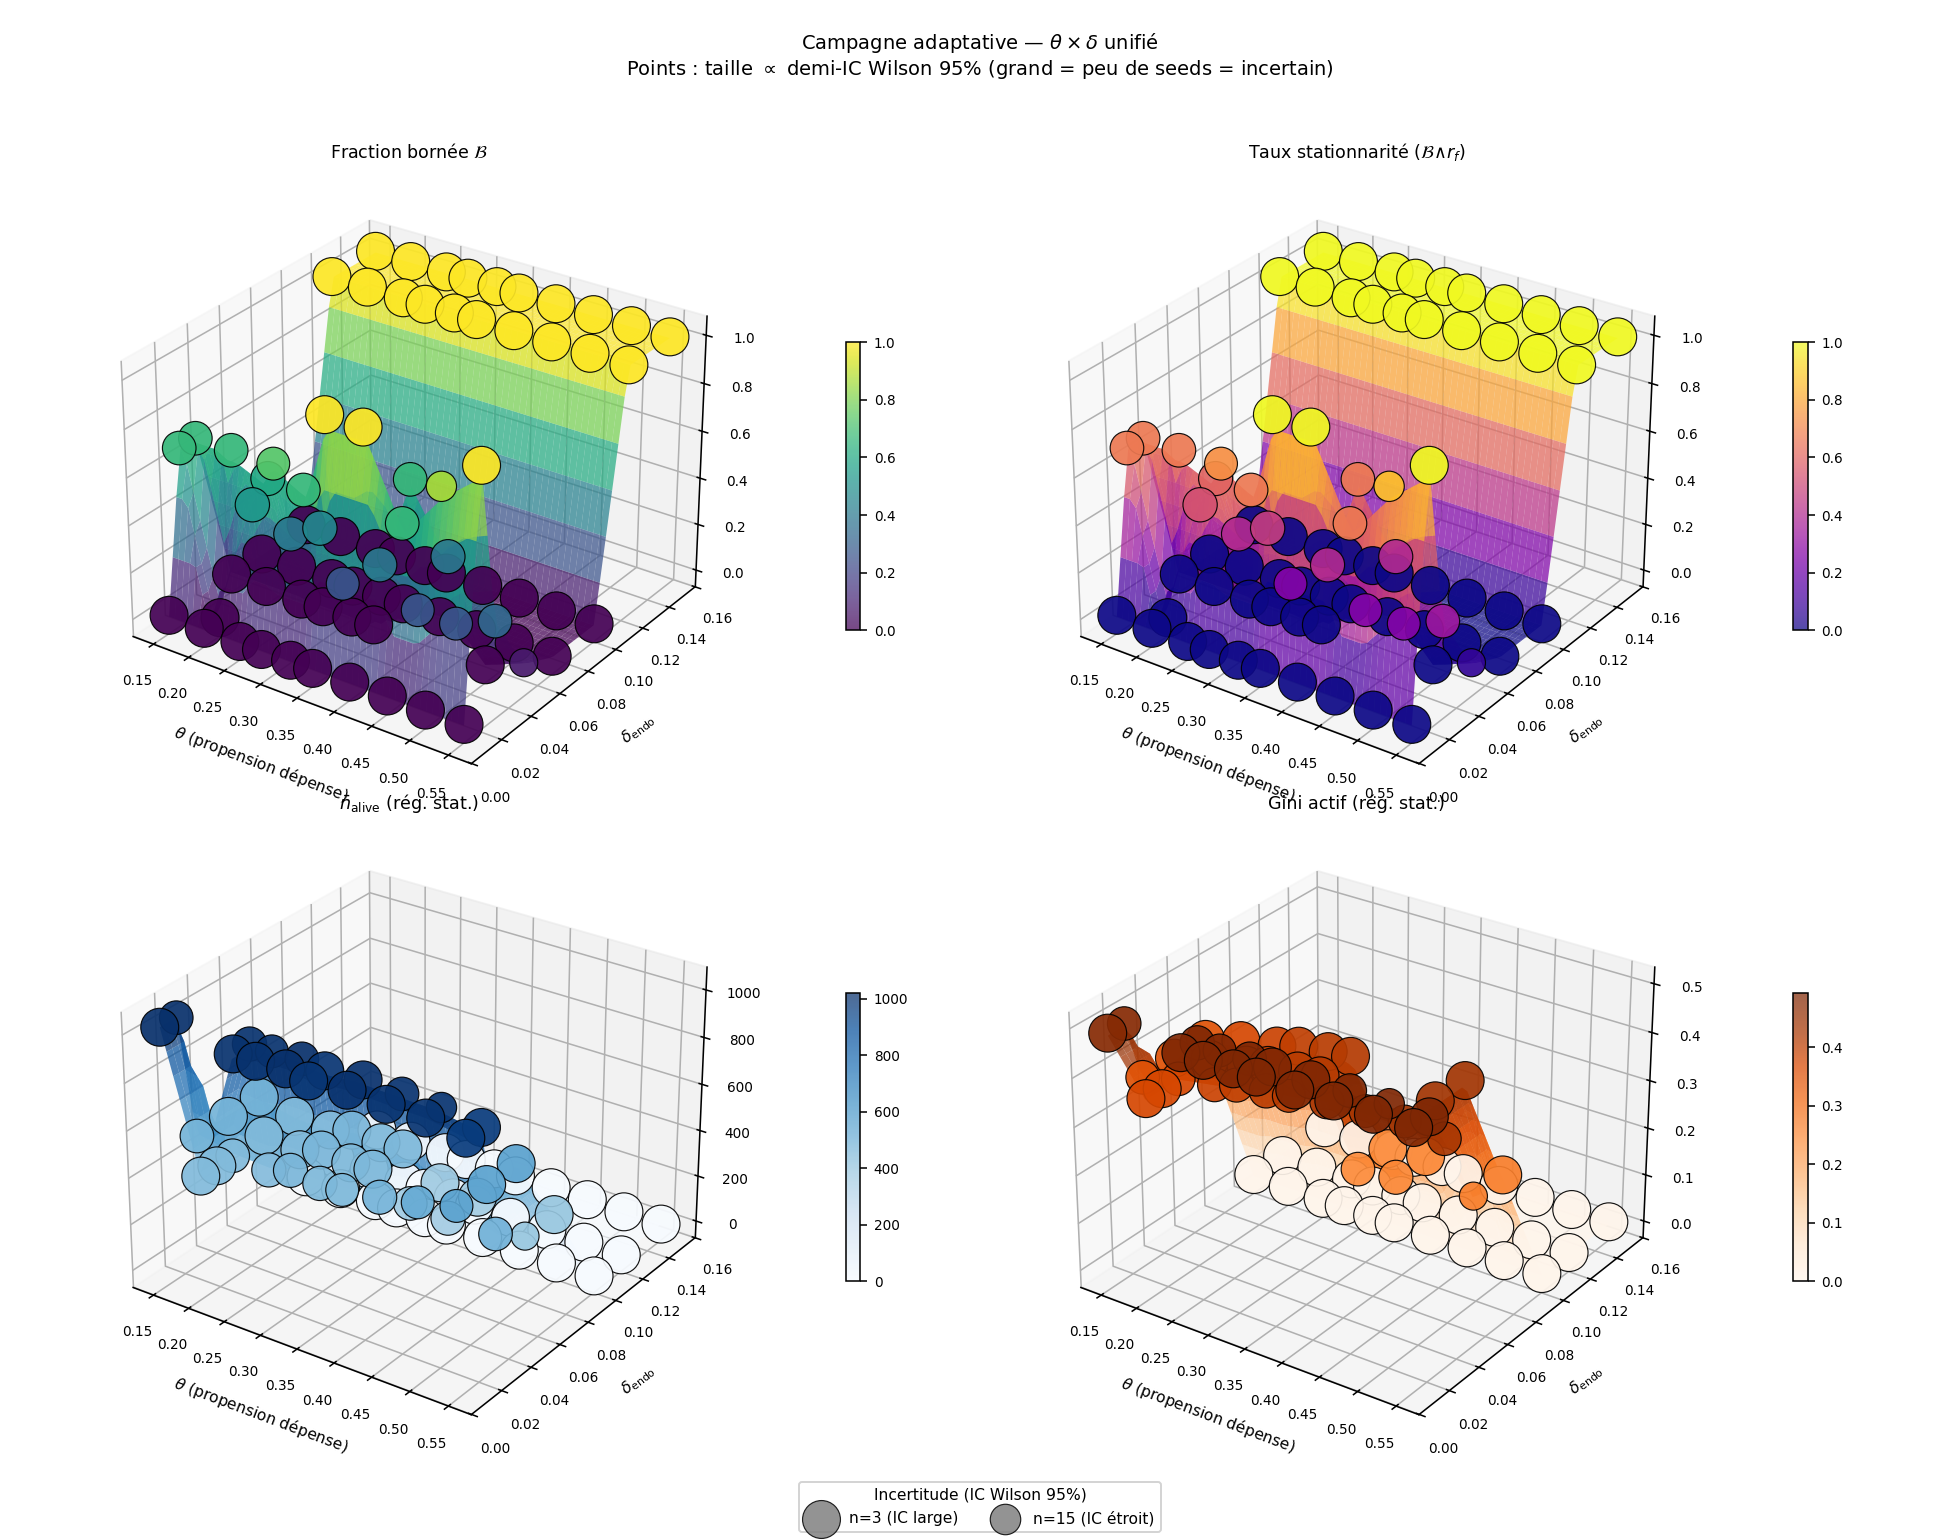
\includegraphics[width=\linewidth]{figures/map_theta_delta_3d.png}
  \caption{Cartes 3D adaptatives \(\theta \times \delta\) unifie (468 runs, 1500 pas)
  en disposition 2\(\times\)2.
  Points superposes : taille $\propto$ demi-IC Wilson 95\%.
  \textbf{Attention :} les points a \(\delta \ge 0.12\) (fraction 1.00 dans les
  panneaux \(\mathcal{B}\) et stationnarite) sont un \emph{artefact d'extinction}
  (\(n_{\mathrm{alive}} \approx 0\), variance nulle) et non un regime actif.
  Le veritable regime actif est restreint a \(\delta \in \{0.02, 0.03\}\),
  visible dans les panneaux \(\bar{n}_{\mathrm{alive}}\) et Gini (bas).}
\end{figure}

\textbf{Mise en garde critique : le motif haute-\(\delta\) est un artefact d'extinction.}
La table montre un motif non-monotone frappant : pour \(\delta \ge 0.12\),
la fraction converge est 1.00 pour tout \(\theta\), alors qu'elle est nulle ou
faible a \(\delta = 0.05\)--\(0.10\).
L'inspection directe des runs \(\delta \ge 0.12\) revele \(n_{\mathrm{alive}} \approx 0\)
et \(\texttt{densite\_fin} \approx 0\) : le systeme s'effondre rapidement.
La criterion \texttt{bounded\_tail} est satisfaite parce que la serie de population
est quasi constante a zero (variance nulle), non parce qu'il y a un regime actif.
Le critere dual (equilibre de flux) ne filtre pas cet artefact car le flux de faillites
est aussi proche de zero dans un systeme depopule.

\textbf{Il faut donc distinguer deux regions de la carte \(\theta \times \delta\) :}
\begin{itemize}
  \item \emph{Regime actif} : \(\delta \in [0.02, 0.03]\), fraction 0.27--1.00 selon \(\theta\).
    \(n_{\mathrm{alive}} \in [400, 1130]\), \(d_f \in [0.35, 0.43]\),
    loans/entite \(\approx 40\)--\(73\).
    C'est le veritable regime economique ; les frontieres sont stochastiques.
  \item \emph{Extinction rapide} : \(\delta \ge 0.12\), fraction 1.00.
    \(n_{\mathrm{alive}} \approx 0\), reseau absent.
    La queue est bornee par zero, non par un regime.
    \textbf{Ne pas interpreter comme un regime}.
\end{itemize}

\textbf{Resultats robustes du regime actif.}
La fenetre du regime actif est etroite en \(\delta\) : entre 0.02 et 0.03.
\(\delta = 0.01\) (tres faible friction) empeche la formation du regime pour tout \(\theta\),
et \(\delta = 0.05\)--\(0.10\) le detruit.
\(\theta\) a un effet modere dans la fenetre active : la frontiere
\(\theta\)-optimale se situe autour de 0.28--0.40 (\(\delta=0.02\)),
avec une fraction 0.67--1.00.
Ce resultat suggere une contrainte conjointe : le systeme a besoin d'une
friction moderee pour stabiliser les faillites, mais pas d'une friction trop
elevee qui epuise les bilans avant la formation du reseau.

\subsection*{Synthese des campagnes adaptatives}

\begin{table}[H]
\centering
\small
\begin{tabular}{lrrrrrr}
\toprule
Campagne & Runs & Converges & \(\bar{d}_f\) & \(\bar{n}_{\mathrm{alive}}\) & \(\overline{\mathrm{loan}/n}\) & \(\bar{G}\) \\
\midrule
\(\lambda \times k\) & 417 & 212 (51\%) & 0.236 & 368 & 10.4 & 0.226 \\
\(k \times \mu\)     & 327 & 157 (48\%) & 0.243 & 292 & 19.2 & 0.230 \\
\(\sigma_\alpha \times k\) & 267 & 91 (34\%) & 0.272 & 280 & 16.1 & 0.309 \\
\(\theta \times \delta\) (actif seul., \(\delta\in\{0.02,0.03\}\)) & 468 & 136 actifs & 0.387 & 706 & 55.0 & 0.432 \\
\bottomrule
\end{tabular}
\caption{Statistiques agregees des runs bornes dans les campagnes adaptatives.
$\bar{d}_f = \overline{V/A}$ = densite financiere en volume, moyenne sur les
runs bornes de la campagne.
$\bar{n}_{\mathrm{alive}}$ = population moyenne.
$\overline{\mathrm{loan}/n}$ = prets par entite vivante (\(\ell\)).
$\bar{G}$ = coefficient de Gini de l'actif entre entites, moyenne sur les runs
bornes.
La ligne \(\theta \times \delta\) exclut les extinctions (\(\delta \ge 0.12\))
et ne retient que les 136 runs bornes du regime actif (\(\delta \in \{0.02, 0.03\}\),
seules valeurs de \(\delta\) produisant des regimes bornes dans cette campagne).}
\end{table}

\textbf{Observations transversales.}
\begin{itemize}
  \item La densite financiere \(d_f\) est stable entre 0.24 et 0.27 dans les trois
    premieres campagnes, suggerant qu'elle est une \emph{propriete emergente robuste}
    du regime borne, peu sensible aux parametres de connectivite ou a \(\mu\).
    Elle est plus elevee dans la campagne \(\theta\times\delta\) active (0.39),
    possiblement parce que \(\delta\) faible limite la depreciation de l'actif et
    augmente le ratio.
  \item Le coefficient de Gini est significativement plus eleve dans la campagne
    \(\sigma_\alpha \times k\) (0.31 vs. 0.22--0.23 ailleurs), suggerant que
    la volatilite du rendement produit une concentration plus marquee.
    Ce resultat est fragile (91 runs seulement).
  \item Le taux de faillite est remarquablement stable autour de \(2.0\)--\(2.8\)
    dans toutes les campagnes, ce qui est coherent avec l'equilibre de flux :
    dans le regime borne, le nombre de faillites par pas egale approximativement
    \(\lambda_{\mathrm{creation}}\) (taux de naissance des nouvelles entites).
\end{itemize}

\section{Probabilites de regime : cas limites multi-seeds}
\label{sec:multirun}

Les cas classes comme \emph{instables inter-seeds} dans la campagne OAT
(section~\ref{sec:oat-robustesse}) ont ete simules avec 13 seeds
supplementaires (200--212) pour estimer la probabilite de regime bornee.

\begin{table}[H]
\centering
\small
\begin{tabular}{lrrrl}
\toprule
Cas & bornés / seeds & \(p_{\mathrm{regime}}\) & IC 95\% & interpretation \\
\midrule
\texttt{k4\_theta05} & 12/13 & 0.92 & $\pm$0.15 & robuste \\
\texttt{k3\_sigma020} & 12/13 & 0.92 & $\pm$0.15 & robuste \\
\texttt{k3\_actif100} & 9/13  & 0.69 & $\pm$0.25 & probable \\
\texttt{k4\_lam120}   & 6/13  & 0.46 & $\pm$0.27 & frontiere \\
\texttt{k4\_lam100}   & 4/13  & 0.31 & $\pm$0.25 & improbable \\
\texttt{k3\_sigma005} & 3/13  & 0.23 & $\pm$0.23 & improbable \\
\texttt{k4\_depr002}  & 2/13  & 0.15 & $\pm$0.20 & tres improbable \\
\bottomrule
\end{tabular}
\caption{Probabilites de regime estimees sur 13 seeds extra.
\texttt{k4\_depr002} et \texttt{k3\_sigma005} sont structurellement
peu susceptibles d'atteindre le regime a 1500 pas.
\texttt{k4\_theta05} etait 1/3 sur seed 42 par malchance.}
\end{table}

Ces resultats corrigent deux lectures de la campagne OAT :
\begin{itemize}
  \item \texttt{k4\_depr002} (\(\delta_{\mathrm{endo}}=0.02\)) etait compte
  comme un effet densifiant. En realite sa probabilite de regime est 0.15 :
  la perturbation place le systeme tres pres de la frontiere, pas au centre ;
  \item \texttt{k4\_theta05} semblait fragile (1/3 seeds) mais est en fait
  robuste (0.92) : le seed 42 etait un cas defavorable isolee.
\end{itemize}

\section{Dynamique transitoire de \(k=3, \sigma_\alpha=0.005\) : convergence a 10\,000 pas}
\label{sec:explosion-k3}

La sonde longue de la section precedente indiquait que \(k=3, \sigma_\alpha=0.005\)
restait non borne a 3000 pas. Une premiere extension a 5000 pas (watchdog 300 ms/pas)
avait suggere une oscillation soutenue sans convergence. Une extension supplementaire
a 10\,000 pas (watchdog 400 ms/pas), sur 6 seeds distinctes, revele que ce comportement
est \emph{transitoire} : la quasi-totalite des seeds atteignent la stationnarite.

\subsection*{Sonde 5000 pas (donnees historiques)}

\begin{table}[H]
\centering
\small
\begin{tabular}{rrrrl}
\toprule
Seed & Pas realises & \(n_{\mathrm{alive}}\) final & Prets actifs & Note \\
\midrule
42  & 1401 & 2096 & 11551 & arret watchdog (417 ms/pas) \\
7   & 5000 &  878 &  8720 & oscillation, avg 67 ms/pas \\
123 & 5000 & 1184 &  8863 & oscillation, avg 68 ms/pas \\
0   & 5000 &  885 & 11597 & oscillation, avg 78 ms/pas \\
1   & 5000 & 1199 &  8560 & oscillation, avg 69 ms/pas \\
\bottomrule
\end{tabular}
\caption{Long run \(k=3, \sigma_\alpha=0.005\) a 5000 pas -- donnees historiques.
Seed 42 s'arrete a 1401 pas (watchdog 300 ms/pas). Les 4 autres seeds atteignent 5000 pas
et presentent des oscillations de population sans atteindre le critere de stationnarite
(\texttt{bounded\_tail=True}).
L'absence de convergence a 5000 pas reflete un transitoire long, non un regime permanent.}
\label{tab:long-run-5k}
\end{table}

\begin{figure}[H]
  \centering
  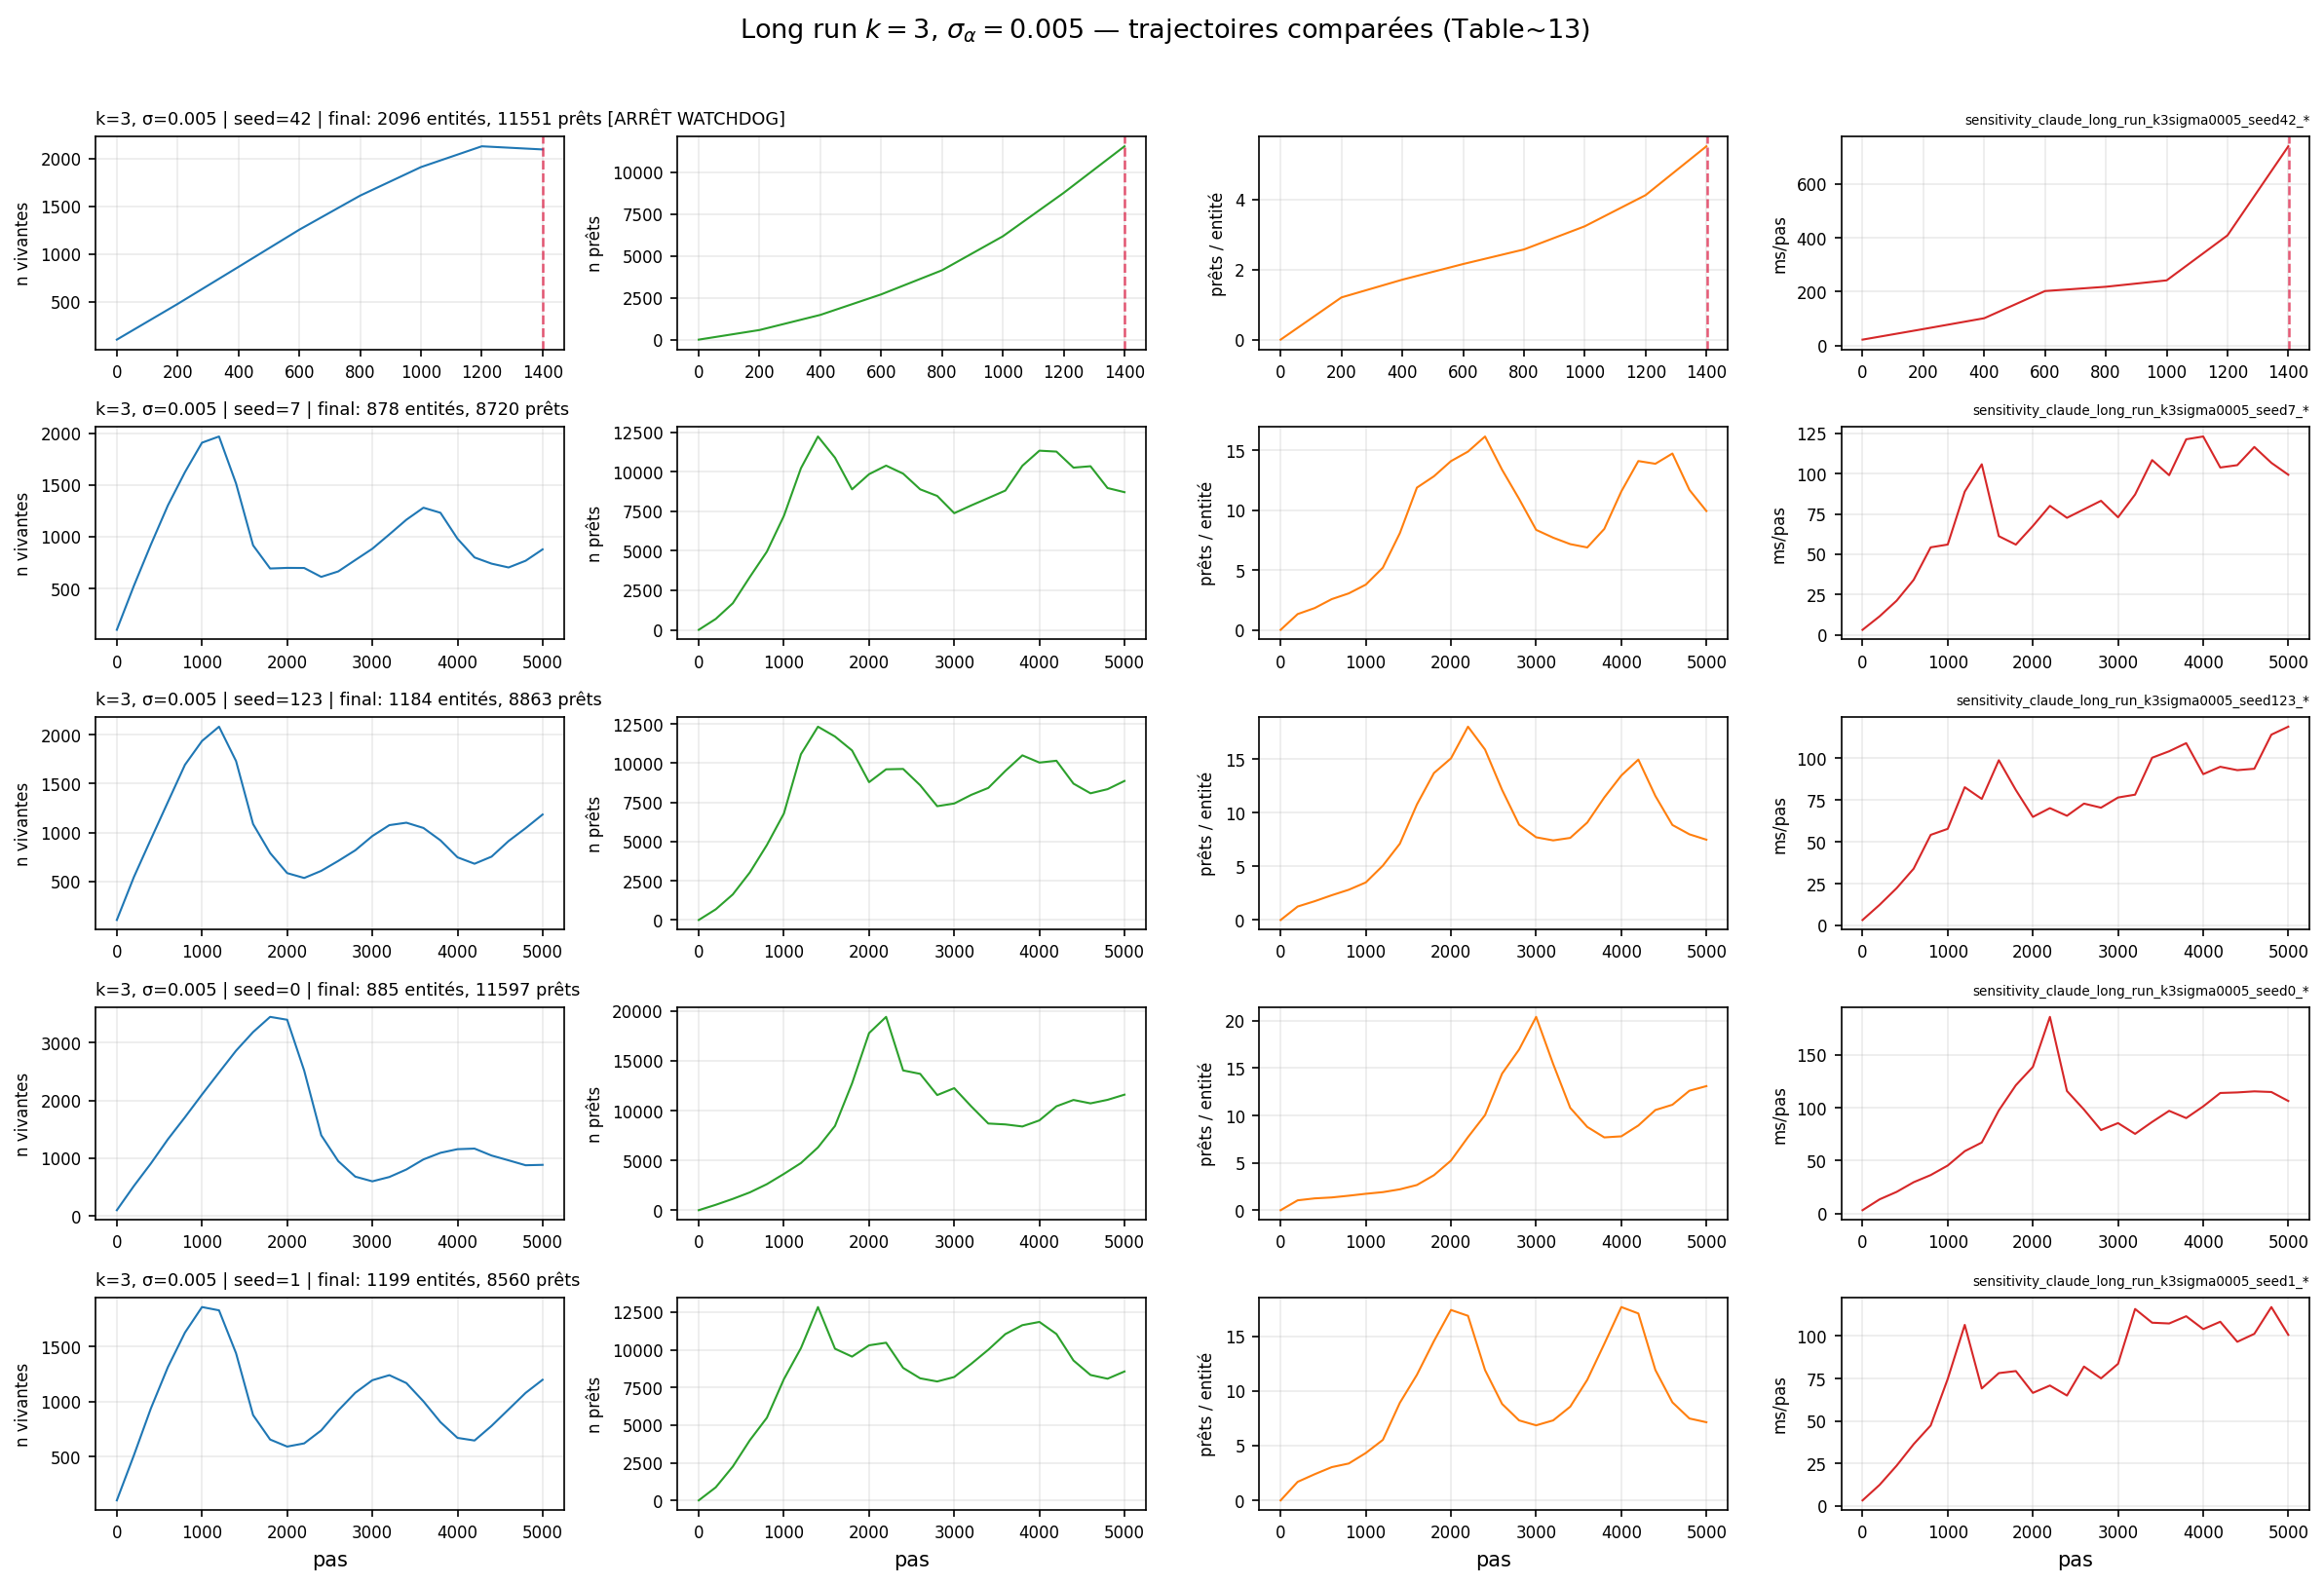
\includegraphics[width=0.98\linewidth]{figures/claude_long_run_k3sigma0005_trajectoires.png}
  \caption{Trajectoires comparees -- long run \(k=3,\,\sigma_\alpha=0.005\) a 5000 pas, 5 seeds.
  Colonnes : n vivantes (bleu), n prets (vert), densite prets/entite (orange), temps par pas en ms (rouge).
  La ligne verticale pointillee (seed 42) marque l'arret watchdog a 1401 pas.
  Les 4 autres seeds presentent des oscillations qui se revelent transitoires (voir Table~\ref{tab:long-run-10k}).}
\end{figure}

\subsection*{Extension a 10\,000 pas}

La meme configuration est simulee sur 6 seeds jusqu'a 10\,000 pas (execution sequentielle,
watchdog 400 ms/pas ; seed 42 exclue, divergence connue). La metrique de flux
\(\texttt{failure\_lambda\_ratio} = \bar{\mathcal{F}} / \lambda\) mesure le rapport entre
le taux de faillite moyen (fenetre de queue) et le taux de creation \(\lambda=2\) ;
la condition \(|r_f - 1| < 0.15\) (\texttt{failure\_lambda\_ratio}) definit l'equilibre des flux
(voir section~\ref{sec:critere-regime}).

\begin{table}[H]
\centering
\small
\begin{tabular}{rrrrrll}
\toprule
Seed & Pas & \(n_{\mathrm{alive}}\) final & $r_f$ & ms/pas moy. & $\mathcal{B}$ & Statut \\
\midrule
7   & 10000 & 1191 & 1.011 & 121 & $\surd$ & stationnaire \\
123 & 10000 & 1025 & 0.966 & 121 & $\surd$ & stationnaire \\
0   & 10000 & 1244 & 0.994 & 135 & $\surd$ & stationnaire \\
1   & 10000 &  812 & 0.984 & 129 & $\surd$ & stationnaire \\
2   & 10000 &  942 & 0.985 & 126 & $\times$ & flux OK, non borne \\
3   & 10000 & 1104 & 1.010 & 123 & $\surd$ & stationnaire \\
\bottomrule
\end{tabular}
\caption{Long run \(k=3, \sigma_\alpha=0.005\) a 10\,000 pas -- 6 seeds (seed 42 exclue).
$\mathcal{B}$ = \texttt{bounded\_tail} (critere de queue).
$r_f = \bar{f}/\lambda$ = taux faillites / creation (\texttt{failure\_lambda\_ratio}).
5 seeds sur 6 sont stationnaires (\(\mathcal{B}\) ET \(|r_f-1|<0.15\)).
Tous les $r_f$ sont dans \([0.966 ; 1.011]\), indiquant un equilibre presque parfait entre creations
et faillites. Seed 2 : flux equilibre mais queue non bornee -- cas limite.}
\label{tab:long-run-10k}
\end{table}

\begin{figure}[H]
  \centering
  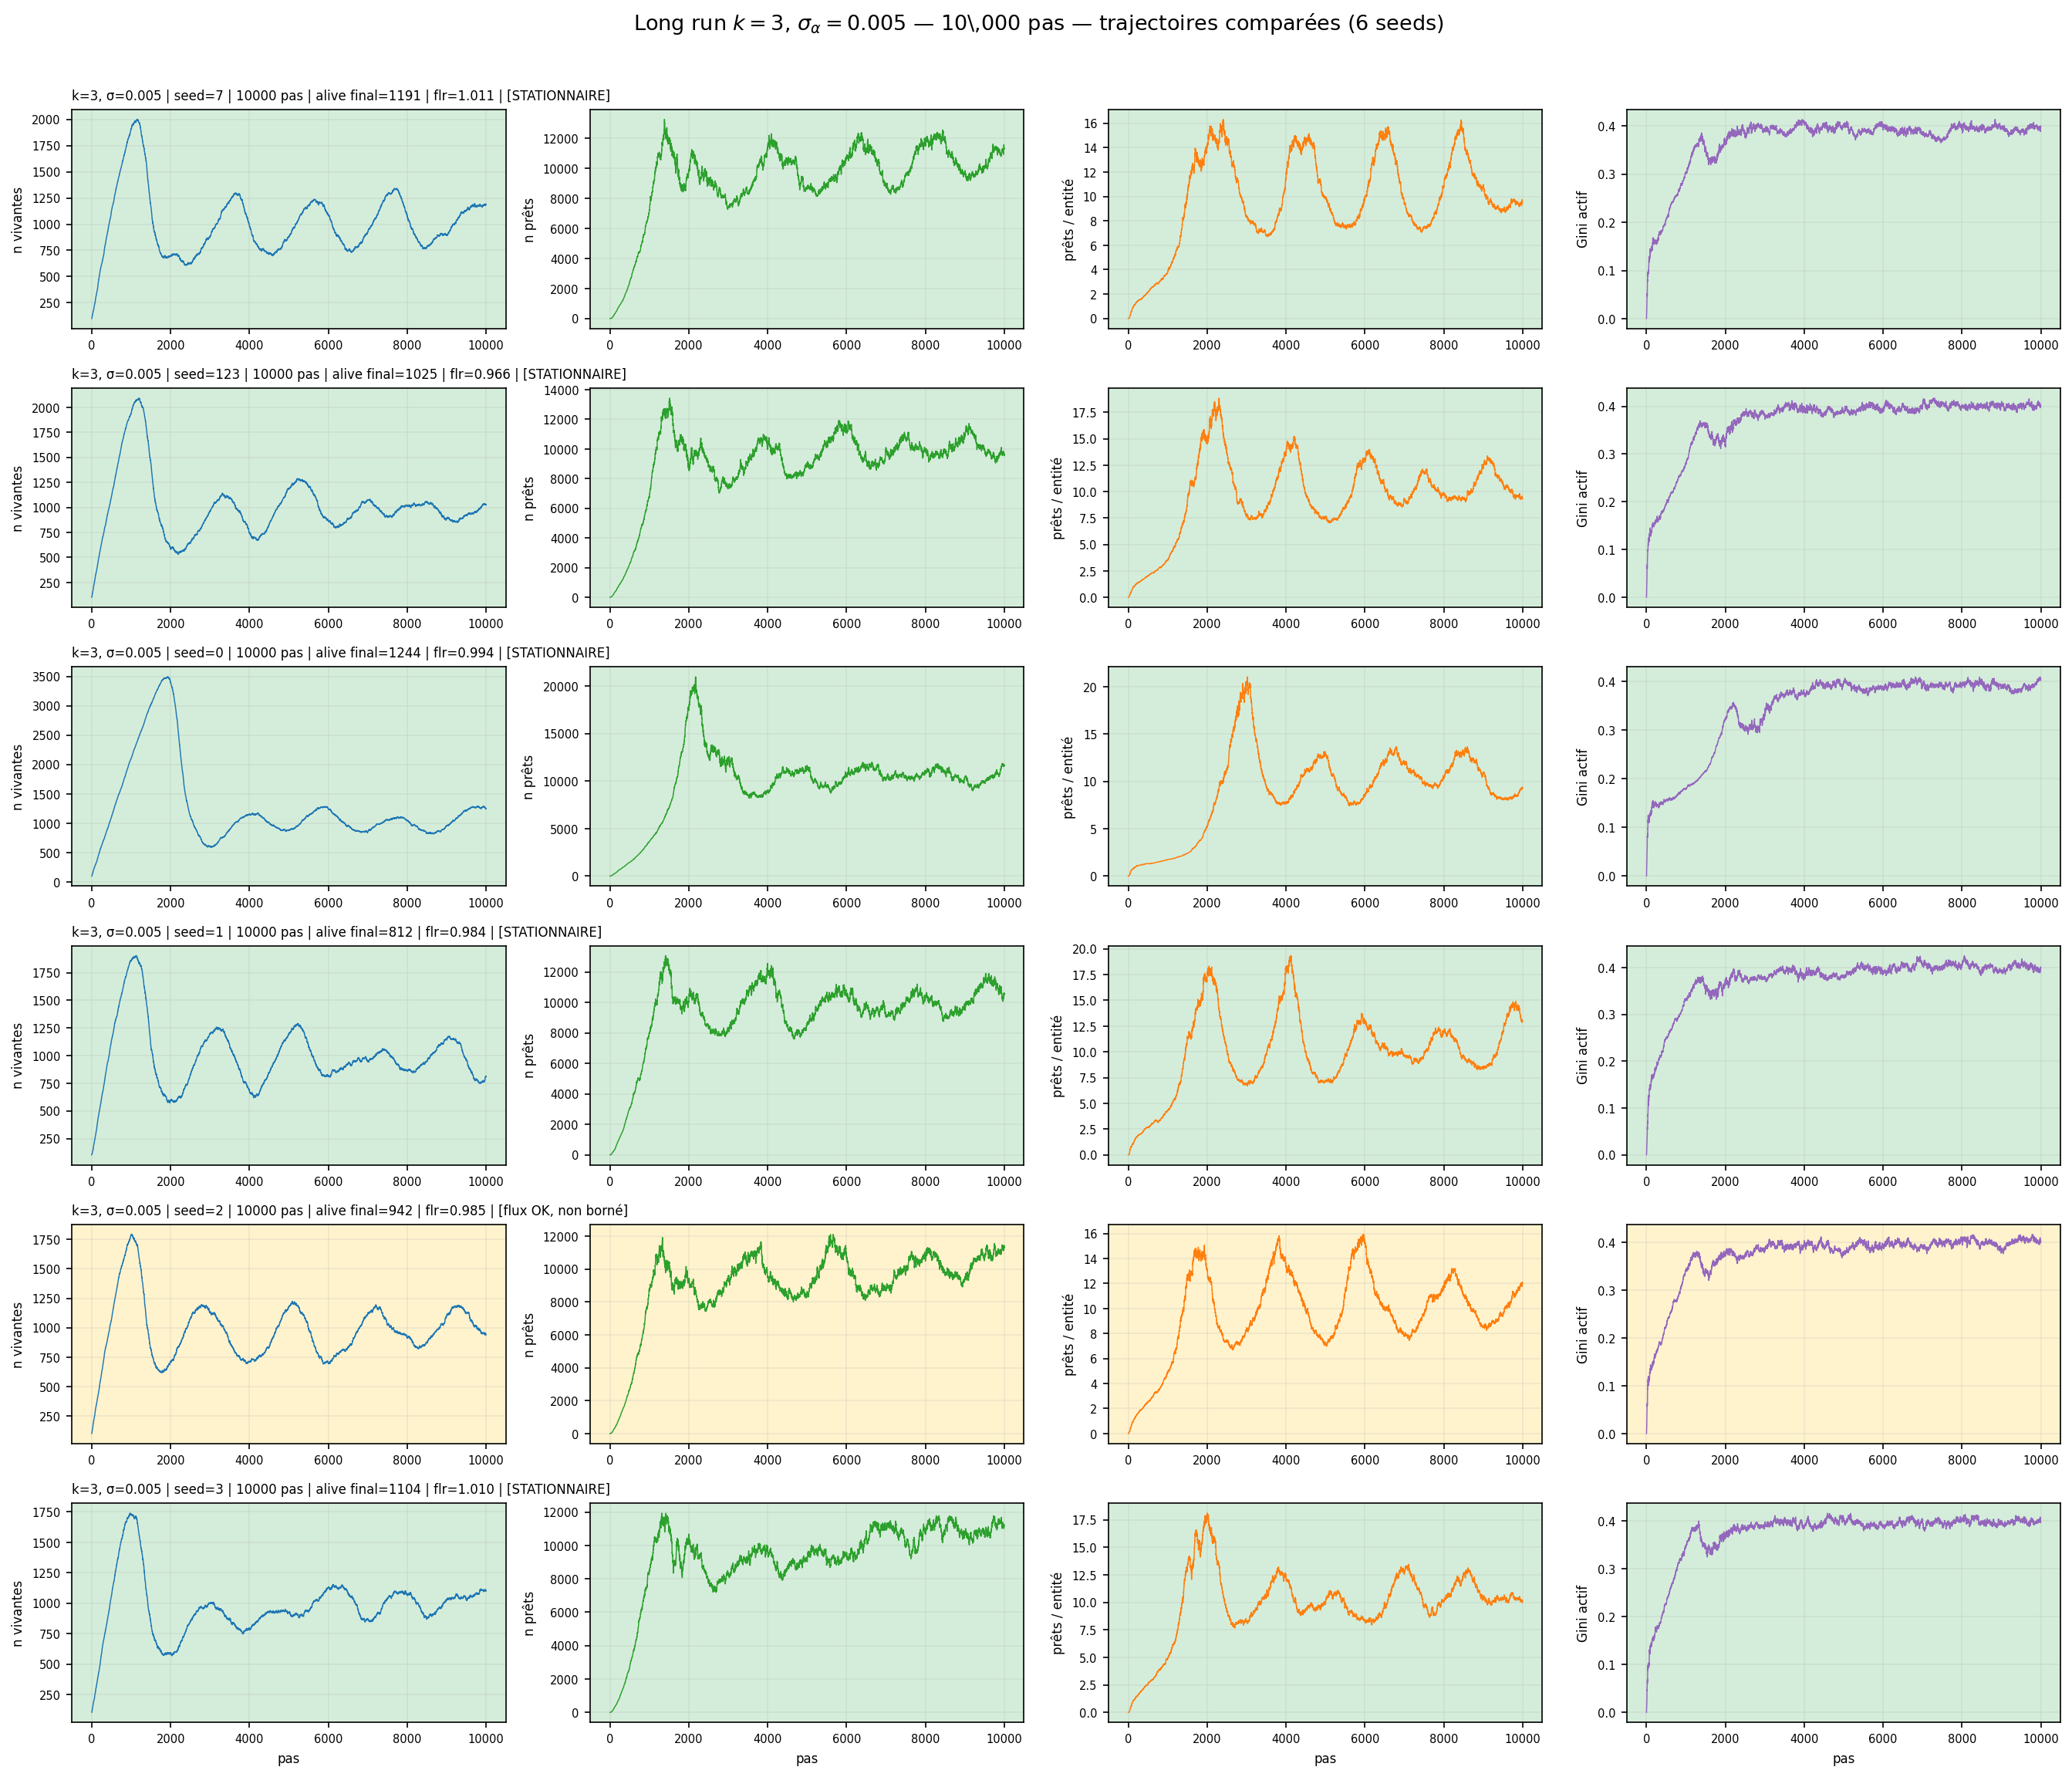
\includegraphics[width=0.98\linewidth]{figures/long_run_k3sigma0005_10k_trajectoires.png}
  \caption{Trajectoires comparees -- long run \(k=3,\,\sigma_\alpha=0.005\) a 10\,000 pas, 6 seeds.
  Colonnes : n vivantes (bleu), n prets (vert), densite prets/entite (orange), Gini actif (violet).
  Fond vert : seed stationnaire ; fond jaune : seed non-stationnaire (seed 2 uniquement).
  Toutes les trajectoires se stabilisent apres 4000--6000 pas.}
\end{figure}

Le comportement de \(k=3, \sigma_\alpha=0.005\) est desormais clarifie : les oscillations
observees a 5000 pas sont un \emph{transitoire} d'une duree de l'ordre de 4000--6000 pas,
non un regime permanent. Apres ce transitoire, 5 seeds sur 6 convergent vers un regime
borne et en equilibre de flux. La seed 2 constitue un cas limite ou le flux est equilibre
mais la queue de population reste non bornee.

La probabilite de regime de 0.23 mesuree en section~\ref{sec:multirun} (13 seeds, 1500 pas)
doit donc etre reinterpretee comme une probabilite de \emph{convergence rapide} plutot que
de stationnarite asymptotique : la grande majorite des seeds convergent, mais sur un horizon
long (\(\sim\)5000--10000 pas). Sur l'horizon court des multi-runs, seule une minorite
presente un regime borne detectable.

\section{Parametres faibles : mecanismes candidats a la suppression}
\label{sec:parametres-faibles}

La campagne OAT avec 3 seeds et les couplages ont permis d'identifier deux
parametres dont l'effet mesure est exactement nul sur \textbf{toutes} les
metriques (densite financiere, \(n_{\mathrm{alive}}\), \texttt{bounded\_tail})
dans les deux centres et les deux directions :

\begin{itemize}
  \item \texttt{coefficient\_reliquefaction} : decote a la cession forcee
  lors de la liquidation. Valeur par defaut : 0.5. Aucun delta mesure ;
  \item \texttt{seuil\_ratio\_liquide\_passif} : seuil de declenchement de
  la reliquefaction. Valeur par defaut : 0.05. Aucun delta mesure.
\end{itemize}

Ces deux parametres decrivent le mecanisme de reliquefaction. Leur absence
d'effet suggere que ce mecanisme n'est pas active sur les horizons et les
regimes testes, ou qu'il est redondant avec d'autres voies de liquidation.
Ils sont \textbf{candidats prioritaires a la suppression} pour simplifier
le modele, sous reserve d'une verification analytique.

\section{Predictabilite des series temporelles par regime}
\label{sec:predictabilite}

\subsection*{Définitions des indicateurs}

Les quatre indicateurs ci-dessous sont calculés sur la serie temporelle
$n_{\mathrm{alive}}(t)$, prise en differences premieres $\Delta n_t = n_{t+1} - n_t$
(sauf indication contraire).

\paragraph{Exposant de Hurst $H$ (analyse R/S).}
Soit une fenetre de longueur $\ell$ de la serie. On calcule le rapport
$R/S$ : etendue de la somme cumulee des ecarts a la moyenne, divisee par
l'ecart-type de la fenetre. L'exposant $H$ est la pente de $\log(R/S)$
en fonction de $\log(\ell)$. Pour un bruit blanc, $H = 0.5$~; une serie
avec memoire longue positive donne $H > 0.5$~; une serie anti-persistante
$H < 0.5$. \emph{Attention~: quand la serie est quasi-constante (extinction),
$R/S$ est numeriquement instable et la pente remonte artificiellement vers
$H \approx 2$. Dans ce cas, $H$ ne mesure plus la memoire mais un artefact
de variance nulle~; seul $S_p$ est alors pertinent.}

\paragraph{Autocorrelation au lag 20 ($r_{20}$).}
Correlation de Pearson de $n_t$ avec $n_{t-20}$ sur la totalite de la serie.
$r_{20} \approx 0$ indique l'absence de dependance a l'horizon de 20 pas~;
$r_{20} > 0$ une tendance persistante (la population dans 20 pas depend de
l'etat present)~; $r_{20} < 0$ un comportement oscillatoire ou reversif.

\paragraph{Ratio MSE AR(5) / predicteur naif.}
On ajuste un modele autoregressif d'ordre 5 (AR(5)) sur la serie
$n_{\mathrm{alive}}$ et on mesure son erreur quadratique moyenne (MSE) sur
un pas d'horizon en validation croisee. Le predicteur naif est $\hat{n}_{t+1}
= n_t$ (valeur actuelle reconduite). Le ratio AR(5)/naif~$> 1$ signifie que
le modele AR n'apporte aucun avantage sur la reconduite~; un ratio~$< 1$
signifie qu'exploiter la memoire courte des 5 derniers pas ameliore la
prediction.

\paragraph{Entropie de permutation $S_p$ (ordre 3).}
Pour chaque triplet de valeurs consecutives $(n_t, n_{t+1}, n_{t+2})$, on
extrait uniquement le patron d'ordre relatif : parmi les $3! = 6$ permutations
possibles (ascendant-ascendant, ascendant-descendant, etc.), on denombre la
frequence d'apparition de chacun sur la serie entiere, puis on calcule
l'entropie de Shannon normalisee~:
\[
  S_p = -\frac{1}{\log_2 6} \sum_{i=1}^{6} p_i \log_2 p_i \;\in [0, 1].
\]
$S_p \approx 0$ indique que tous les triplets ont le meme patron (serie
monotone ou plate)~; $S_p = 1$ indique que tous les patrons sont
equiprobables (fluctuations maximalement impredictibles pas-a-pas). $S_p$
ne depend pas de l'amplitude des valeurs, seulement de leur structure locale.

\bigskip
L'analyse a ete conduite sur 10 cas de test (3~seeds chacun,
1500 pas) et sur 8 runs longs issus de la sonde codex (3000 pas, seed~42).

\begin{table}[h]
\centering
\small
\begin{tabular}{lccccl}
\hline
Cas & $H$ & $r_{20}$ & AR/naif & $S_p$ & Classe \\
\hline
k2\_baseline         & 1.993 & $-0.01$ & 0.62 & 0.00 & régime\_structuré \\
k3\_baseline         & 1.990 & $+0.01$ & 0.60 & 0.00 & régime\_structuré \\
k4\_actif400\_exit   & 1.993 & $-0.00$ & 0.62 & 0.00 & régime\_structuré \\
k4\_theta02\_exit    & 1.994 & $+0.00$ & 0.58 & 0.00 & régime\_structuré \\
k4\_lambda4\_growth  & 1.988 & $-0.00$ & 0.43 & 0.02 & régime\_structuré \\
\hline
k3\_sigma005         & 1.939 & $+0.40$ & 0.88 & 0.54 & variation\_lente \\
k4\_lam30            & 1.970 & $+0.54$ & 0.76 & 0.73 & variation\_lente \\
\hline
k3\_mu0              & 1.523 & $+0.12$ & 1.05 & 0.89 & tendance\_modérée \\
k3\_sigma020         & 1.577 & $+0.15$ & 1.06 & 0.83 & tendance\_modérée \\
k4\_baseline         & 1.480 & $+0.28$ & 1.08 & 0.84 & tendance\_modérée \\
k4\_sigma020         & 1.603 & $+0.12$ & 1.06 & 0.87 & tendance\_modérée \\
k5\_baseline         & 1.545 & $+0.21$ & 1.08 & 0.86 & tendance\_modérée \\
\hline
\end{tabular}
\caption{Metriques de predictabilite par cas. $H$~: Hurst R/S ; $r_{20}$~: autocorrelation
au lag~20 ; AR/naif~: ratio MSE AR(5) / naif (>1 = AR no better) ; $S_p$~: entropie de
permutation. Les cas \texttt{bounded} (\(p \ge 0.67\)) apparaissent en zone tendance\_modérée.}
\end{table}

Trois classes emergent :

\begin{enumerate}
  \item \textbf{Régime structuré / extinction} (H~$\approx$~2, $S_p \approx 0$, AR/naif~$<$~1).
    La serie de $n_{\mathrm{alive}}$ converge vers un quasi-point fixe ou une oscillation
    reguliere, de variance quasi nulle. L'entropie de permutation s'annule, le ratio AR/naif
    descend sous 1 (la memoire locale aide a predire). Ce comportement caracterise les cas
    d'extinction ($k \le 3$ sans perturbation, ou $k=4$ avec $\theta$ ou $\delta$ extremes).
    \textit{Note~: les valeurs $H>1$ obtenues par R/S sur des series quasi-constantes sont
    des artefacts numeriques ; l'indicateur pertinent est $S_p$.}

  \item \textbf{Variation lente / explosion} (H~$\approx$~1.9-2.0, $r_{20} \approx 0.4$-$0.5$).
    Une autocorrelation longue portee domine. La population croit sans borne (k3\_sigma005,
    k4\_lam30), la tendance absorbe le signal stochastique.

  \item \textbf{Tendance moderee / regime borne} (H~$\approx$~1.5, $S_p \approx 0.85$,
    AR/naif~$>$~1). Les cas bornes se regroupent ici. L'entropie de permutation est haute~:
    la sequence des fluctuations est quasi-aleatoire pas-a-pas, AR(5) ne bat pas le predicteur
    naif. Le regime borne est donc le \textbf{moins predictible a court terme} -- ce qui est
    coherent avec une fluctuation d'equilibre structurel.
\end{enumerate}

\textbf{Corollaire pratique.} L'entropie de permutation $S_p$ est le meilleur separateur
des trois classes sur un seul scalaire : $S_p < 0.1$ signale l'extinction, $S_p \in [0.4, 0.75]$
l'explosion, $S_p > 0.80$ le regime borne. L'exposant de Hurst a lui seul est insuffisant~:
les regimes d'extinction et d'explosion partagent tous deux $H \approx 2$.

\section{Ce qui reste a eclairer}

Plusieurs zones restent ouvertes apres les campagnes adaptatives.

Premierement, les fluctuations non-monotones dans les cartes \(k\times\mu\)
et \(\sigma_\alpha\times k\) (zones de fraction alternant 0.00 et 0.40--0.67
dans des ranges contigus) peuvent refleter des effets de front de phase ou des
artefacts du petit echantillon aux frontieres. Un echantillon supplementaire
ciblant ces cellules (au moins 15 seeds) permettrait de trancher.

Deuxiemement, la campagne \(\theta\times\delta\) unifiee montre que le regime
actif est limite a \(\delta \in [0.02, 0.03]\). La frontiere basse (\(\delta=0.01\)
toujours non borne) n'a pas de mecanisme interprete : pourquoi une friction trop
faible empeche-t-elle la formation du regime ? Une analyse de la dynamique de
creation/destruction a \(\delta=0.01\) serait utile.

Troisiemement, la distribution des tailles d'entites en regime permanent
n'a pas ete analysee en detail. Les metriques Gini et snapshots existent dans
les runs Simulation Lab, mais une comparaison lognormale / Pareto / melange
de regimes demanderait une extraction dediee des distributions finales des
runs bornes.

\section{Conclusion}

Le comportement du modele est predictible a gros traits depuis les parametres,
mais pas par une loi lineaire simple. Les variables les plus structurantes sont
des variables de seuil : \(k\), \(\sigma_\alpha\), \(\theta\), \(\mu\),
\(\lambda\), les depreciations et la dotation initiale.

Les campagnes adaptatives (1\,479 runs au total) confirment et precisent
la geometrie de la surface de regime.
\(\mu\) (prime minimale a l'emprunt) apparait comme un co-facteur de seuil
independant : \(\mu=0\) permet au modele d'entrer en regime meme a \(k=2\),
ce qui reinterprete les resultats du balayage \(k\) comme dependant implicitement
du choix \(\mu=0.05\). La frontiere \(k=3 \to k=4\) n'est pas absolue :
c'est la combinaison \((k, \mu)\) qui determine si le marche du credit est
suffisamment actif.

La depreciation unifiee \(\delta\) se revele etre un parametre a double effet :
dans la fenetre \([0.02, 0.03]\), elle stabilise le regime en fournissant une
friction moderee ; au-dela de 0.05, elle empeche systematiquement la formation
du regime ; au-dela de 0.12, elle provoque une extinction rapide qui satisfait
trivialement le critere de queue bornee. Ce troisieme regime (extinction) est
un artefact du critere de convergence et ne doit pas etre interprete comme
un regime economique.

\textbf{Propriete emergente robuste.}
La densite financiere en volume (\(d_f = \texttt{volume\_prets}/\texttt{actif\_total}\))
est stable a \(0.24 \pm 0.02\) dans les regimes actifs des campagnes \(\lambda\times k\)
et \(k\times\mu\), independamment des parametres de connectivite. Cette stabilite
suggere que \(d_f\) est une propriete emergente du regime, non un effet direct
des parametres.

Deux mecanismes du modele (reliquefaction) ont un effet nul mesure sur tous
les horizons testes et sont candidats a la suppression pour simplifier le
modele. Un regime dense demande un reseau de credit suffisamment actif pour
produire des faillites endogenes, mais pas une fragmentation numerique
excessive. Une population nombreuse n'est pas un signe de stabilite : dans
certains cas (notamment \(k=3, \sigma_\alpha=0.005\) sur des horizons courts),
elle signale un transitoire long avant la convergence -- non une instabilite permanente.
Pour predire finement une simulation, il faut donc predire conjointement :
apparition du regime, densite financiere en volume, granularite du reseau,
taille demographique, taille bilancielle et derive de queue.

\clearpage
\newgeometry{landscape, top=1.8cm, bottom=1.8cm, left=2cm, right=2cm}
\begin{landscape}
% Annexe de traçabilité — généré automatiquement le 2026-05-04
% Toute simulation mentionnée dans le rapport est listée ici avec son run_id.
% Le run_id permet de retrouver la simulation dans Simulation Lab.

\section*{Annexe~A — Traçabilité des simulations}
\addcontentsline{toc}{section}{Annexe A — Traçabilité des simulations}

Cette annexe recense toutes les simulations utilisées dans le présent rapport,
classées par usage. Chaque simulation est identifiée par son \texttt{run\_id}
unique dans Simulation Lab (\texttt{simulation\_lab\_data/runs/<run\_id>/run.json}).

Pour retrouver une simulation : ouvrir Simulation Lab, utiliser la barre de
recherche et saisir le hash (ou un préfixe).

\subsection*{A.1 Figures}

\begin{longtable}{p{0.22\linewidth}p{0.13\linewidth}p{0.34\linewidth}p{0.22\linewidth}}
\hline
\textbf{Figure} & \textbf{Seeds} & \textbf{Batch / Run ID (préfixe)} & \textbf{Statut} \\
\hline
\endfirsthead
\hline
\textbf{Figure} & \textbf{Seeds} & \textbf{Batch / Run ID (préfixe)} & \textbf{Statut} \\
\hline
\endhead
\hline
\endfoot

Fig.~1 — Corrélations pilote
 & 42 & \texttt{sensitivity\_lab\_guided\_probe} & external (meta.json) \\

Fig.~2 — Balayage $k$
 & 42 & \texttt{sensitivity\_k\_sweep\_*} (batch \texttt{k\_sweep}) & external \\

Fig.~3 — Compromis $\epsilon$
 & 42 & \texttt{sensitivity\_epsilon\_runtime\_*} & external \\

Fig.~4 — Fenêtre $\sigma_\alpha$
 & 42, 7, 123 & \texttt{sensitivity\_alpha\_sigma\_hom\_*} & external \\

Fig.~5 — OAT screen $k=4$, $k=3$
 & 42 & \texttt{sensitivity\_codex\_oat\_steps1500\_seeds42\_*} & external \\

Fig.~6 — Sonde longue 3000 pas
 & 42 & \texttt{sensitivity\_codex\_long\_probe\_steps3000\_seeds42\_*} & external \\

Fig.~7 — Planches OAT (Simulation Lab)
 & 42 & \texttt{sensitivity\_codex\_oat\_key\_figures} + batch \texttt{codex\_oat} & external \\

Fig.~8 — Importance prédictive
 & 42 & dérivé de \texttt{codex\_oat\_steps1500\_seeds42} (calcul ML) & calculé \\

Fig.~9 — Cartes de phase empiriques
 & 42 & dérivé des résultats OAT Codex & calculé \\

Fig.~10 — Balayage fin $\lambda$
 & 42, 7, 123 & \texttt{sensitivity\_claude\_lambda\_fine\_sweep\_*} & managed \\

Fig.~11 — Robustesse OAT
 & 42, 7, 123 & \texttt{sensitivity\_claude\_oat\_robustness\_*} & managed \\

\hline
\end{longtable}

\subsection*{A.2 Tables}

\begin{longtable}{p{0.18\linewidth}p{0.13\linewidth}p{0.38\linewidth}p{0.22\linewidth}}
\hline
\textbf{Table} & \textbf{Seeds} & \textbf{Batch / Run ID (préfixe)} & \textbf{Statut} \\
\hline
\endfirsthead
\hline
\textbf{Table} & \textbf{Seeds} & \textbf{Batch / Run ID (préfixe)} & \textbf{Statut} \\
\hline
\endhead
\hline
\endfoot

Table~1 — Balayage $k$
 & 42 & \texttt{sensitivity\_k\_sweep\_*} & external \\

Table~2 — OAT $k=4$ (effets bruts)
 & 42 & \texttt{sensitivity\_codex\_oat\_steps1500\_seeds42\_*} & external \\

Table~3 — Sonde longue 3000 pas
 & 42 & \texttt{sensitivity\_codex\_long\_probe\_steps3000\_seeds42\_*} & external \\

Table~4 — Balayage fin $\lambda$
 & 42, 7, 123 & \texttt{sensitivity\_claude\_lambda\_fine\_sweep\_*} & managed \\

Table~5 — Robustesse OAT centre $k=4$
 & 42, 7, 123 & \texttt{sensitivity\_claude\_oat\_robustness\_seed*} & managed \\

Table~6 — Robustesse OAT centre $k=3$
 & 42, 7, 123 & \texttt{sensitivity\_claude\_oat\_robustness\_seed*} & managed \\

Table~7 — Couplage $\lambda \times k$
 & 42, 7, 123 & \texttt{sensitivity\_ts\_coupling\_lambda\_k\_*} ou \texttt{sensitivity\_*\_coupling\_lambda\_k\_*} & managed \\

Table~8 — Couplage $k \times \mu$
 & 42, 7, 123 & \texttt{sensitivity\_ts\_coupling\_k\_mu\_*} & managed \\

Table~9 — Couplage $\sigma_\alpha \times k$
 & 42, 7, 123 & \texttt{sensitivity\_ts\_coupling\_sigma\_k\_*} & managed \\

Table~10 — Couplage $\theta \times \delta_{\mathrm{endo}}$
 & 42, 7, 123 & \texttt{sensitivity\_ts\_coupling\_theta\_depr\_*} & managed \\

Table~11 — Probabilités de régime (multi-seeds)
 & 13 seeds (42…12) & \texttt{sensitivity\_claude\_multirun\_limits\_*} & managed \\

Table~12 — Prédictabilité
 & 42 & \texttt{sensitivity\_codex\_oat\_steps1500\_seeds42\_*} + dérivé & calculé \\

Table~13 (5k) — Long run $k=3$, $\sigma_\alpha=0.005$, 5 seeds
 & 42, 7, 123, 0, 1 & \texttt{sensitivity\_claude\_long\_run\_k3sigma0005\_seed*} & managed \\

Table~13 (10k) — Long run $k=3$, $\sigma_\alpha=0.005$, 6 seeds à 10\,000 pas
 & 7, 123, 0, 1, 2, 3 & \texttt{sensitivity\_claude\_long\_run\_k3sigma0005\_10k\_seed*} & managed \\

\hline
\end{longtable}

\subsection*{A.3 Simulations de référence citées dans le texte}

\begin{longtable}{p{0.30\linewidth}p{0.10\linewidth}p{0.40\linewidth}p{0.12\linewidth}}
\hline
\textbf{Rôle / section} & \textbf{Paramètres clés} & \textbf{Run ID exact} & \textbf{Stat.} \\
\hline
\endfirsthead
\hline
\textbf{Rôle / section} & \textbf{Paramètres clés} & \textbf{Run ID exact} & \textbf{Stat.} \\
\hline
\endhead
\hline
\endfoot

Sonde longue — $k=3$, $\sigma=0.005$, seed 42 (Fig.~6, Table~13)
 & $k=3$, $\sigma=0.005$, seed=42
 & \texttt{sensitivity\_claude\_long\_run\_k3sigma0005\_seed42\_000}
 & stopped (1401 pas) \\

Sonde longue 5k — $k=3$, $\sigma=0.005$, seed 7 (Table~13)
 & $k=3$, $\sigma=0.005$, seed=7
 & \texttt{sensitivity\_claude\_long\_run\_k3sigma0005\_seed7\_001}
 & transitoire (non-stationnaire à 5k) \\

Sonde longue 5k — $k=3$, $\sigma=0.005$, seed 123 (Table~13)
 & $k=3$, $\sigma=0.005$, seed=123
 & \texttt{sensitivity\_claude\_long\_run\_k3sigma0005\_seed123\_002}
 & transitoire (non-stationnaire à 5k) \\

Sonde longue 5k — $k=3$, $\sigma=0.005$, seed 0 (Table~13)
 & $k=3$, $\sigma=0.005$, seed=0
 & \texttt{sensitivity\_claude\_long\_run\_k3sigma0005\_seed0\_003}
 & transitoire (non-stationnaire à 5k) \\

Sonde longue 5k — $k=3$, $\sigma=0.005$, seed 1 (Table~13)
 & $k=3$, $\sigma=0.005$, seed=1
 & \texttt{sensitivity\_claude\_long\_run\_k3sigma0005\_seed1\_004}
 & transitoire (non-stationnaire à 5k) \\

Long run 10k — $k=3$, $\sigma=0.005$, seed 7
 & $k=3$, $\sigma=0.005$, seed=7
 & \texttt{sensitivity\_claude\_long\_run\_k3sigma0005\_10k\_seed7}
 & stationnaire (flr=1.011) \\

Long run 10k — $k=3$, $\sigma=0.005$, seed 123
 & $k=3$, $\sigma=0.005$, seed=123
 & \texttt{sensitivity\_claude\_long\_run\_k3sigma0005\_10k\_seed123}
 & stationnaire (flr=0.966) \\

Long run 10k — $k=3$, $\sigma=0.005$, seed 0
 & $k=3$, $\sigma=0.005$, seed=0
 & \texttt{sensitivity\_claude\_long\_run\_k3sigma0005\_10k\_seed0}
 & stationnaire (flr=0.994) \\

Long run 10k — $k=3$, $\sigma=0.005$, seed 1
 & $k=3$, $\sigma=0.005$, seed=1
 & \texttt{sensitivity\_claude\_long\_run\_k3sigma0005\_10k\_seed1}
 & stationnaire (flr=0.984) \\

Long run 10k — $k=3$, $\sigma=0.005$, seed 2
 & $k=3$, $\sigma=0.005$, seed=2
 & \texttt{sensitivity\_claude\_long\_run\_k3sigma0005\_10k\_seed2}
 & flux OK, non borné (flr=0.985) \\

Long run 10k — $k=3$, $\sigma=0.005$, seed 3
 & $k=3$, $\sigma=0.005$, seed=3
 & \texttt{sensitivity\_claude\_long\_run\_k3sigma0005\_10k\_seed3}
 & stationnaire (flr=1.010) \\

Multirun — k4\_theta05, cas limite (§~probabilités)
 & $k=4$, $\theta=0.5$, 13 seeds
 & \texttt{sensitivity\_claude\_multirun\_limits\_k4\_theta05\_006}
 & $p=0.92$ \\

Multirun — k3\_sigma005, cas limite (§~probabilités)
 & $k=3$, $\sigma=0.005$, 13 seeds
 & \texttt{sensitivity\_claude\_multirun\_limits\_k3\_sigma005\_001}
 & $p=0.23$ \\

Multirun — k4\_depr002, cas limite (§~probabilités)
 & $k=4$, $\delta=0.02$, 13 seeds
 & \texttt{sensitivity\_claude\_multirun\_limits\_k4\_depr002\_003}
 & $p=0.15$ \\

Couplage $k=4$, $\lambda=2.0$ — point central robuste
 & $k=4$, $\lambda=2.0$, seeds 42/7/123
 & \texttt{sensitivity\_ts\_coupling\_lambda\_k\_n\_ca4\_lamb2\_*}
 & stationnaire \\

Sonde Codex $k=3$, $\sigma=0.005$, seed 42 (Fig.~6)
 & $k=3$, $\sigma=0.005$, seed=42
 & \texttt{sensitivity\_codex\_long\_probe\_steps3000\_seeds42\_long\-casek3\_sigma0005\_late\_entry\_*}
 & ambigu \\

\hline
\end{longtable}

\subsection*{A.4 Simulations flaguées importantes dans Simulation Lab}

Les simulations suivantes sont marquées \texttt{important=True} dans Simulation Lab
(critère : effet remarquable ou cas limite).

\begin{longtable}{p{0.50\linewidth}p{0.20\linewidth}p{0.22\linewidth}}
\hline
\textbf{Run ID} & \textbf{Paramètres clés} & \textbf{Note} \\
\hline
\endfirsthead
\hline
\textbf{Run ID} & \textbf{Paramètres clés} & \textbf{Note} \\
\hline
\endhead
\hline
\endfoot

\texttt{sensitivity\_claude\_long\_run\_k3sigma0005\_seed*}
 & $k=3$, $\sigma=0.005$, 5000 pas & Oscillation transitoire (convergence à 10k pas) \\

\texttt{sensitivity\_claude\_long\_run\_k3sigma0005\_10k\_seed*}
 & $k=3$, $\sigma=0.005$, 10000 pas & 5/6 stationnaires, flr $\in [0.966;1.011]$ \\

\texttt{sensitivity\_claude\_multirun\_limits\_k4\_theta05\_006}
 & $k=4$, $\theta=0.5$ & Probabilité élevée malgré seed=42 négatif \\

\texttt{sensitivity\_claude\_multirun\_limits\_k3\_sigma020\_002}
 & $k=3$, $\sigma=0.020$ & $p=0.92$, voisin actif de $\sigma=0.005$ \\

\hline
\multicolumn{3}{|l|}{\textbf{Campagnes adaptatives (Section \ref{sec:campagnes-adaptatives})}} \\
\hline

\texttt{adaptive\_lambda\_k\_extended.json}
 & $\lambda \in [0.5,5.0]$, $k \in [2,8]$, jusqu'à 15 seeds, 1500 pas
 & 417 runs ; 212 converges (51\%) ; $\bar{d}_f=0.236$ \\

\texttt{adaptive\_k\_mu\_extended.json}
 & $k \in [2,6]$, $\mu \in [0,0.15]$, jusqu'à 15 seeds, 1500 pas
 & 327 runs ; 157 converges (48\%) ; $\mu>0.10$ destructeur \\

\texttt{adaptive\_sigma\_k\_extended.json}
 & $\sigma_\alpha \in [0,0.1]$, $k \in [2,6]$, jusqu'à 15 seeds, 1500 pas
 & 267 runs ; 91 converges (34\%) ; $\sigma_\alpha\ge0.035$ destructeur \\

\texttt{adaptive\_theta\_delta\_unified.json}
 & $\theta \in [0.15,0.55]$, $\delta \in [0.01,0.15]$ unifié, jusqu'à 15 seeds, 1500 pas
 & 468 runs ; 136 régimes actifs ($\delta\le0.05$) + 60 extinctions ($\delta\ge0.12$) \\

\hline
\multicolumn{3}{|l|}{\textbf{Figures de cartes de phase (heatmaps adaptatives)}} \\
\hline

\texttt{figures/map\_lambda\_k\_heatmap.png}
 & Issu de \texttt{adaptive\_lambda\_k\_extended.json}
 & Figure campagne adaptative $\lambda\times k$ \\

\texttt{figures/map\_k\_mu\_heatmap.png}
 & Issu de \texttt{adaptive\_k\_mu\_extended.json}
 & Figure campagne adaptative $k\times\mu$ \\

\texttt{figures/map\_sigma\_k\_heatmap.png}
 & Issu de \texttt{adaptive\_sigma\_k\_extended.json}
 & Figure campagne adaptative $\sigma_\alpha\times k$ \\

\texttt{figures/map\_theta\_delta\_heatmap.png}
 & Issu de \texttt{adaptive\_theta\_delta\_unified.json}
 & Figure campagne adaptative $\theta\times\delta$ \\

\hline
\end{longtable}

\bigskip
\noindent\textbf{Convention de statut :}
\begin{itemize}
  \item \emph{stationnaire} : \texttt{bounded\_tail=True} ET \texttt{flow\_balanced=True} ($|\text{faillites}/\lambda - 1| < 0.15$)
  \item \emph{bounded only} : \texttt{bounded\_tail=True}, flux non équilibré
  \item \emph{non-stationnaire} : population croissante ou décroissante sur toute la durée
  \item \emph{stopped} : arrêt watchdog (trop lent)
  \item \emph{external} : simulation historique (meta.json), non re-exécutable via Simulation Lab
  \item \emph{managed} : run.json complet dans \texttt{simulation\_lab\_data/runs/}
  \item \emph{calculé} : figure issue d'une analyse post-traitement, pas d'une simulation unique
\end{itemize}

\end{landscape}
\restoregeometry

\end{document}
